


\tableofcontents

%\emptypage
\newpage

\chapternonum{Introduction}

%==============================================================
\chapter{The Standard Model of particle physics and beyond}
%==============================================================

    \section{Fields and symmetries}

        \subsection{Quantum field theory}

    Before building the Standard Model, we shall introduce first the fundamental objects
    that are used to build a particle physics theory, namely quantum fields. The concept
    of fields corresponds to a degree of freedom at each point of space-time. Originally
    used to describe electrodynamics, this concept was later found so suit well the
    description of many-particle systems with relativistic interactions, something that
    classical mechanics was not able to achieve.

    Quantum field theory apply the idea of quantum mechanics to fields, by treating the
    field $\phi$ as an operator subject to commutation relations analogous to those of
    quantum mechanics. The field can then be expressed as a Fourrier sum of particle
    creation and annihilation operators and particles are intepreted as a excitations of
    the field.

    The behavior of fields can be described using the powerful and concise Lagrangian
    formalism which introduces a quantity called the Lagrangian density (referred later
    as simply the Lagrangian),
    $$
        \mathcal{L}(\phi,\partial_\mu \phi)
        =
        T(\phi,\partial_\mu \phi) - V(\phi,\partial_\mu \phi)
    $$
    where the terms $T$ and $V$ describes respectively the kinetic and potential of the
    field $\phi$. The least action principle states that one can obtain the equation of
    motion of a system by requiring that the action, defined as
    $$
        \mathcal{S}
        =
        \int_V \mathcal{L}(\phi,\partial_\mu \phi) d^4x
    $$
    is stationnary with respect to an infinitesimal variation $\phi \rightarrow \phi +
    \delta\phi$. This principle yields the Euler-Lagrange equation,
    $$
        \frac{\partial \mathcal{L}}{\partial \phi}
        -
        \partial_\mu
        \left(
            \frac{\partial \mathcal{L}}{\partial (\partial_\mu \phi)}
        \right)
        =
        0
    $$
    which can be solved to obtain the equations of motion. This is why the Lagrangian is
    a core element as it summarize all the dynamic of the fields.

    Additionally, the structure of $\mathcal{L}$ can be easily interpreted knowing that
    a term with the form $m \phi \phi$ corresponds to a mass $m$ for the field $\phi$,
    and a product $k \cdot \phi_1 \phi_2 \phi_3$ corresponds to an interaction
    between the fields $\phi_{i=1,2,3}$ with strength $k$. It is convenient to
    represent such an interaction using Feynman diagrams as they provide a graphical and
    intuitive understanding of what is going on. The Feynman diagram corresponding the
    previous term is sketched on Figure \ref{fig:feynmanDiagramExample}. In a sense, the
    goal of a particle physicist can be seen as using particles as a mean to understand
    which fields exists, what are their properties and how they couple with each other.

    \insertFigure{feynmanDiagramExample}{0.3}
                 {Example of vertex corresponding to a Lagrangian term $k \cdot \phi_1 \phi_2 \phi_3$.}

        \subsection{Noether's theorem and symmetries}
        \loremipsum

    \section{The Standard Model of particle physics}
        \subsection{The strong sector}
        \loremipsum
        \subsection{The electroweak sector}
        \loremipsum
        \subsection{The electroweak symmetry breaking}
        \loremipsum

    \section{Shortcomings of the Standard Model}
        \subsection{Open questions and criticism}
        \loremipsum
        \subsection{The hierachy problem}
        \loremipsum
        \subsection{Dark matter}
        \loremipsum

    \section{Theories beyond the Standard Model}
        \subsection{Zoology of Standard Model extensions}
        \loremipsum
        \subsection{Supersymmetry}
        \loremipsum
        \subsection{Constrains on top partners and dark matter}
        \loremipsum
            \subsubsection{Cosmology}
        \loremipsum
            \subsubsection{Particle physics}
        \loremipsum











%==============================================================
\chapter{The Compact Muon Solenoid experiment at the LHC}
%==============================================================

    \section{The Large Hadron Collider}
        \loremipsum
        \subsection{Scientific context and program}
        \loremipsum
        \subsection{Setup}
        \loremipsum
        \subsection{Performances during Run I}
        \loremipsum

    \section{The Compact Muon Solenoid experiment}
        \loremipsum
        \subsection{The CMS detector}
        \loremipsum
            \subsubsection{The tracker and magnet}
        \loremipsum
            \subsubsection{The calorimeters}
        \loremipsum
            \subsubsection{The muon chambers}
        \loremipsum
        \subsection{Trigger system}
        \loremipsum
            \subsubsection{L1}
        \loremipsum
            \subsubsection{HLT}
        \loremipsum
        \subsection{Object reconstruction algorithms and calibration}
            \subsubsection{Vertex and tracks}
        \loremipsum
            \subsubsection{Electrons and photons}
        \loremipsum
            \subsubsection{Muons}
        \loremipsum
            \subsubsection{Jets and missing energy}
            %(maybe plot showing the difference of jet clust algorithm for a same event/example)
        \loremipsum
        \subsection{Performances}
        \loremipsum
            \subsubsection{Particle-flow vs Calo-based algorithm ?}
        \loremipsum
            \subsubsection{Expected vs current performances ?}
        \loremipsum
            \subsubsection{Upcoming upgrades ?}
        \loremipsum

     \section{Monte Carlo generator and detector simulation}
        \loremipsum
        \subsection{Hard scattering}
        \loremipsum
        \subsection{Parton showering}
        \loremipsum
        \subsection{Detector simulation}
        \loremipsum

%==============================================================
\chapter{b-tagging techniques in CMS}
%==============================================================

    \section{Principle and importance of b-tagging techniques}
        \loremipsum

    \section{Discriminating observables and algorithms}
        \loremipsum
        \subsection{Impact parameter}
        \loremipsum
        \subsection{Secondary vertex}
        \loremipsum
        \subsection{Soft leptons}
        \loremipsum
        \subsection{Track counting algorithm}
        \loremipsum
        \subsection{Simple secondary vertex}
        \loremipsum
        \subsection{CSV}
        \loremipsum

    \section{Algorithms performances and prospectives}
        \loremipsum
        \subsection{Performances at $8\TeV$}
        \loremipsum
        \subsection{Expected performances for Run II}
        \loremipsum
        \subsection{Development of boosted algorithms}
        \loremipsum
        \subsection{Studies for high PU conditions}
        \loremipsum







%==============================================================
\chapter{Search for stop pair production at $\sqrt{s} = 8\TeV$}
%==============================================================

    This chapter focuses on an analysis performed within the CMS collaboration
    and searching for the production of stop pair using the data recorded during
    the Run I of the LHC at $\sqrt{s} = 8\TeV$. In section \ref{sec:analysis_contextAndPheno},
    we concentrate on the context and phenomelogy of the signature while section
    \ref{sec:analysis_objectAndEventSelection} to \ref{sec:analysis_results} discuss
    the different aspects of the analysis itself and the results. In the last sections
    \ref{sec:analysis_perspective} and \ref{sec:analysis_overviewStopSearches}, some
    of the perspectives for this analysis are presented, as well as an overview of
    other top-partner searches within the CMS collaboration.

    \section{Context and phenomenology \label{sec:analysis_contextAndPheno}}
    %==============================================================

        \subsection{Theoretical context and assumptions}
        %==============================================================

        \todo{This theoretical subsection will be updated after being done writing
        the theoretical chapter to correctly sync things.}

        One of the best assets of supersymmetry is its ability to explain the low mass
        of the Higgs boson, since the boson-fermion symmetry introduces a mechanism to
        protect the mass of the Higgs . This is illustrated on Figure
        \ref{fig:higgsCorrections}, showing the one-loop corrections to $m_H^2$
        from a fermionic and bosonic field coupled to the Higgs via the Lagrangian terms
        $- \lambda_f H \bar{f} f$ and $\lambda_b \left| H \right|^2 \left| b \right|^2$.
        The leading order corrections writes :

        \insertTwoFigures{higgsCorrections}
        {feynmanDiagrams/output/higgsFermionCorrection}
        {feynmanDiagrams/output/higgsBosonCorrection}{0.4}
        {One-loop correction to the Higgs for a fermionic field $f$ and bosonic field $b$.}

        \begin{equation}
            \Delta \mass{h}^2 = - \frac{\left| \lambda_f \right|^2}{8\pi^2} \Lambda^2_{\text{UV}}
            \, \, \, \, \, \, \, \, \, \, \text{and} \, \, \, \, \, \, \, \, \, \,
            \Delta \mass{h}^2 =   \frac{\lambda_b}{16\pi^2} \Lambda^2_{\text{UV}}
        \end{equation}

        where $\Lambda^2_{\text{UV}}$ is the ultraviolet momentum cutoff which regulates
        the loop integral. In the most ideal case, one could have $\left| \lambda_f \right|^2
        = \lambda_b$ and associate two scalar to each fermion (one for each chirality),
        the corrections cancel each others. \todo{should clarify link between $\lambda$ and masses..}
        This however does not happens if the mass of the particle and its superpartner
        are not the same, and tunning has to be reintroduced to keep the Higgs mass low.
        This is especially important in the case of the top as the correction it introduces
        on $\mass{h}^2$ is one of the biggest.

        One can estimate the level of tunning needed as function of the superpartner of
        the top for the theory to keep providing a natural explanation to the hierarchy
        problem, and use it as a constrain. Despite the fact that such constrain is
        highly dependent of hypothesis made on the SUSY parameters, it is commonly admitted
        that stop quarks should have a mass below or around $1\TeV$ for SUSY to remain natural.
        This makes the search for stop and important channel for possible SUSY discovery.

        \todo{from arXiv:1212.6847, A light stop can be very helpful to obtain the right dark-matter relic density, which
        is typically too large for B-ino LSP or too small for higgsino or W-ino LSP in generic
        supersymmetric models. The process of coannihilation selects the preferred value of
        the mass difference between stop and neutralino.}

        \todo{http://arxiv.org/pdf/1211.2997v1.pdf, http://arxiv.org/pdf/1212.4856v2.pdf}

        A second appealing feature of supersymmetry is that it can provide a dark matter
        candidate. This happens in R-parity conserving models where the lightest supersymmetric
        particle (LSP) is a natural WIMP candidate if it is not a charged particle. In the
        context of the MSSM, the lightest neutralino $\lneutralino$, the gravitino $\tilde{G}$
        and the lightest sneutrino $\tilde{\nu}$ can be the LSP and therefore are dark matter
        candidate. The lightest neutralino is the one that is most often studied. Neutralinos
        $\tilde{\chi}$ are combination of the bino $\tilde{B}$, the two neutral higgsinos
        $\tilde{H}_{1,2}$, and the neutral wino $\tilde{W}_3$. One can compute the relic
        abudance of dark matter by solving the Boltzmann equation \cite{EllisDarkMatter}
        depending essentially of the LSP mass $m_{\text{LSP}}$ and the annihilation cross-section.
        The next-to-lightest supersymmetric particle (NLSP) mass is a crucial parameter as
        it strongly affect the annihilation cross-section and therefore the relic abudance.
        In particular, cosmological observations are favorizing cases where the LSP is
        degenerated with the lightest stop quark $\lstop$ or stau $\tilde{\tau_1}$.

        These two considerations lead to a logical interest in phenomenology where both a
        neutralino LSP and a light stop NLSP are relatively light ($\lesssim 1\TeV$) and
        accessible at the LHC.

        \subsection{Phenomenology and signature}
        %=======================================

        In this subsection, we introduce the processes and phenomenology of direct stop
        quark pair production that will be searched for in sections
        \ref{sec:analysis_objectAndEventSelection} to \ref{sec:analysis_results}.

        As it is in practice impossible to scan the whole phase space of SUSY models, a
        pragmatic approach often consists in using simplified SUSY models where an
        effective lagrangian introduces a limited set of new physics features. This makes
        it possibles for experimental searches to produced generic results that can later
        be reinterpreted in specific realization of SUSY \cite{LiemSMS, SmodelS}
        or other BSM theories. In our case, we postulate the existence of only three
        particles : the lightest stop quark $\lstop$, the lightest neutralino $\lneutralino$
        and the lightest chargino $\lchargino$. $\lneutralino$ and $\lchargino$ are mass
        eigenstates formed by the linear combination of the gauginos and  higgsinos.
        $\lneutralino$ is assumed to be the LSP and escapes detection. Our interest here
        is in the case where a stop pair $\lstop\lstop$ is produced during a $pp$ collision.

        A first case is considered with $\mass{\lchargino} \gg \mass{\lstop}$ and the stop
        decays through $\lstop \rightarrow t \lneutralino$, as represented on figure
        \ref{fig:stopDecayModes} on the left. This signal is referred to as \textsc{T2tt}
        in the simplified model nomenclature and depends of two free parameters
        $\mass{\lstop}$ and $\mass{\lneutralino}$.

        A second case is considered with $\mass{\lchargino} \in [\mass{\lneutralino},
        \mass{\lstop}]$ and the stop decays through $\lstop \rightarrow b \lchargino
        \rightarrow b W^{\pm} \lneutralino$. This signal is referred to as \textsc{T2bw}
        in the simplified model nomenclature. In addition to the free  parameters
        $\mass{\lstop}$ and $\mass{\lneutralino}$, $\mass{\lchargino}$ is set through a
        third parameter $x$ defined such that $\mass{\lchargino} = x \cdot \mass{\lstop}
        + (1 - x) \cdot \mass{\lneutralino}$. We study three cases $x = 0.75$, $0.50$
        and $0.25$, as represented on figure \ref{fig:stopDecayModes} on the right.

        \insertFigure{stopDecayModes}{0.8}
                     {Representation of the mass hierarchy in the $\lstop \rightarrow t
                     \lneutralino$ decay mode (on the left) and $\lstop \rightarrow b
                     \lchargino \rightarrow b W^{\pm} \lneutralino $ decay mode (on the
                     right). For the later, the chargino mass $\mass{\lchargino}$ is
                     parametrized using $\mass{\lchargino} = x \cdot \mass{\lneutralino}
                     + (1 - x) \cdot \mass{\lstop}$ and three different values of $x$ will
                     be studied, $x = 0.75$, $0.50$ and $0.25$.}

        All of these four decay hypothesis are studied independently
        of each other\footnote{We do not consider mixed decays where one stop of the pair
        decays through $\lstop \rightarrow t \lneutralino$ and the other decays through
        $\lstop \rightarrow b \lchargino \rightarrow b W^{\pm} \lneutralino$.} and with a
        branching ratio equal to 1. It should also be noted that the polarization of the
        top quarks in the $\lstop \rightarrow t \lneutralino$ mode and $\lchargino$ and
        $W$ bosons in the $\lstop \rightarrow b \lchargino \rightarrow b W^{\pm}
        \lneutralino$ are dependent of the mixing matrices of the $\lstop$, $\lchargino$
        and $\lneutralino$. This can later significantly affect the distributions of
        variables and selection efficiencies and is discussed in section
        \ref{sec:analysis_results}.

        Figure \ref{fig:stopFeynmanDiagrams} shows the two Feynman diagrams that are
        considered. It is relevant to target both those signals with the same analysis
        considering that the top quark almost exclusively decays through $t \rightarrow
        b W^+$ and therefore lead to the same intermediate state $b \bar{b} W^+ W^- +
        \lneutralino \lneutralino$. Because the $\lneutralino$ are assumed to be dark
        matter candidates and do not interact with the detector, the signature left by
        this new physic process is a $t\bar{t}$-like production with extra missing
        transverse energy coming from the two $\lneutralino$.

        \insertTwoFigures{stopFeynmanDiagrams}
                         {feynmanDiagrams/output/T2tt}{feynmanDiagrams/output/T2bw}{0.4}
                         {Feynman diagrams of stop pair production in $pp$ collisions for the
                         $\lstop \rightarrow t \lneutralino$ decay mode (on the left) and
                         $\lstop \rightarrow b \lchargino \rightarrow b W^{\pm} \lneutralino$ decay mode
                         (on the right). The lines of the supersymmetric particles are drawn in red.}

        The cross-section of direct $\lstop$ pair production, which depends only of $\mass{\lstop}$, is presented
        on Figure \ref{fig:stopPairXsec} for $8\TeV$ and $13\TeV$ $pp$ collisions as computed at next-leading-order
        by the software \textsc{Prospino} \refNeeded. At $8\TeV$, the cross-section range from $\orderOf{100\pb}$
        at $\mass{\lstop} = 150\GeV$ to $\orderOf{1\fb}$ at $\mass{\lstop} = 900 \GeV$.

        \insertFigure{stopPairXsec}{0.8}
        {Direct $\lstop$ pair production cross-section as function of $\mass{\lstop}$, computed at next-to-leading order
        for $8\TeV$ (in blue) and $13\TeV$ (in orange) proton-proton collisions. The bands represent uncertainty from PDF.}

        The search is performed across the $(\mass{\lstop},\mass{\lneutralino})$ plane
        represented on Figure \ref{fig:stopMassSpace}. Depending of the value of
        $\deltam \definedAs \mass{\lstop} - \mass{\lneutralino}$, different phenomenologies
        appears.

        For the $\lstop \rightarrow t \lneutralino$ decay mode, the limit where
        $\deltam = \mass{t}$ is a challenging case as the signal looks almost identical
        to standard model $t\bar{t}$ production. For $\mass{W} + \mass{b} < \deltam < \mass{t}$,
        the top quark in the decay of the stop becomes off-shell and leads to softer objects
        than standard model $t\bar{t}$. For $0 < \deltam < \mass{W} + \mass{b}$, called
        compressed spectra, the stop is expected to decay in $c+\lneutralino$
        (flavor-violating two-body decay) or in $b\ell\nu_\ell+\lneutralino$ (four-body
        decay). This particular phenomenology will only be briefly discussed in
        \ref{sec:analysis_overviewStopSearches} as its very soft topology requires a
        dedicated analysis. On the remaining part of the mass space, i.e.$\deltam > \mass{t}$,
        the $\MET$ and $\pT$ of the decay is expected to grow as function of $\deltam$,
        as shown on Figure \ref{fig:phenoMET} on top left.

        For the $\lstop \rightarrow b \lchargino$ decay mode, \todo{identify what is
        going on a low x and low $\mass{\lneutralino}$}

    \insertTwoFigures{stopMassSpace}
                     {sketchMassSpace/T2tt}{massSpace_T2bw}{0.7}
                     {Mass space of the stop pair production search for the $\lstop
                     \rightarrow t \lneutralino$ decay mode (on the left) and $\lstop
                     \rightarrow b \lchargino \rightarrow b W^{\pm} \lneutralino $ decay
                     mode (on the right) \todo{Update the one for T2bw once its phenomenology
                     (especially at low $\mass{\lneutralino}$ and low $x$ is understood}}

    \insertFourFigures{phenoMET}
                     {pheno/T2tt}{pheno/T2bw075}
                     {pheno/T2bw050}{pheno/T2bw025}
                     {0.45}
                     {Evolution of the mean generated missing transverse energy from neutrinos
                     and neutralinos for the $\lstop \rightarrow t \lneutralino$
                     decay mode (top left) and $\lstop \rightarrow b \lchargino$ with
                     $x = 0.75$ (top right), $0.50$ (bottom left) and $0.25$ (bottom right).
                     A selection requiring at least one high-$\pT$ central
                     electron or muon and at least three high-$\pT$ central jets is applied.}

    After the decay of the tops or charginos, each $W$ can decay hadronically (i.e. into
    a pair of quark, $W \rightarrow q\bar{q}$) or leptonically (i.e. into a charged
    lepton and a neutrino, $W \rightarrow \ell \nu_{\ell}$). It is common to refer to
    the channel of interest via the number of leptons in the final state, that is 0-leptons
    (or fully hadronic channel), 1-lepton (semi-leptonic channel) or 2-lepton (di-leptonic
    channel). In sections \ref{sec:analysis_overview} to \ref{analysis_results}, we focus on
    a search in the 1-lepton channel. This channel has the advantage to contain one
    lepton, making it less sensitive to multijet background while still having a relatively
    large branching ratio. In the 0-lepton, one can however profit from the fact that
    the main backgrounds are expected to contain no $\MET$, and benefit from the ability
    to fully reconstruct the decay of the tops. Finally, the 2-leptons channel, despite
    its relatively low branching ratio, tends to be competitive for the low $\deltam$
    region because of the online $\pT$ treshold of the leptons than can be lower compared
    to the 0 and 1 jets and lepton tresholds.

    \section{Analysis strategy and overview \label{sec:analysis_overview}}
    %==================================

    While there has been several version of this analysis in the context of the CMS
    collaboration \cite{SUS-12-023-PAS, SUS-13-011-PUB, SUS-14-015-PAS}, this document
    will focus here on the $8\TeV$ legacy version of it \cite{SUS-14-015-PAS}. Furthermore,
    it will emphasize on some aspects which have been studied during the thesis.

    The general strategy of the analysis is as follow. First, we select events with one
    reconstructed electron or muon, four jets among which at least one is $b$-tagged,
    at least 80 GeV of missing transverse energy, and veto events with a second lepton.

    Then, the key variable $\MT$ is introduced to enhance the sensitivity. It is defined as
    the transverse mass of the lepton+$\MET$ system. This variable is useful to supress
    backgrounds for which the only main source of $\MET$ is one neutrino $\nu$
    coming from a leptonically-decaying $W$. It however has lower impact on processes with
    several sources of $\MET$, in particular the dileptonic $t\bar{t}$ background where one
    lepton escaped selection, which becomes a main background. This motivates to have an
    efficient second lepton veto to reject this kind of events.

    To further increase the sensitivity, two parallel approaches are followed to define
    signal regions that target different parts of the $(\mass{\lstop},\mass{\lneutralino})$
    space. The first one is a cut-and-count approach, in which a counting experiment is performed
    after a minimal set of cuts. The second one is a multivariate approach, in which boosted
    decision trees are trained on a set of variables and a counting experiment is performed
    after cutting on the output. This document will focus on the design of the cut-and-count
    approach and its optimization using a figure of merit.

    A background prediction is computed for each signal region using data-driven methods.
    In particular, we will see how the Monte-Carlo description of the tail of the $\MT$
    variable needs to be corrected, and which method is put in place to obtain a reliable
    prediction.

    It has also recently been noticed that signal contamination in the control regions of
    this analysis can significantly bias the data-driven aspects of the analysis. It will
    be explained how one can correct the background prediction to produce a rigouros
    interpretaton of the counting experiments.

    Finally, the results and interpretations of the analysis are discussed, as well as
    some studies and possible benefits for the future of the analysis at $\sqrt{s}=13\TeV$
    using new techniques.

    \section{Monte-Carlo generation and datasets}
    %==================================

    The analysis is performed on the dataset of $pp$ collisions recorded by the CMS detector
    during the Run I of the LHC at $8\TeV$. The integrated luminosity is $\mathcal{L} =
    19.5\invfb$.

    Backgrounds samples are generated from Monte-Carlo simulations : the $t\bar{t}$ and
    single top processes are simulated using \textsc{Powheg} \cite{Powheg} while $W$+jets,
    Drell-Yan, diboson, triboson, $t\bar{t}W$ and $t\bar{t}Z$ simulations are performed
    using \textsc{MadGraph} \cite{Madgraph}. For all the background samples, the
    hadronization step is performed with \textsc{Pythia}6 \cite{Pythia} and the response of
    the detector is simulated through a \textsc{Geant4}-based model of the detector.

    Signal benchmarks samples are generated according to a grid in term of $\mass{\lstop}$
    and $\mass{\lneutralino}$ with $25\GeV$ steps. The stop pair production is simulated
    using \textsc{MadGraph} with up to two additional partons generated in the hard collision,
    and the decay of the stops and hadronization is done with \textsc{Pythia}. The detector
    response is simulated using the CMS fast simulation package.

    Simulated events are weighted to match the integrated luminosity and pile-up distribution
    of the recorded collisions. Additionally, $t\bar{t}$ events are weighted as function of
    the $\pT$ of the generated top quark to correct for a known disagreement \refNeeded.
    Finally, we also reweight signal events to correct for a mismodeling of initial-state
    radiation observed in the recoil of $Z$+jets and $t\bar{t}$ events \cite{ISRmodelingDominick}.

    \section{Objects and events selection \label{sec:analysis_objectAndEventSelection}}
    %==============================================================

    This section focuses of the first aspect of the experimental search, namely the object
    and event selection. The goal here is to first, present the criteria used to define the
    objects in the context of this analysis, and second, the baseline event selection based
    on the signature being looked for.

        \subsection{Trigger}
        %==============================================================

    The data used in this analysis are recorded from three triggers\todo{TRG-12-001}, that requires the
    presence of an electron or muon in the event.

    The single muon trigger used requires an isolated muon candidate with $\pT > 24\GeV$
    and a relative isolation lower than 0.15 in a cone of $\Delta R = 0.3$. The efficiency
    of this trigger ranges from 78\% to 95\% depending of the $\pT$ and $\abseta$ the muon.
    In addition to this singlee muon trigger,, a muon+jets trigger is used, allowing a
    lower $\pT$ treshold for the muon. This trigger requires a muon candidate with
    $\pT > 17\GeV$ and $\abseta < 2.1$ and at least three jets with $\pT > 30\GeV$ and
    $\abseta < 3.0$. \todo{Add eff. here but no unambiguous info found so far}

    The single electron trigger requires an electron candidate with $\pT > 27\GeV$. Because
    the reconstruction of electron is more challenging and subject to fakes than muons,
    criterias are applied on the shower shape, the matching between track and supercluster,
    and the ratio between hadronic and electromagnetic energy. In the barrel, the efficiency
    of this trigger ranges from 7\% to 97\% depending of the $\pT$ of the electron.

    The analysis makes also use of dilepton triggers to later control the dileptonic
    $t\bar{t}$ component. For these, electrons candidates are identified using loose
    requirements on the isolation and information from tracker and calorimeters. The
    leading lepton must have $\pT > 17\GeV$ while the second lepton must have $\pT > 8\GeV$.

        \subsection{Leptons}
        %==============================================================

    After full reconstruction of the events, further criteria are applied on the lepton
    candidates. In the context of this analysis, we define two categories of leptons :
    the first one, called \emph{selected} leptons, are well-identified high-$\pT$
    isolated leptons ; the second one, called \emph{veto} leptons, are actually
    constructed from the particle-flow candidates directly with loose requirements and
    especially targets the presence of a lost second lepton in the event.

            \subsubsection{Selected leptons}
            %==============================================================

        To enter the selected lepton category, muon candidates are requested to have
    $\pT > 20\GeV$ and $\abseta < 2.1$ as well as a good vertex compatibility, good fit
    quality for the track and a minimum number of hits in both the tracker and the muon
    subdetectors using the tight identification working point of the collaboration
    \refNeeded.
        Electron candidates are requested to have $\pT > 30\GeV$, to be in the barrel
    ($\abseta < 1.4442$) and have good vertex compatibility, low number of missing hits
    and low amount of radiation in the tracker using the medium identification working
    point of the collaboration
    \refNeeded.

    For both muons and electrons, a relative isolation is computed inside a cone of
    $\Delta R = 0.3$ around the lepton. The isolation is computed using the particle-flow
    information by summing the $\pT$ of charged particles inside the cone, as well as
    neutral particles for which the pile-up density is substracted using the effective-area
    scheme for electrons and $\Delta \beta$ scheme for muons. The relative isolation is
    required to be lower than 0.15 while the absolute isolation is required to be lower
    than $5\GeV$.

        \subsubsection{Veto leptons \label{sec:vetoLeptons}}
        %==============================================================

    As announced in section \ref{sec:analysis_overview}, the dileptonic $t\bar{t}$
    process becomes a major background of this analysis after cutting on the variable $\MT$.
    This motivated the development of efficient ways to reject this specific background,
    in particular via a veto targeting events with a 'lost' lepton.

    To characterize the problem, the dileptonic $t\bar{t}$ events passing a selection
    requiring exactly one selected lepton are classified according to the nature and
    kinematic of the lost lepton taken from the Monte-Carlo truth. Five categories are considered :
    \begin{itemize}
        \item ($e/\mu$) Electrons or muons with $\pT > 5\GeV$, $\abseta < 2.5$ ;
        \item ($\tau \rightarrow e/\mu$) Taus decaying to an electron or muon with $\pT > 5\GeV$, $\abseta < 2.5$ ;
        \item (1-prong $\tau$) Taus decaying to one charged hadron with $\pT > 10\GeV$, $\abseta < 2.5$ ;
        \item ($\geq$ 3-prong $\tau$) Taus decaying to three or more charged hadrons
              with total visible energy $> 20\GeV$, $\abseta < 2.5$ ;
        \item (Not in acceptance) Other cases fall in this category as their reconstruction
              is considered too challenging.
    \end{itemize}

    Figure \ref{fig:secondLeptonVeto/ttllComposition/initial} shows a diagram representing
    the contribution of each category to the dileptonic $t\bar{t}$ events. To address all
    the categories (appart from the lepton not in acceptance), two vetos are designed.

    \insertFigure{secondLeptonVeto/ttllComposition/initial}{0.5}
                 {Nature of the lost lepton in dileptonic $t\bar{t}$ after a selection
                 requiring exactly one high-$\pT$ selected lepton and at least three
                 high-$\pT$ jets}

    The first category of veto lepton targets the $e/\mu$, $\tau \rightarrow e/\mu$ and
    1-prong $\tau$ categories. We look for a reconstructed isolated particle in the event,
    discarding those that are within $\Delta R < 0.1$ of an already selected lepton. To
    remove fakes from pile-up activity, we require the track of the particle to be
    compatible with the primary vertex with $d_z < 0.05$ cm. A different treatment is then
    applied on the particle depending if it is flagged or not as electron or muons by the
    particle-flow algorithm. If the particle is flagged as an electron or muon candidate,
    it is required to have $\pT > 5\GeV$ and a relative isolation lower than 0.2.
    If the particle is not flagged as electron or muon candidate, the $\pT$ requirement
    is tighten to $10\GeV$, the relative isolation must be lower than 0.1, and its charge
    must be opposite to the one of an already selected lepton.
    Figure \ref{fig:isoTrackVeto_distributions} shows the distribution of $d_z$ and the
    relative isolation before cutting on them. The particle are categorized depending if
    they are flagged as $e/\mu$ candidate by the particle flow, and if it is matched to a
    generated lepton or not.

    \insertTwoFigures{isoTrackVeto_distributions}
                     {secondLeptonVeto/isoTrack/pdf/1DSuperimposed/singleLepton/passID/dz}
                     {secondLeptonVeto/isoTrack/pdf/1DSuperimposed/singleLepton/passID/relIso}
                     {0.45}
                     {Distribution of $d_z$ (on the left) and relative isolation (on the right)
                     for the particle-flow candidates. A cut on $\pT > 5\GeV$ for candidates
                     flagged as $e/\mu$ is applied while $\pT > 10\GeV$ is required for
                     the other candidates.}

    The second category of veto lepton targets a $\tau$ lepton that decayed hadronically
    into one or more charged hadron. $\tau$ candidates are reconstructed using the
    hadron-plus-strips (HPS) algorithm \refNeeded. To reject fakes, we use a discriminator
    based on a multivariate analysis of the parameter and topology of the jet. A medium
    working point is used, leading to a tagging efficiency of 70-80\% for a fake rate of
    about 1\% as shown on Figure \ref{fig:tauVeto_distributions} on the left. The $\tau$
    candidates must be separated from an already selected lepton by $\Delta R > 0.4$ and
    to be oppositely charged. In addition, to reject fakes at low $\pT$ as shown on Figure
    \ref{fig:tauVeto_distributions} on the right, we require the $\tau$ candidate to have
    $\pT > 20\GeV$.

    \insertTwoFigures{tauVeto_distributions}
                     {secondLeptonVeto/tau/taggingEfficiency}
                     {secondLeptonVeto/tau/pT}
                     {0.45}
                     {Tagging efficiency of the $\tau$ MVA discriminator as function of the
                     $\pT$ of the $\tau$ candidate (on the right) and $\pT$ spectra of
                     the fakes and candidates matched to generated leptons.}

    Table \ref{tab:secondLeptonVetoPerformances} summarize the performances of the
    second lepton vetos by showing the efficiency on the different categories.
    It is important to keep an eye to the category of events with no generated second lepton,
    especially because we don't want to loose too much efficiency for signal events.
    This is what is shown in the first column 'no 2$^\text{nd}$ $\ell$', while the last
    column shows the impact on all dileptonic $t\bar{t}$ event : more than 60\% of the dilepton
    background is rejected when applying both vetoes, while only 11\% of events with no
    second lepton are lost.

    \begin{table}
    \hspace*{-1.2cm}
    \begin{tabular}{|c|c|ccccc|c|}
        \hline
        \textbf{selection}                  & no 2$^\text{nd}$ $\ell$ & not in accept. & $e/\mu$ & $\tau \rightarrow e/\mu$ & 1 prong $\tau $ & $\geq$ 3 prong $\tau$ & all 2$\ell$ \\
        \hline
        \textbf{iso. track veto}            & 0.91                    & 0.91  & 0.31  & 0.24  & 0.24  & 0.91  & 0.44  \\
        \textbf{$\tau$ veto}                & 0.97                    & 0.98  & 0.65  & 0.80  & 0.57  & 0.68  & 0.71  \\
        \hline
        \textbf{iso. track + $\tau$ veto}   & 0.89                    & 0.90  & 0.26  & 0.22  & 0.21  & 0.62  & 0.38 \\
        \hline
    \end{tabular}
        \caption{Selection effiencies of two veto definitions, estimated on the different category of second leptons on a $t\bar{t}$ sample.}
        \label{tab:secondLeptonVetoPerformances}
    \end{table}

        \subsection{Jets and missing transverse energy}
        %==============================================

       Jets are reconstructed using the anti-$k_t$ clustering algorithm with a size
       parameter $R = 0.5$ on the particle-flow candidates. Three types of corrections
       are applied : an energy offset and $\eta$ dependent and $\pT$ dependent corrections,
       as well as a residual correction accounting for discrepancies between data and simulation.

       Selected jets are required to have $\pT > 30 \GeV$ and $\abseta < 2.4$. They also
       have to be separated from lepton candidates in $\Delta R > 0.4$ and to pass a jet
       identification criteria with loose requirements on the neutral and
       charged fractions, charged multiplicity and number of constituents. Furthermore,
       a pile-up identification algorithm is used which combine the vertex compatibility,
       the topology of the jet shape and the jet object multiplicity into a discriminant
       that helps to better rejects jets from pile-up \refNeeded.

       $b$-tagged jets are defined by, on top of the previous requirements, using the
       medium working point of the Combined Secondary Vertex (CSV) tagging algorithm.
       The efficiency of this tagger is typically around 60\% for $b$-jets while the fake
       rate of light jets is around 1\%. The value of the CSV discriminant is corrected in
       the simulation via a reshaping technique, function of the $\pT$, $\eta$ and flavor
       of the jet to account for known data/MC discrepancies \refNeeded.

       The missing transverse energy, $\vec{\MET}$, is computed by considering the
       negative vector sum of all particle-flow candidates in the event and corrected by
       propagating the previous corrections applied on the jets. Because this quantity is
       crucial in this analysis, a particular attention is given to it. Especially, not only
       the $\pT$ resolution of it is important but also the $\phi$ resolution. This is why
       a correction is applied on the direction of $\MET$ to remove a modulation seen in
       both data and simulations, function of the pile-up. The direction of this
       particle-flow-based $\MET$ is also checked to be consistent with a calorimeter-based
       approach and we veto events were the difference is higher than $1.5~\text{rad}$.
       Finally, we filters events that suffer from high noise, anomalous subdetector operation
       or known misreconstruction issues that lead to unphysical $\MET$ \cite{METperf}.


        \subsection{Events selection}
        %==============================================================

        \todo{Paragraph still to be corrected} The baseline selection, or preselection, is defined by asking exactly one electron or muon, at least
        four jets among which at least one is $b$-tagged, and a missing transverse energy higher than $80 \GeV$.
        A veto is applied on events containing a second lepton as defined in \ref{sec:vetoLeptons}.
        For data, we require that events with a leading electron fired the single electron
        trigger, while for events with a leading muon, the cross-trigger has to be fired
        if the muon $\pT$ is between $20$ and $26\GeV$ otherwise the single muon trigger
        is used.
        % Justify cuts : 1 b-tag + 4 jets to remove W+jets
        % 2-btag would reduce the efficiency too much
        % MET allows to reject QCD, (W+jets and tt1l) while not being too tight for some signal
        % veto to reject dilepton events...

        We consider four categories of background : $\oneLeptonTop$, $\Wjets$, $\diLeptonTop$
        and rare. The $\oneLeptonTop$ category consist of semi-leptonic $t\bar{t}$
        productduction and single top production ($s$ and $t$ modes). The $\Wjets$
        category is the production of a $W$ decaying leptonically, associated with the
        production of several jets from initial or final state radiation. The $\diLeptonTop$
        category corresponds to di-leptonic $t\bar{t}$ production. Finally, the rare
        category regroups several different processes from Drell-Yan, diboson, triboson and
        $t\bar{t}$+boson. The QCD background is not considered as its contribution has been
        found to be neglictible.

        The table \ref{tab:cutflowPreselection} presents a breakdown of the yield of the background at different steps of the
        preselection. The figure \ref{fig:selectionEfficiency} shows the selection efficiency of the signal accross the $(\mass{\lstop},
        \mass{\lneutralino})$ space for the four signal scenarios which are studied.

        % Discuss efficiency of cuts

        \begin{table}[h!]
            \hspace*{-0.3cm}
            \begin{tabular}{|c|cccc|}
                \hline
                                             & =1$\ell$, $\geq 4$ jets   & +$\geq 1b$-tag     & +$\MET > 80 \GeV$ &  +2$^\text{nd}\, \ell$ veto \\
                                             &                           &                    &                   & (preselection) \\
                \hline
                $\oneLeptonTop$              & 253909 $\pm$ 211          & 212568 $\pm$ 193   &  61066 $\pm$ 100  & 54036 $\pm$ 94     \\
                $\diLeptonTop$               &  26240 $\pm$ 67           &  22193 $\pm$ 61    &  11235 $\pm$ 43   &  4169 $\pm$ 26     \\
                $\Wjets$                     & 128327 $\pm$ 239          &  18224 $\pm$ 94    &   4791 $\pm$ 44   &  4460 $\pm$ 43     \\
                rare                         &  41243 $\pm$ 102          &  16630 $\pm$ 79    &   4925 $\pm$ 45   &  3835 $\pm$ 40     \\
                \hline
                total SM                     & 449720 $\pm$ 342          & 269616 $\pm$ 237   &  82019 $\pm$ 127  & 66502 $\pm$ 115    \\
                \hline
$\lstop \rightarrow t \lneutralino$   (450/50) & 341 $\pm$ 7               & 289 $\pm$ 7        & 263 $\pm$ 6       & 224 $\pm$ 6        \\
$\lstop \rightarrow b \lchargino$ (0.5/450/50) & 398 $\pm$ 21              & 356 $\pm$ 20       & 306 $\pm$ 19      & 248 $\pm$ 16       \\
                \hline
            \end{tabular}
            \caption{Breakdown of the yields for each background categories, at different stages of the selection. Uncertainties are statistical only.}
            \label{tab:cutflowPreselection}
        \end{table}

        \insertFourFigures{selectionEfficiency}
                          {selectionEfficiency/T2tt}
                          {selectionEfficiency/T2bw-075}
                          {selectionEfficiency/T2bw-050}
                          {selectionEfficiency/T2bw-025}
                          {0.45}
                          {Preselection efficency of the signal accross the $(\mass{\lstop},
                          \mass{\lneutralino})$ space for the $\lstop \rightarrow t \lneutralino$
                          decay mode (top left) and the $\lstop \rightarrow b \lchargino$
                          decay mode for $x = 0.75$ (top right), 0.50 (bottom left) and 0.25
                          (bottom right). The efficiency is computed with respect to all
                          channels, not only $1$-lepton channel.}


    \section{Signal region design and optimisation \label{sec:analysis_optimization}}
    %==============================================================

    After the preselection, the dominant background category is the $\oneLeptonTop$.
    For both this background as well as for $\Wjets$, the only main source of missing
    energy is a neutrino coming from the leptonic decay of a $W$ boson, $W \rightarrow
    \ell \nu_{\ell}$. In comparison, the signal has three main sources of missing energy.
    One can exploit this difference by noticing that for the background, the transverse
    mass of the ($\ell$,$\vec{\MET}$) system has a kinematic end at $\mass{W} \sim 80
    \GeV$, while the same variable can get to higher values for the signal. We therefore
    introduce the variable $\MT$ :

    $$ \MT \definedAs m_T(\vec{p}(\ell),\vec{\MET}) = \sqrt{2 \MET \cdot \pT(\ell) \cdot ( 1 - cos( \Delta \phi  ) ) } $$

    where $\Delta \phi$ is the azimuthal angle between the lepton and the $\vec{\MET}$
    directions.

    Figure \ref{fig:MTatPreselection} shows how $\MT$ distributes for the different
    backgrounds and two signal examples after preselection. Despite the sharp drop after
    $\MT \sim 80 GeV$, the $\oneLeptonTop$, $\Wjets$ and rare components still contribute
    in the tail because of $\vec{\MET}$ resolution effects and off-shell $W$ contributions.
    The $\diLeptonTop$ background however has a no kinematic end because of its second
    neutrino contributing to $\vec{\MET}$.

    Given the discriminating power that this variable provides, cutting on it is the
    starting point of all the signal region definitions of the analysis.
    Two approaches are used to define the signal regions. The first approach is a
    cut-based approach that consist in applying a sequential list of cuts on variables
    followed by a counting experiment using the expected yields for the background
    and signal. The second approach uses a boosted decision tree (BDT) that combines multiple inputs
    into ont discriminating variable on which a cut is applied to also perform a counting
    experiment. While the BDT approach is by design exploiting more phase space than the
    cut-based approach given the same information, and therefore better performances,
    the cut-based approach is often seen as a more transparent tool as it offers the
    possibility to control one by one the effect of the cuts.

    For the cut-based approach, we use $\MT > 120 \GeV$ as a starting point
    whereas for the BDT approach we use $\MT > 100 \GeV$ to allow more phase space for the
    training and retaining more signal. Table \ref{tab:MTcutImpact} shows a breakdown of
    the impact of the cut on the different backgrounds and two signal benchmarks.
    In particular for $\MT > 120\GeV$, one can notice how 96\% of the $\oneLeptonTop$ and
    $\Wjets$ contributions is rejected while about 65\% of the signal is conserved. The
    $\diLeptonTop$ category is the less impacted background and gets to represent about
    42\% of the total.

    We first present the discriminating variables that are used to design the signal regions, classified
    according to their nature, then the detail of the optimization procedure and the performances.

    \insertTwoFigures{MTatPreselection}
                     {variables/MTsuperimposed}{variables/MTstack}{0.45}
                     {Distribution of $\MT$ for the different backgrounds,
                     superimposed after normalization to one (on the left) or
                     stacked after normalization to the luminosity (on the right).
                     Two signal examples are shown, with cross-sections multiplied by 100
                     on the right.}

    \begin{table}[h!]
        \centering
        \begin{tabular}{|c|ccc|}
            \hline
                          & Preselection       & +$\MT > 100 \GeV$   & +$\MT > 120 \GeV$     \\
            \hline
        $\oneLeptonTop$   & 54036 $\pm$ 94     &  5970 $\pm$ 31      &  1663 $\pm$ 16       \\
        $\diLeptonTop$    &  4169 $\pm$ 26     &  2117 $\pm$ 18      &  1529 $\pm$ 16       \\
        $\Wjets$          &  4460 $\pm$ 43     &   477 $\pm$ 13      &   170 $\pm$ 8        \\
        rare              &  3835 $\pm$ 40     &   490 $\pm$ 13      &   233 $\pm$ 9        \\
            \hline
        total SM          & 66502 $\pm$ 115    &  9055 $\pm$ 41      &  3596 $\pm$ 26       \\
            \hline
$\lstop \rightarrow t \lneutralino$   (450/50) & 224 $\pm$ 6         & 160 $\pm$ 5   & 146 $\pm$ 5   \\
$\lstop \rightarrow b \lchargino$ (0.5/450/50) & 248 $\pm$ 16        & 167 $\pm$ 14  & 146 $\pm$ 13  \\
            \hline
        \end{tabular}
        \caption{Breakdown of the yields for each background categories, after cutting on
        $\MT > 100 \GeV$ and $\MT > 120 \GeV$. Uncertainties are statistical only.}
        \label{tab:MTcutImpact}
    \end{table}

    \subsection{Discriminating variables \label{sec:analysis_variables}}
        %==============================================================

        The following section describes the variables that are later used to define the
        signal regions. Figure \ref{fig:variables} intend to represent the discriminating
        power of the variables by comparing the background to two signal examples. However,
        it should be kept in mind that some of them show their usefulness only after
        cutting on other variables or in specific regions of the $(\mass{\lstop},\mass{\lneutralino})$ space.

           \subsubsection{$\MET$ and $\MET/\sqrt{H_T}$}

        While the preselection already includes a cut on the missing transverse energy,
        cutting further on it can significantly increase the signal-to-noise ratio especially
        since the mean $\MET$ is expected to grow as function of $\deltam$. However, signal
        at low $\deltam$ is more challenging because of the lower $\MET$. Nevertheless,
        it has been found that $\MET/\sqrt{H_T}$, a gaussian approximation of the $\MET$
        significance \cite{METsignificanceMirman, METperf}, can provide in that case better
        discriminating power than the
        standard $\MET$. A naive understanding is that events at low $\deltam$ contains
        large $\MET$ compared to the hadronic activity in the event, making it more likely
        that true large $\MET$ is present and that it is not due misknowledge of the jet
        energy. Despite the fact that this variable was initially design to discriminate
        between processes with rel $\MET$ vs processes with no real $\MET$, it is useful here
        to discriminate the signal against the background of this analysis which have lower
        $\MET$. Figure \ref{fig:METvsSqrtHT} shows the distribution of $\MET$ vs $\sqrt{H_T}$
        for the $\oneLeptonTop$ background and a benchmark, and illustrate a cut using
        $\MET / \sqrt{H_T} < 10$. \todo{Explicit the link between $\sqrt{H_T}$ and uncertainty on the MET...}

        \insertTwoFigures{METvsSqrtHT}
                         {variables/METvsSqrtHT_1ltop}{variables/METvsSqrtHT_T2tt}{0.45}
                         {Distribution of $\MET$ vs $\sqrt{H_T}$ for the the
                         $\oneLeptonTop$ and the benchmark $\lstop \rightarrow t \lneutralino$.
                         The line illustrates a cut $\MET / \sqrt{H_T} < 10$.}

        \subsubsection{$M_{T2}^{W}$}

        $\MT$-like variables have been developed to target cases with two sources of missing energy
        in the event. \refNeeded These extensions are often called $M_{T2}$. Here, we make use of
        $M_{T2}^W$ which is specifically designed for the topology of the $\diLeptonTop$ background, with
        one lepton missing. $M_{T2}^W$ is designed by decomposing $\vec{\MET}$ into two
        components : one corresponding to the lost leptonic $W_1$ and the other one being
        a neutrino $\nu_2$, such that $\vec{p}_{W_1} + \vec{p}_{\nu_2} = \vec{\MET}$.
        The momentums must fit into the constrains that each $W$-like systems, $W_1$ and
        ($\ell + \nu_2$), should have a mass $m_W \sim 80 \GeV$. Finally, it is imposed that
        $m(b_1 + W_1) = m(b_2 + \ell_2 + \nu_2) \definedAs \mass{Y}$.
        The resulting value for $M_{T2}^W$ is the minimum value of $\mass{Y}$ found accross
        all possible decomposition of $\vec{\MET}$. For the $\diLeptonTop$ background,
        this variable has an end point at $m_t \sim 172\GeV$ while the signal can get to
        larger values because it contains three sources of $\MET$.

        \todo{Add sketch}

        \subsubsection{Hadronic top $\chi^{2}$}

        An other way to reject the $\diLeptonTop$ background, complementary to the approach
        offered by $M_{T2}^{W}$, is to try to reconstruct an hadronic top from the jets
        in the event. It can be done by finding the best couple of jet that fits into
        the constrain of the mass of the $W$ and then to the mass of the top by adding a
        third jet. The value of the hadronic top $\chi^2$ is defined as
        $$\chi^2 = \frac{(\mass{j_1 j_2 j_3} - \mass{t})^2}{\sigma^2_{j_1 j_2 j_3}} + \frac{(\mass{j_1 j_2} - \mass{W})^2}{\sigma^2_{j_1 j_2}}$$
        where the $\sigma$ are the uncertainties on the mass of the jet systems by
        propagating the jet energy resolution.

        \subsubsection{$\pT(\text{leading } b)$}

        The $\pT$ of the selected objects are a natural source of discriminating power as
        the signal is expected to have a larger momentum than the backgrounds on average.
        However for the $\lstop \rightarrow b \lchargino$ decay mode, the $\pT$ of the
        $b$-jets is expected to be quite high as it originates directly from the decay
        of the stop. Is is therefore very interesting for the low $x$ cases, i.e. where
        the gap between $\lstop$ and $\lchargino$ is set to be high.

        \subsubsection{ISR-tagged jets}

        As described in section \ref{sec:analysis_contextAndPheno}, the low $\deltam$,
        off-shell and stealthy regions are challenging because looking quite like the SM
        $t\bar{t}$ production, if not having lower $\pT$ decay products. One approach to
        workaround this issue is inspired by direct dark matter production searches and
        other searches for new physics involving soft objects. It consists in noticing that
        the production of heavy particles, in our case stops, requires more energetic
        partons compared to lighter objects, in our case tops. As the rate and energy of
        initial-state radiation (ISR) grows according to the energy of the incoming partons,
        one can conclude that the presence and the energy of an ISR in the event can
        allow to discriminate between the $t\bar{t}$ background and a low $\deltam$ signal.
        Moreover, the production of an ISR can enhance the magnitude of the $\MET$ in the
        event as the system is recoiling in the opposite direction of the ISR, as shown on
        Figure \ref{fig:}

        \todo{Add sketch for ISR}.

        To take advantage of this situation, one can design criterias to select jets that
        are likely to originate from ISR \todo{Ref to slides/paper about ISR tagging}.
        In the present analysis, we define the ISR-tagging criteria as asking that
        the event contains a 5th jet, with $\pT > 200 \GeV$ and not $b$-tagged.

        \subsubsection{$\Delta \phi( j_{1,2}, \vec{\MET} )$ }

        A topological difference between the signal and the background,
        similar to $M_T$, is the correlation between the direction of the $\MET$ and two
        leading jets. $\Delta \phi( j_{1,2}, \vec{\MET} )$ corresponds to the minimum of
        $\Delta \phi$ between the $\MET$ direction and the leading and next-to-leading jets.
        The $t\bar{t}$ background tends to get low values for this variable because the
        $\nu_{\ell}$ direction is linked to the $b$ quark from the top parent. In signal
        events, the $\MET$ is less correlated to the $b$-jet and can easily get to higher
        values.

        \todo{clearly state min(deltaphi jet 1, deltaphi jet2)}

        \todo{Add sketch}

        \subsubsection{Other variables used in the BDT approach}

            \todo{Fixme}

            \begin{itemize}
                \item $\pT(\ell)$, $\pT(\text{lead. jet})$, $\pT(\text{lead. } b)$ ; The $\pT$ of the
                    selected objects are a natural source of discriminating power as the signal is exptected
                    to have a larger momentum than the backgrounds. For both the cut-based and BDT approach,
                    $\pT(\text{lead. } b)$ is especially a good variable for the $\lstop \rightarrow b \lchargino$
                    decay mode as the $b$ quarks are expected to have large momentum because they are direct
                    decay product of the stop. For the BDT approach, $\pT(\ell)$ and $\pT(\text{lead. jet})$
                    are considered because of the different of correlation they have with other variables
                    compared to the background.
                \item $H_T$ ; In a similar fashion, one can look at $H_T \definedAs \sum_{\text{jets}} \pT$.
                    This variable is expected to get a larger average value for the signal compared to standard
                    $t\bar{t}$ production because of the contribution of the stop rest mass to the momentum of
                    the decay products.
                \item $\Delta R( \ell, \text{lead. } b)$ ; In the $\lstop \rightarrow t \lneutralino$ decay mode,
                    as $\deltam$ grows, the top quarks become more and more boosted and their decay products are
                    more colimated in one single direction. This variable aim to exploit this fact, expecting more
                    signal events at lower $\Delta R$. \todo{less visible in T2bw, because...}
                \item $H_{T}^\text{ratio}$ ; Another way of using the $\MET$ direction is to compute the ratio of the
                    hadronic activity in the same emisphere as the $\MET$ compared to the total hadronic activity of the event,
                    $H_T$. Because the visible energy recoils on the LSP in signal events, this variable tends to have
                    low values for signal while being around 0.5 for background.
                \item $M_{\ell b}$, $M'_{\ell b}$ ; We consider also the invariant mass of the $\ell$+leading $b$ jet system. This variable
                    is a simple attempt to reconstruct the mass of the leptonic top system despite missing
                    the information of the neutrino. This variable is useful in the search for $\lstop \rightarrow
                    b \lchargino$ as there is no end point at $m_t$ for this variable because there is no
                    top in the decay chain and larger values can be obtained for signal events. An extension
                    of this variable to the case where there is no $b$ in the event, $M'_{\ell b}$, consist
                    to use the jet with the highest $b$-tagging discriminator value.
                \item $M_{3b}$ ; In a similar way, one can attempt to reconstruct the mass of the hadronic top system by considering the
                    three jets most back-to-back to the selected lepton. Here again, values larger than $m_t$ can be expected in
                \item Jet multiplicity ; The jet multiplicity also tends to provide discriminating power \todo{need more justification here...}
            \end{itemize}

            \begin{figure}[h!]
                \centering
                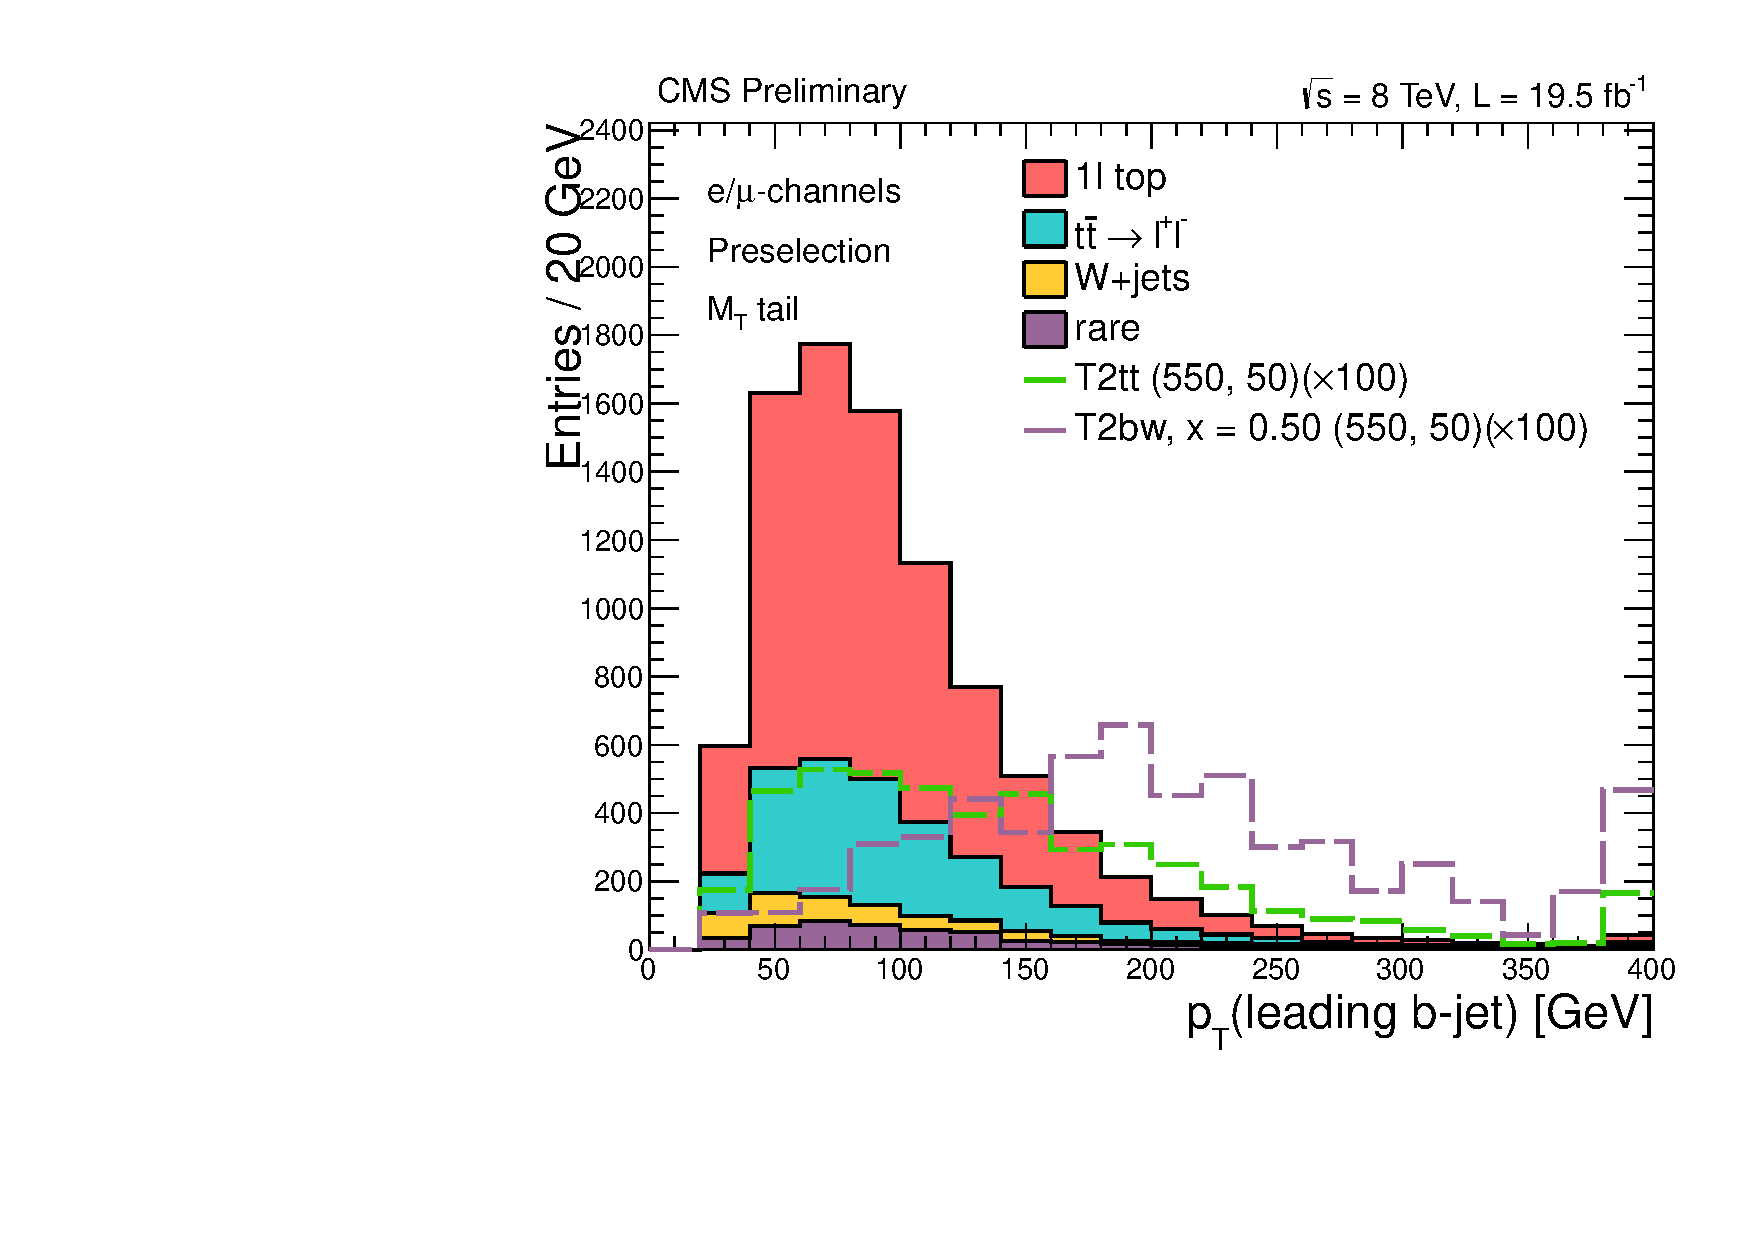
\includegraphics[width=0.32\textwidth]{variables/leadingBPt}
                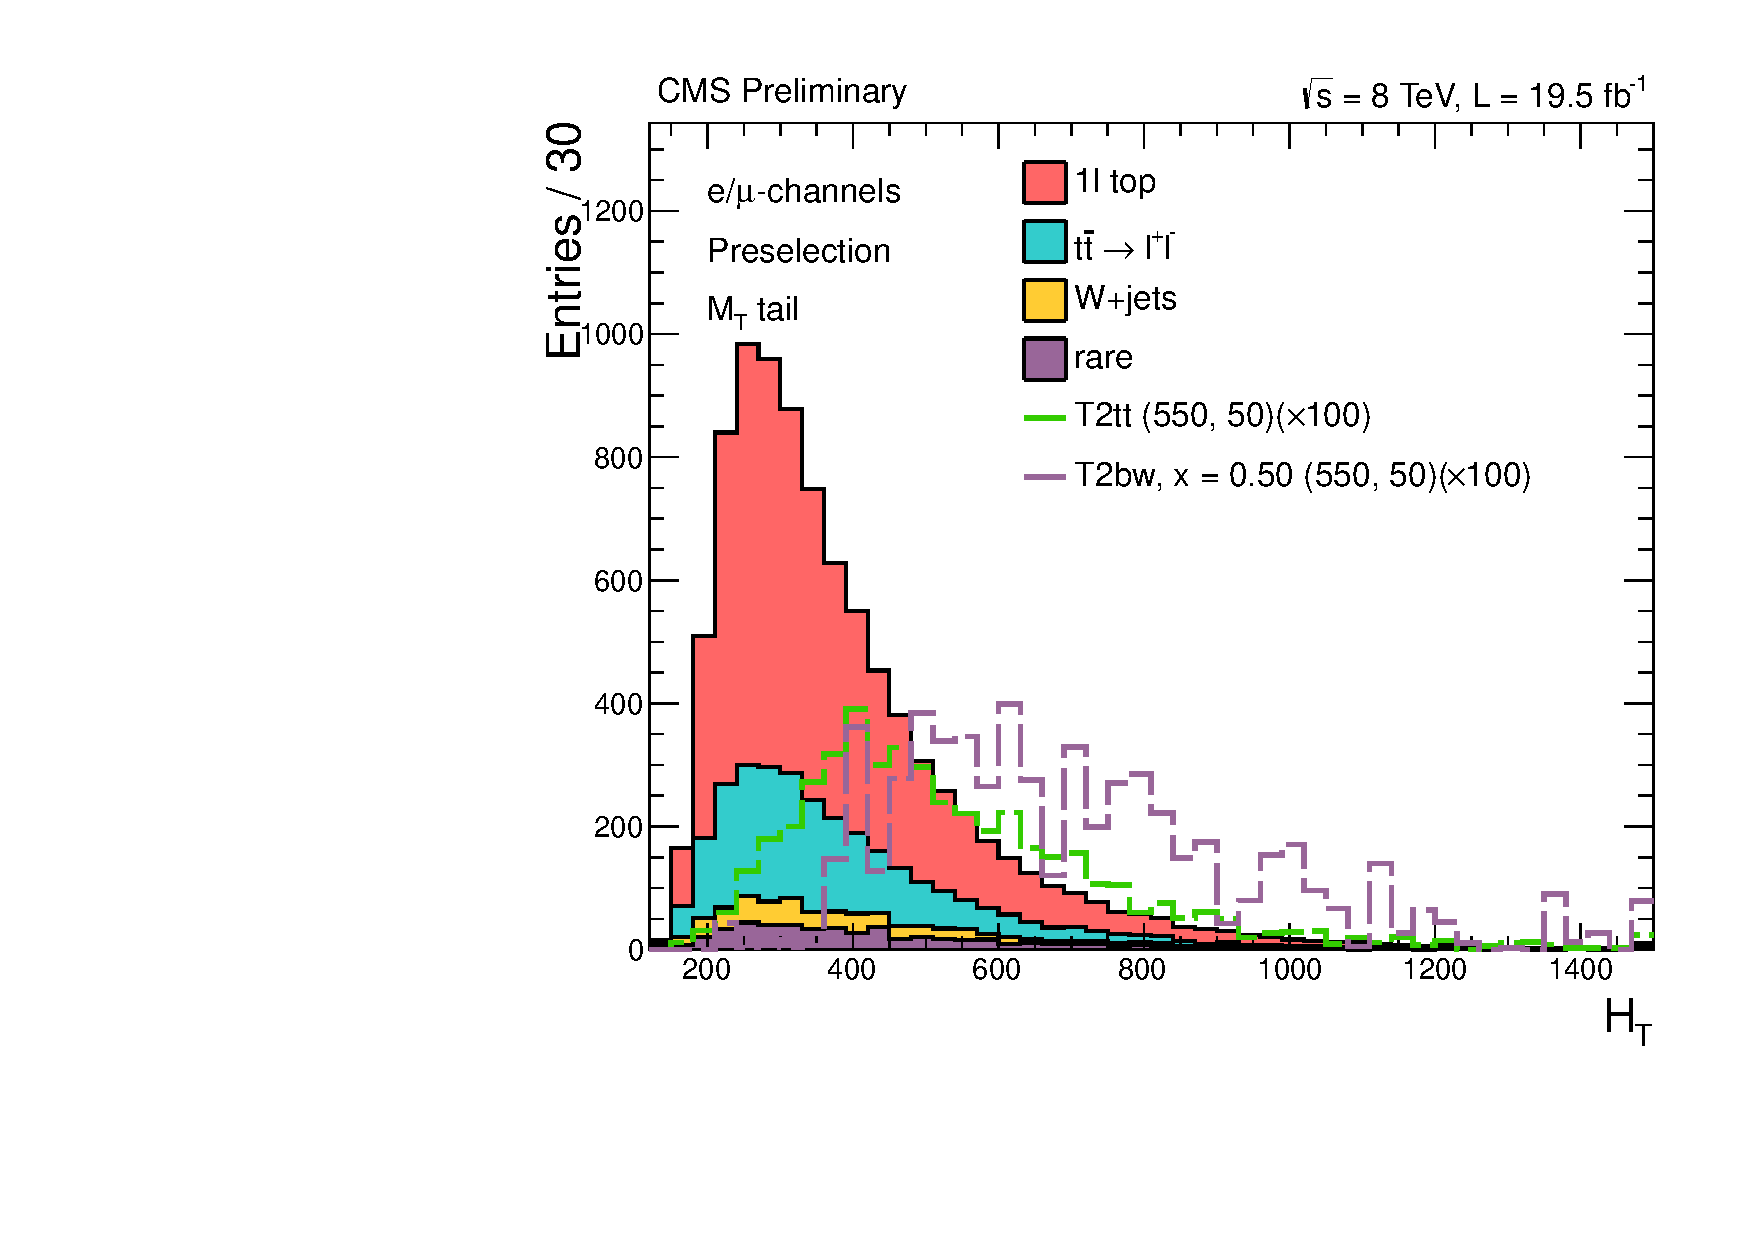
\includegraphics[width=0.32\textwidth]{variables/HT}
                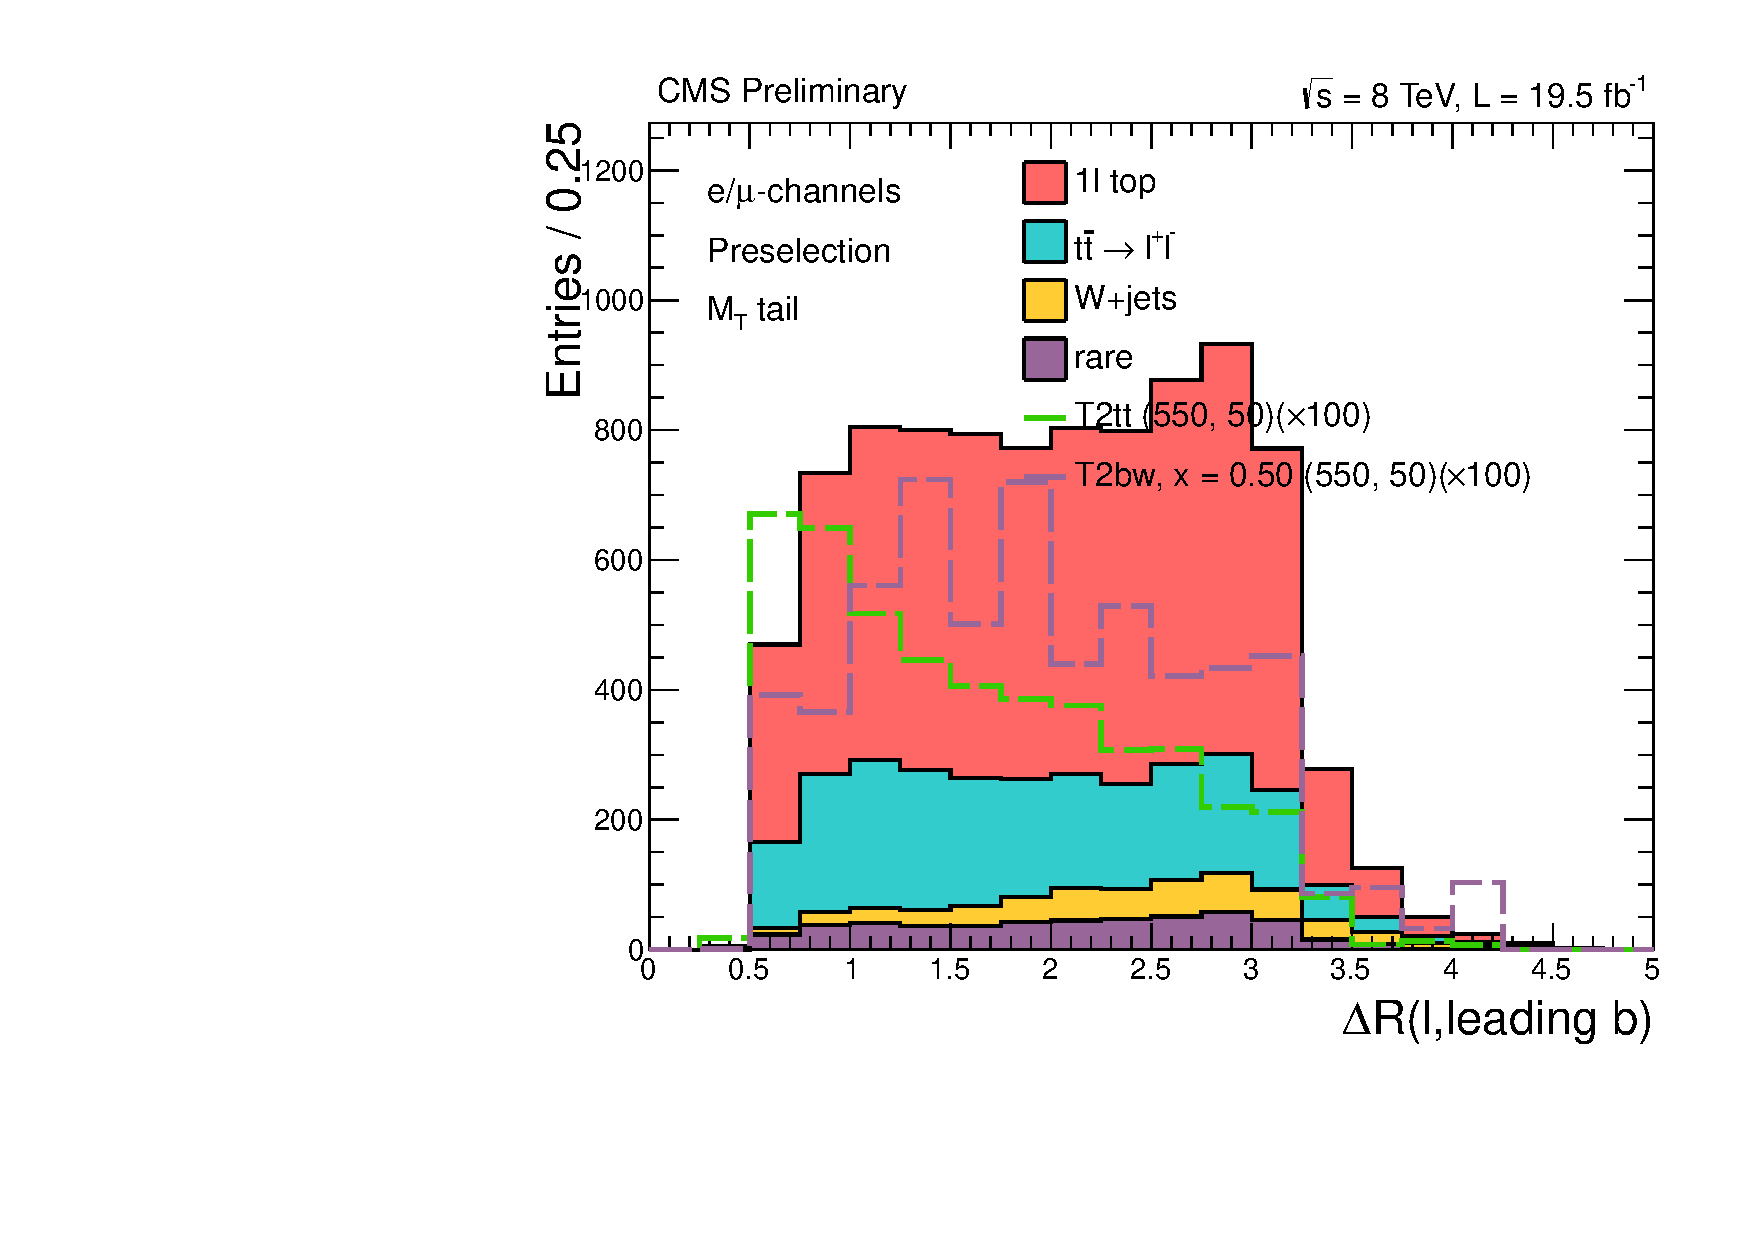
\includegraphics[width=0.32\textwidth]{variables/deltaRLeptonB}\\
                \includegraphics[width=0.32\textwidth]{variables/MET}
                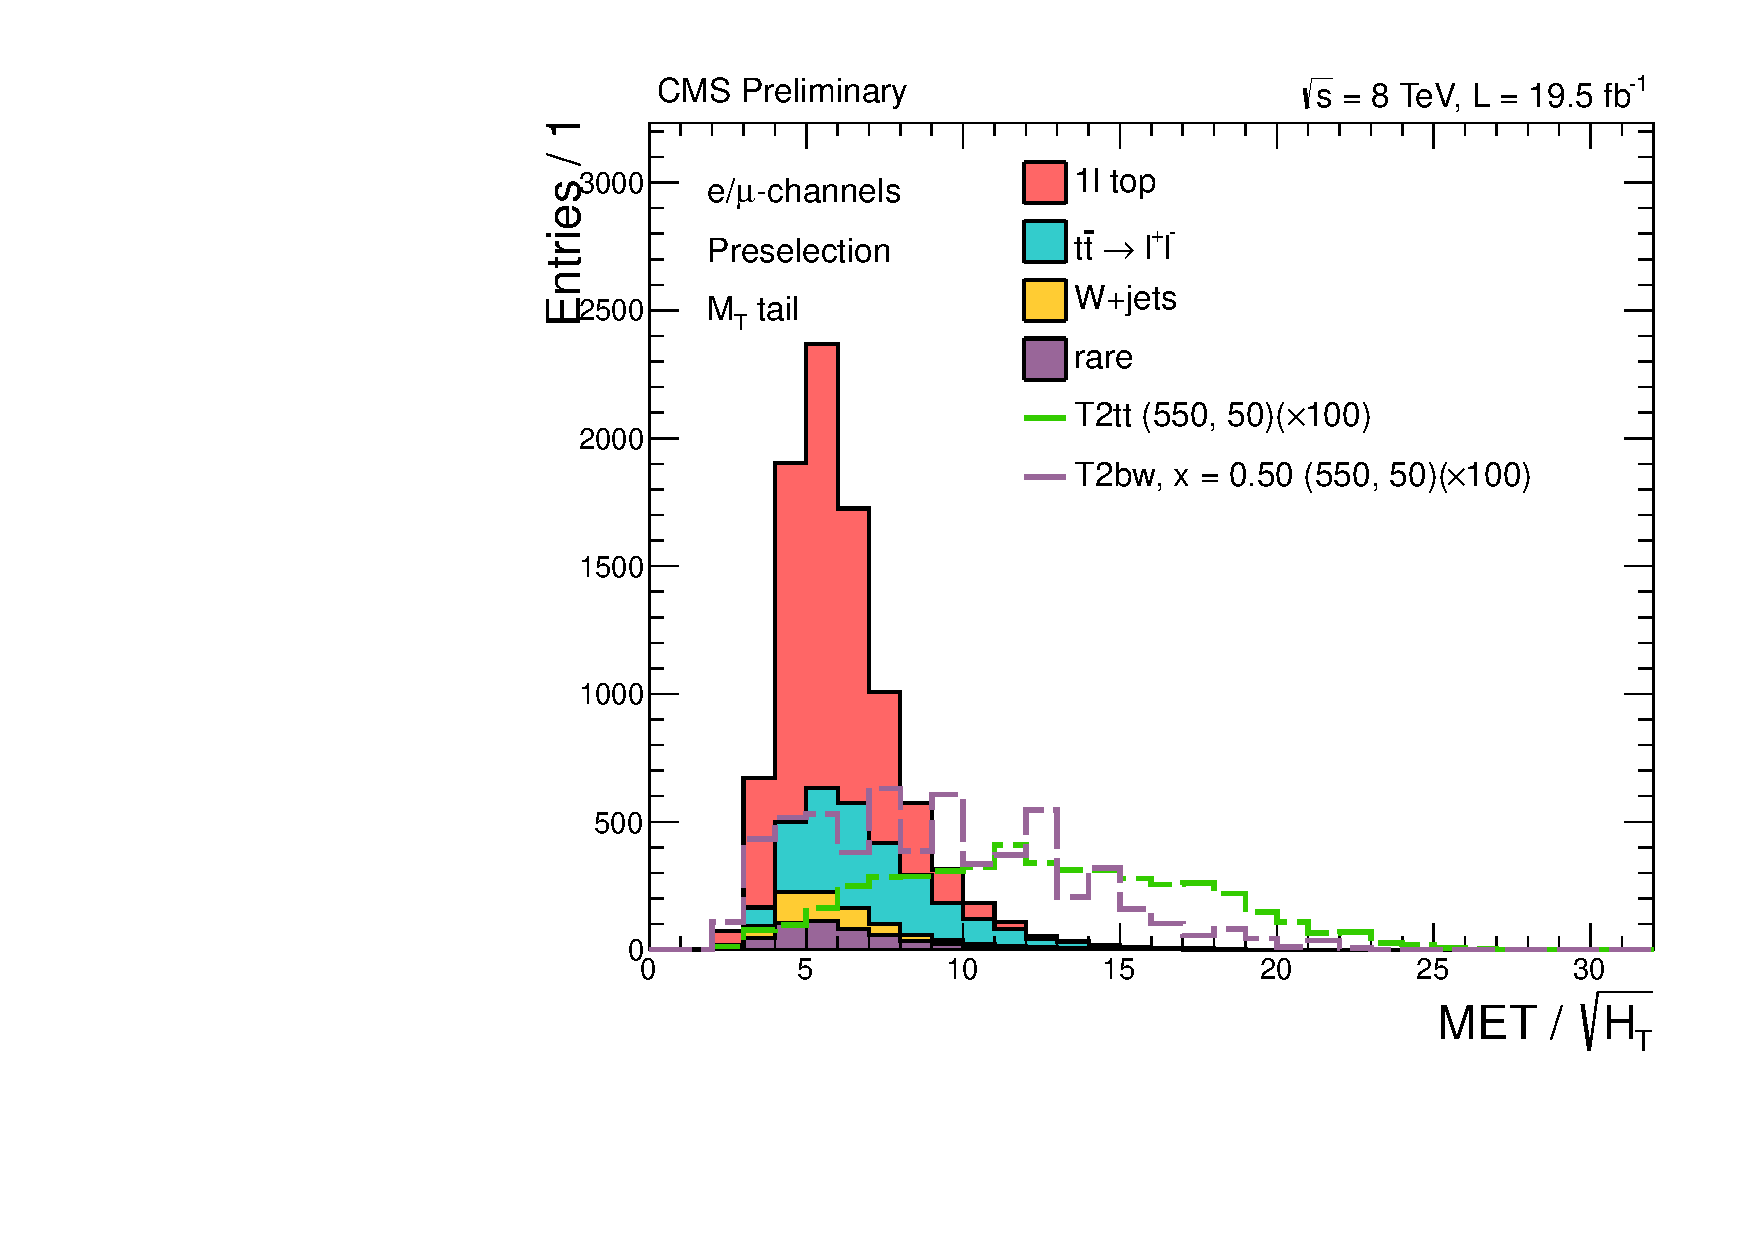
\includegraphics[width=0.32\textwidth]{variables/METoverSqrtHT}
                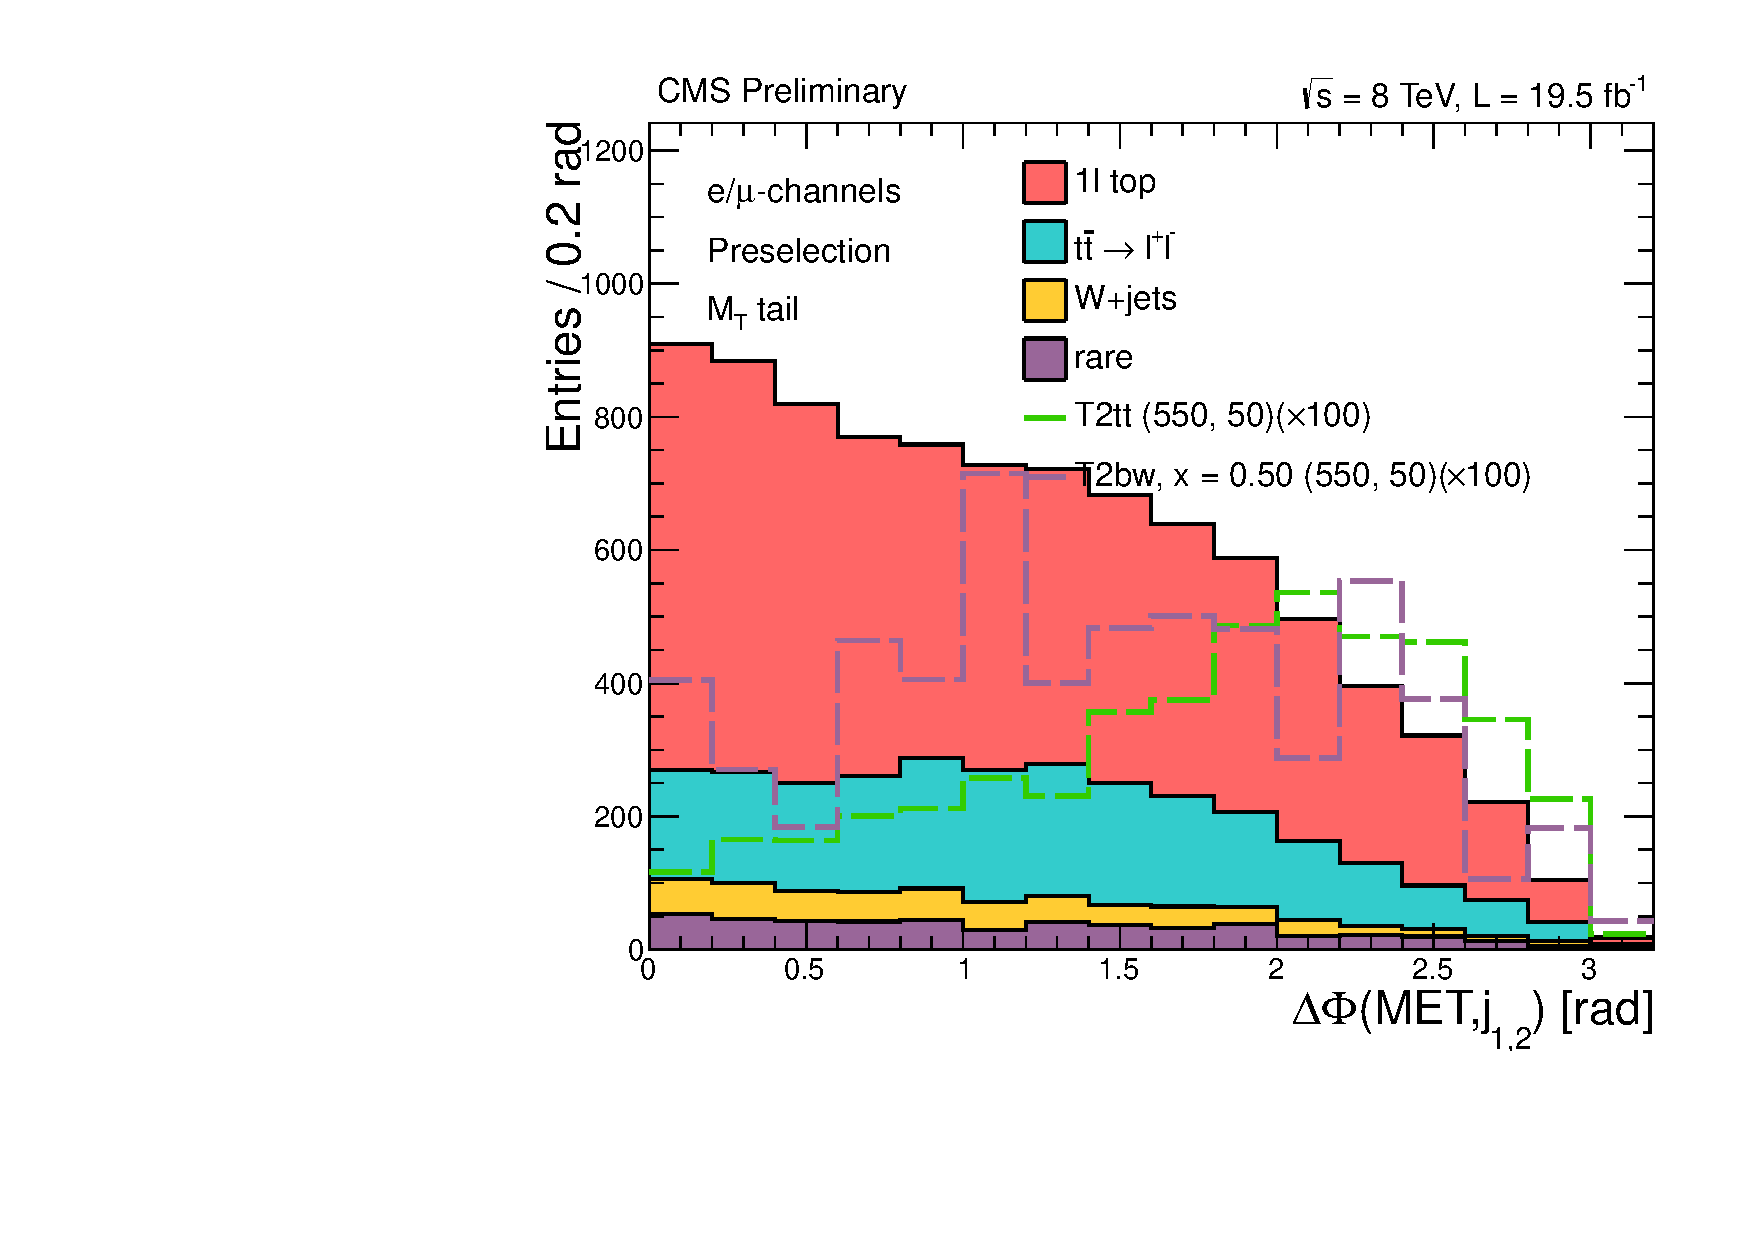
\includegraphics[width=0.32\textwidth]{variables/deltaPhiMETJets}\\
                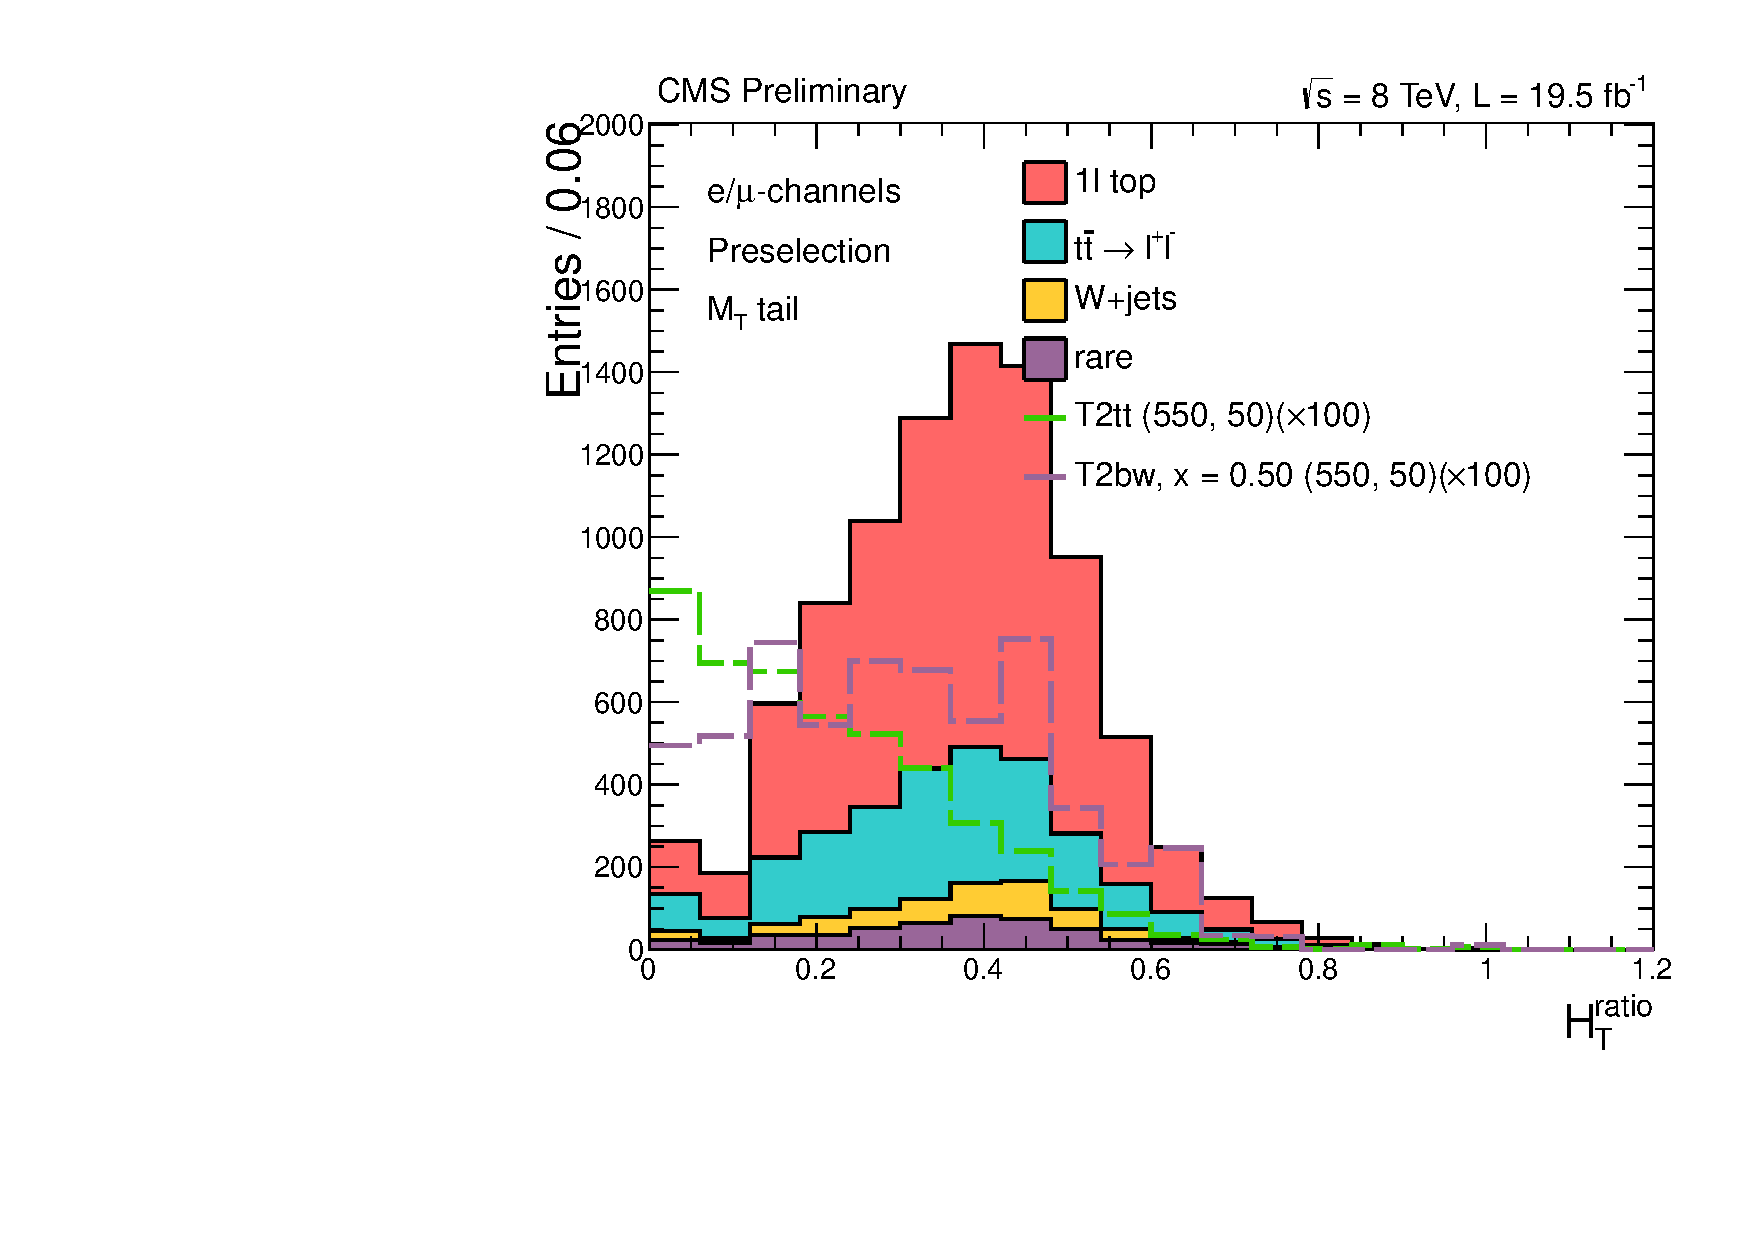
\includegraphics[width=0.32\textwidth]{variables/HTratio}
                \includegraphics[width=0.32\textwidth]{variables/MT2W}
                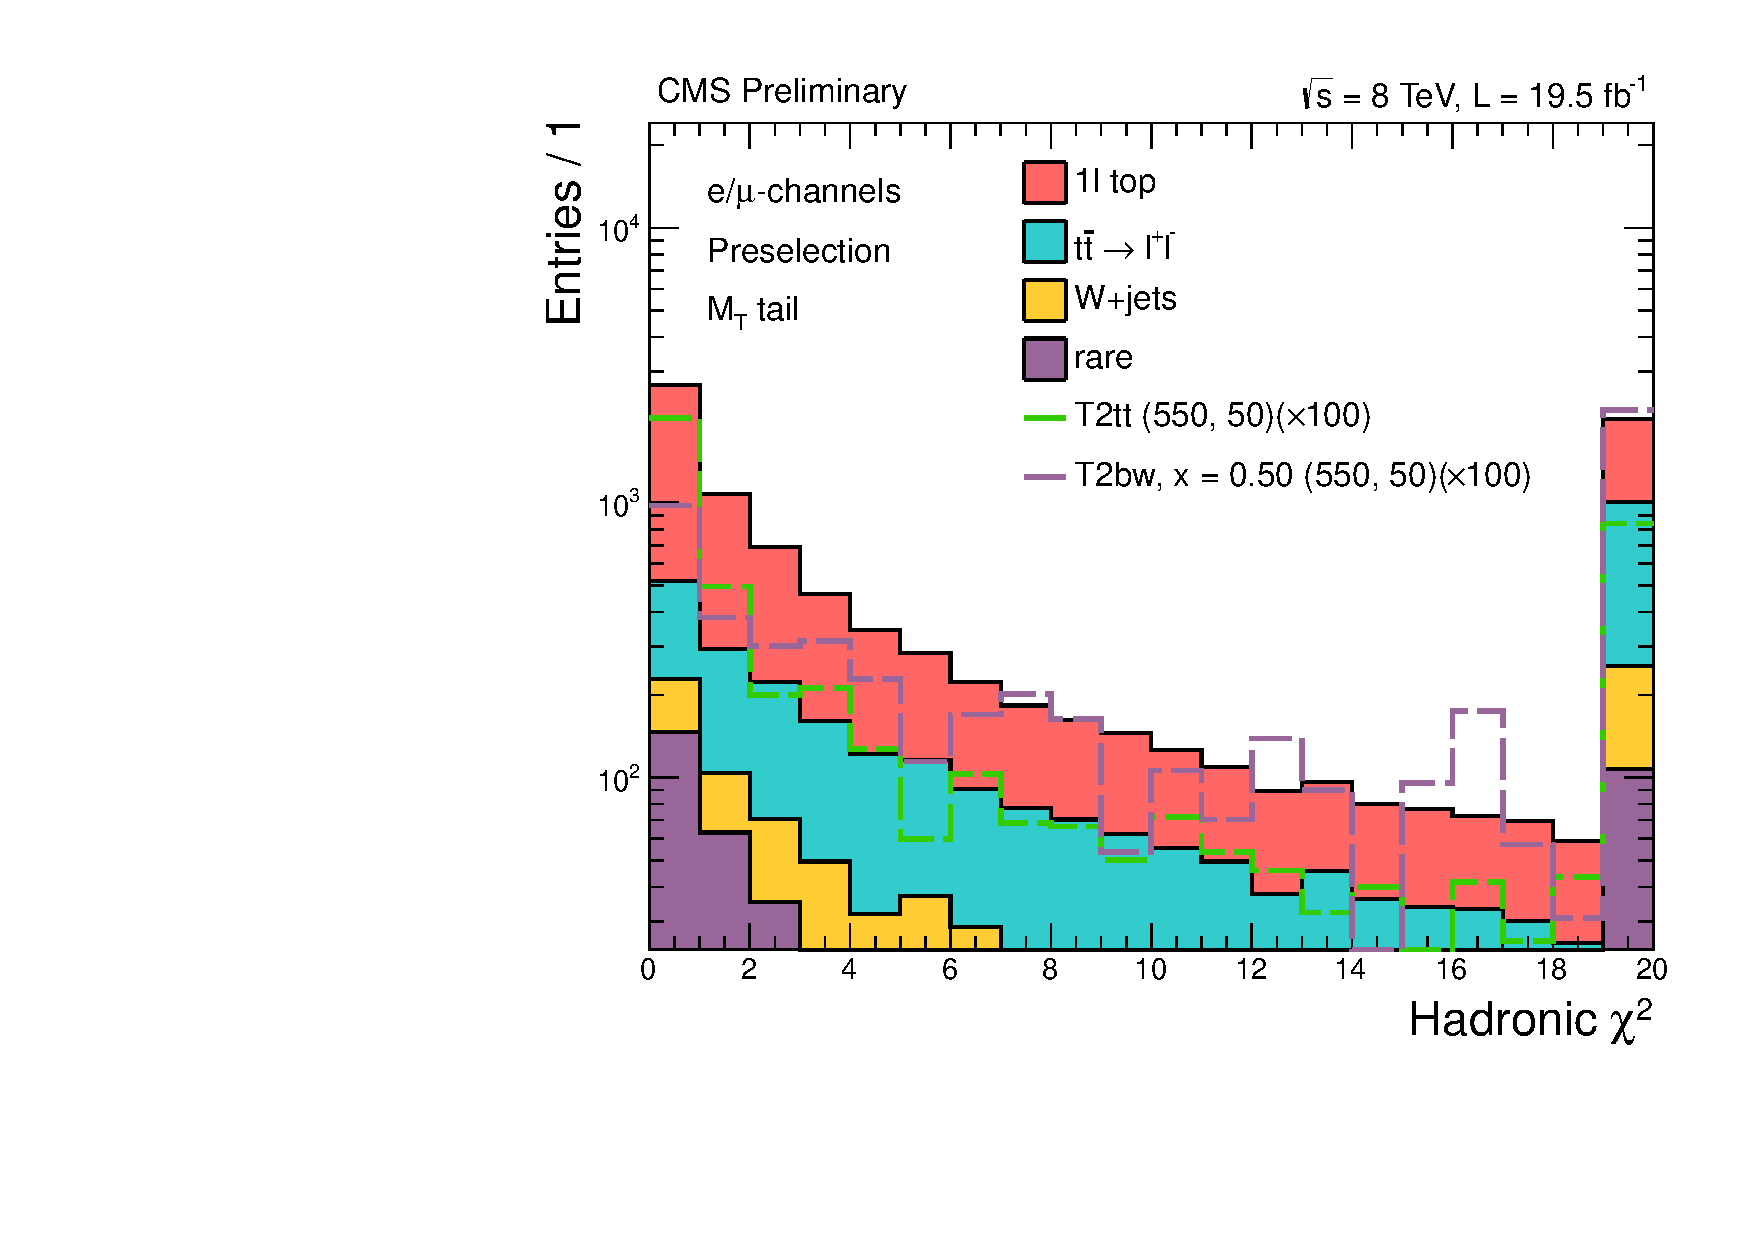
\includegraphics[width=0.32\textwidth]{variables/HadronicChi2}\\
                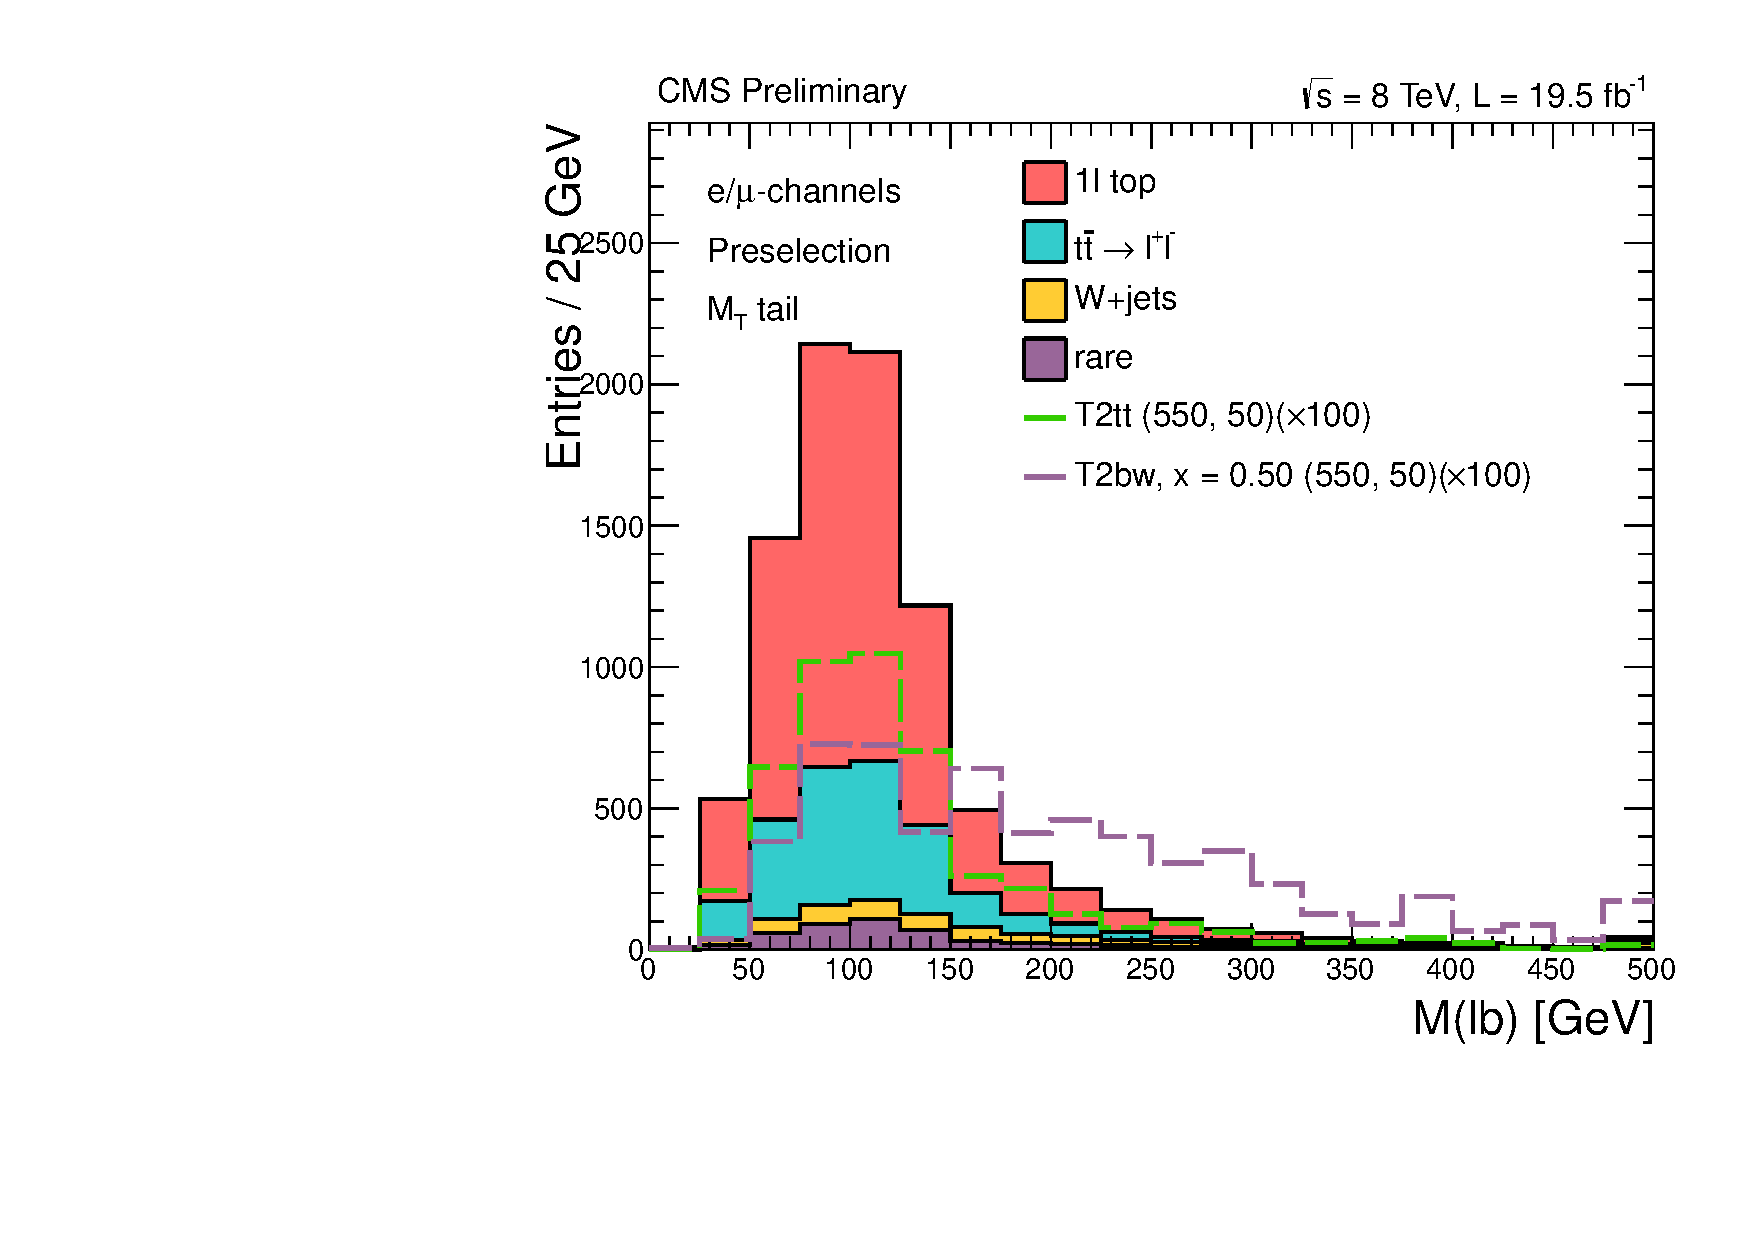
\includegraphics[width=0.32\textwidth]{variables/Mlb_hemi}
                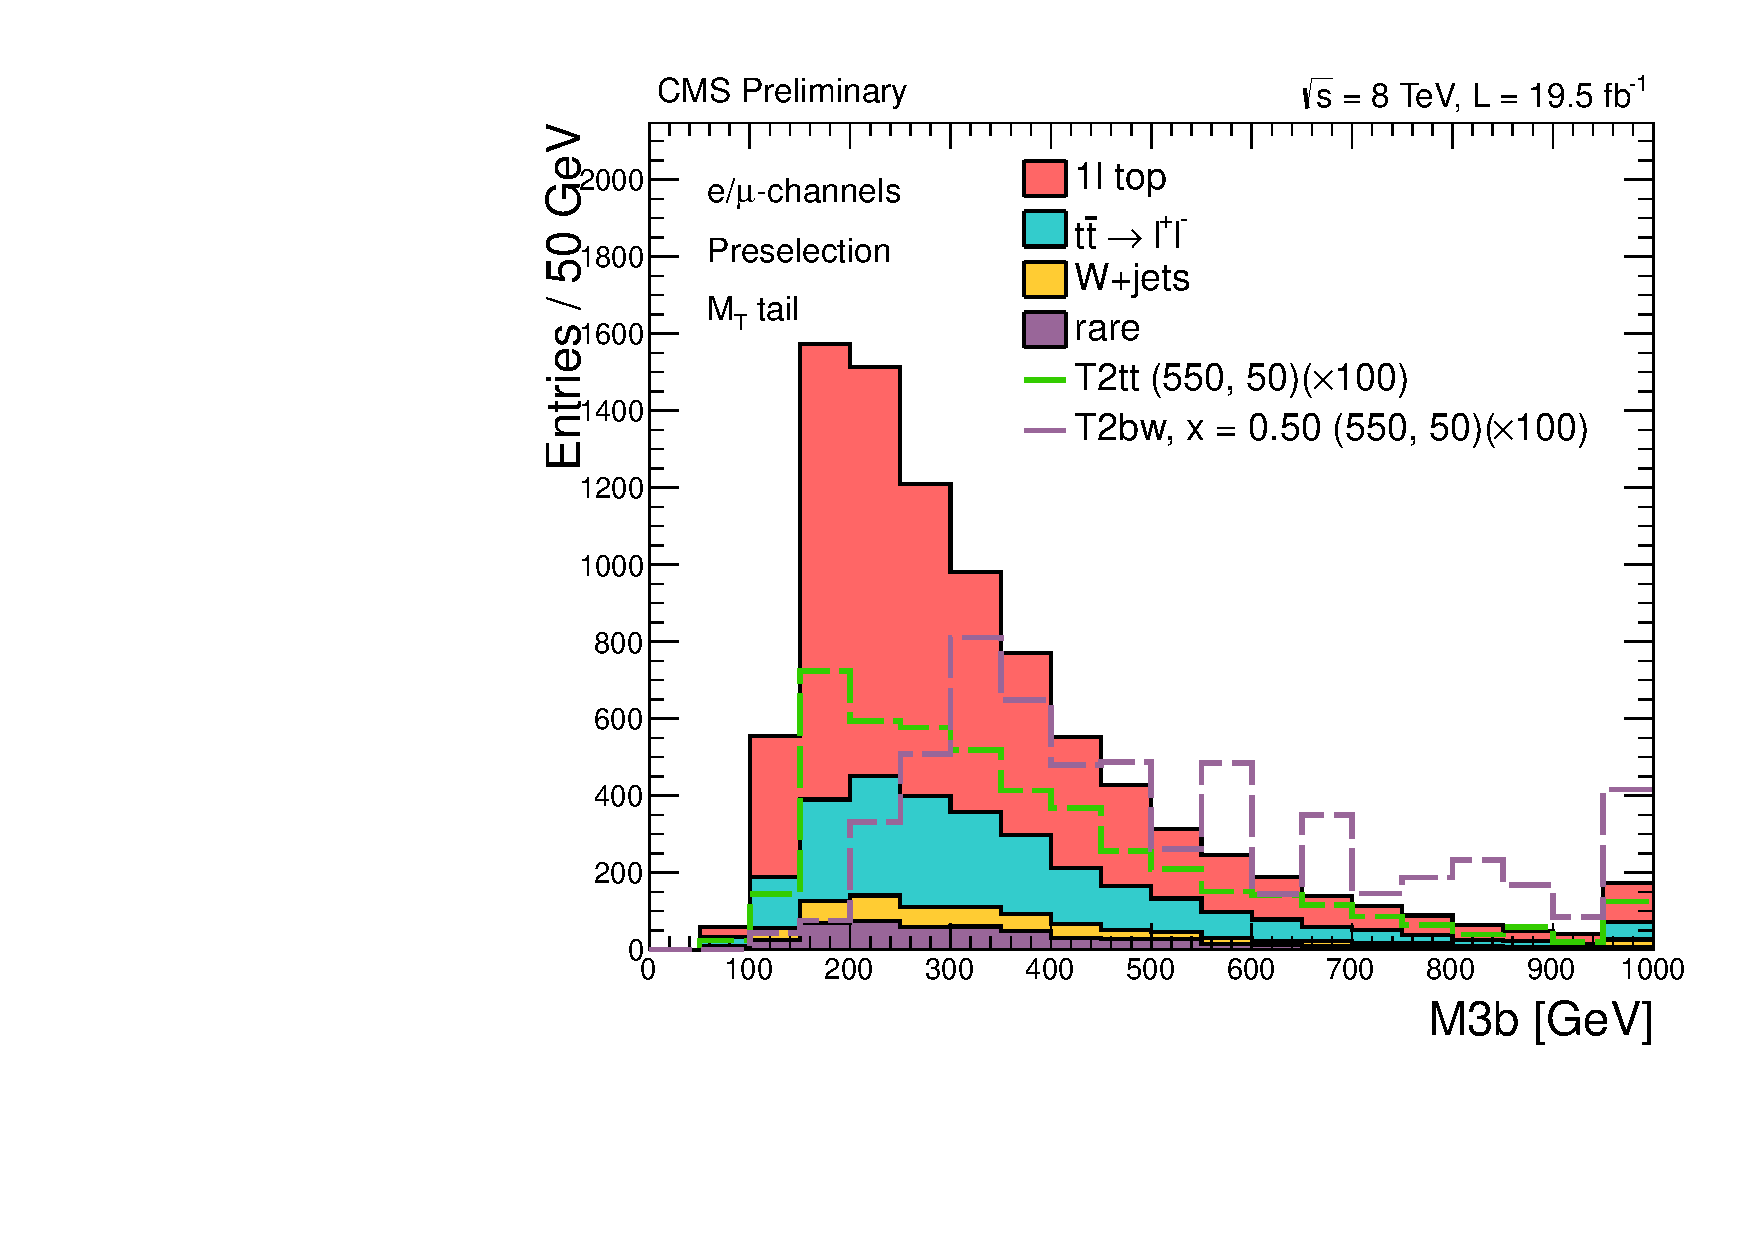
\includegraphics[width=0.32\textwidth]{variables/M3b}
                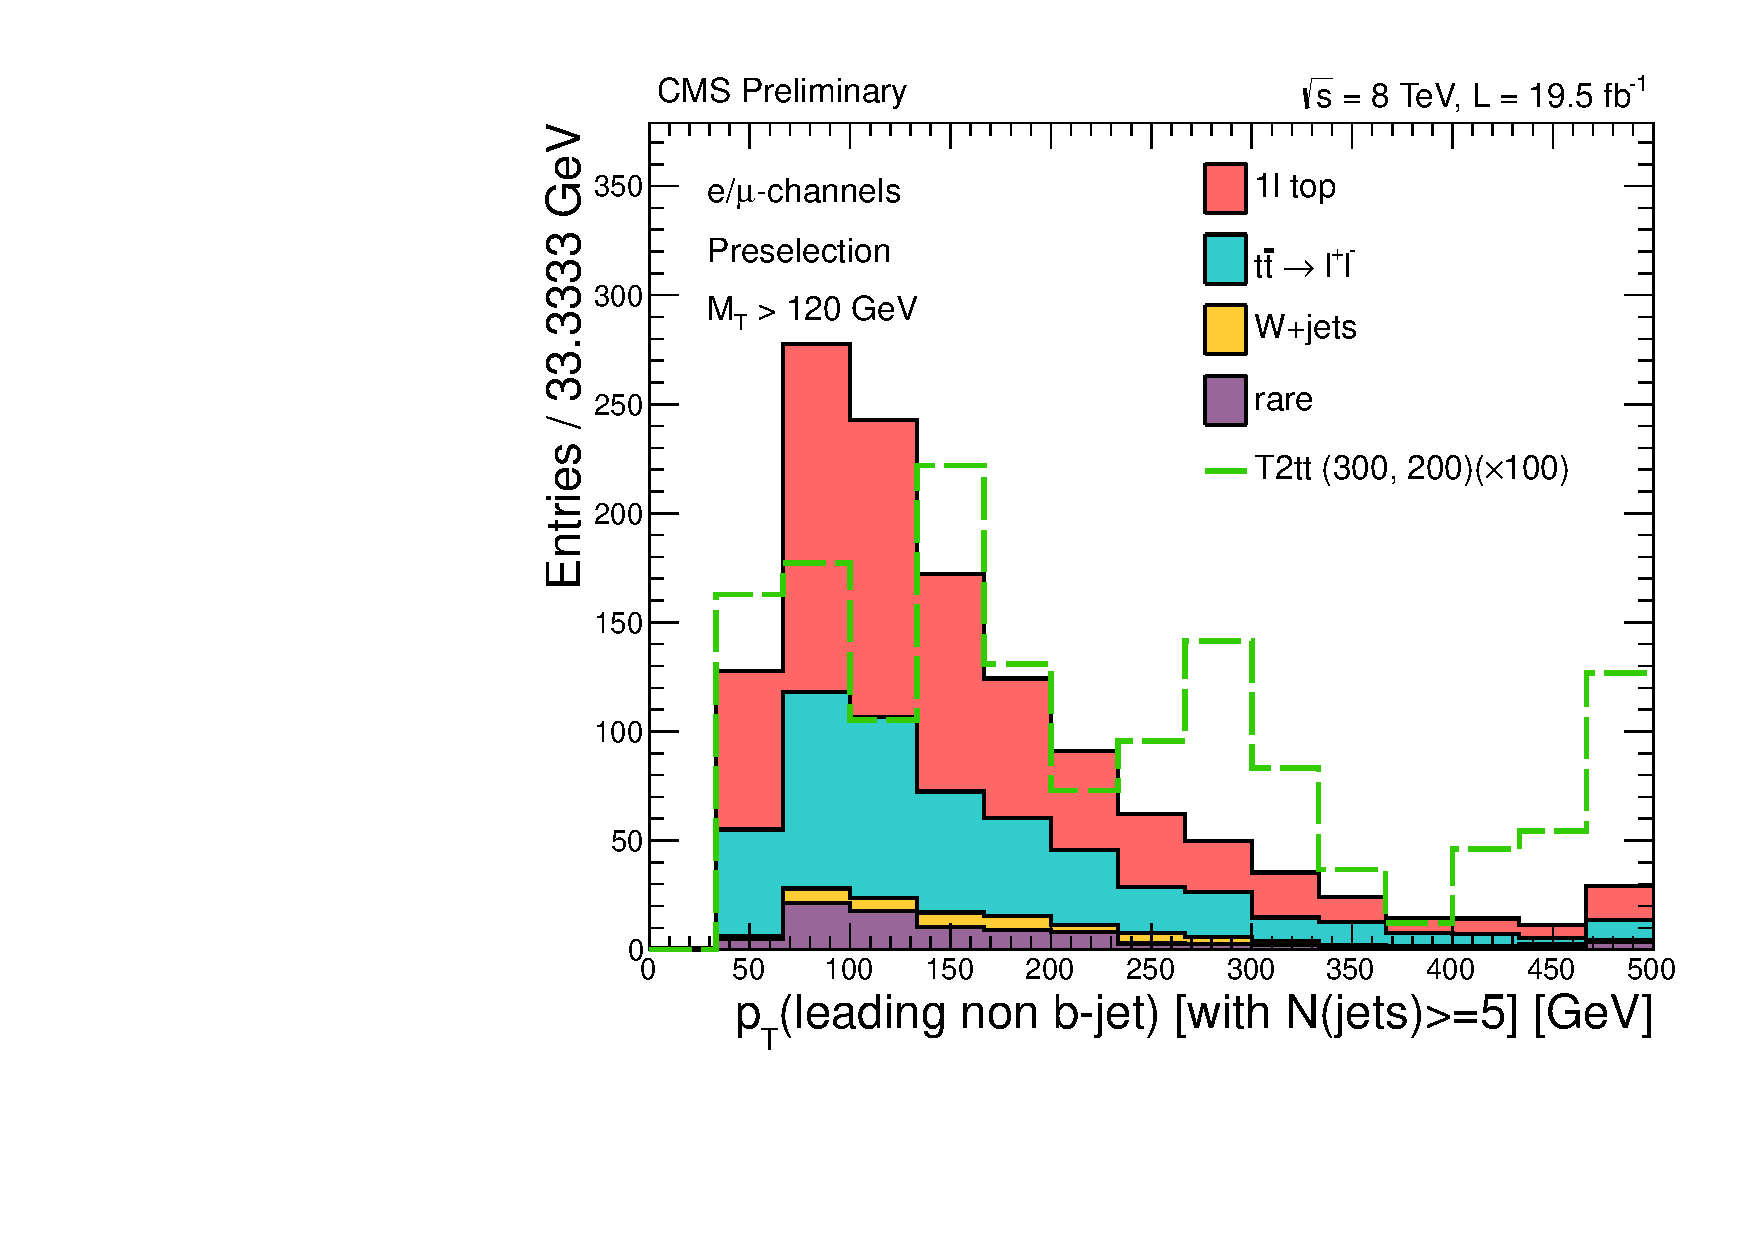
\includegraphics[width=0.32\textwidth]{variables/leadingNonBPtN5}
                \caption{Stacked plots representing the different discriminating variables used to design the signal region, for background and two signal examples after preselection and cut on $M_T > 100 \GeV$.
                \todo{update plot with missing variables and/or use same benchmark as previously, ie 450/50}}
                \label{fig:variables}
            \end{figure}

            \subsection{Figure of merit and sensitivity estimation}
            %==============================================================

    Before going into the details of the signal region optimization, we first need to
    introduce the metric used to do so. The problem of defining cuts to be applied on a
    variable can be summarized as knowing how to compromise between the quantity of
    selected signal, $S(\text{cut})$, versus selected background, $B(\text{cut})$, such
    that the sensitivity of the analysis is maximized. Ideally, one would run the full
    statistical interpretation which, in the context of the LHC experiments, is based
    on the $CL_S$ approach \refNeeded. However, such a procedure is CPU intensive as it is
    requires toy-data generation, and not suitable for a highly iterative process such
    as scanning possible cuts. In the case of a single-bin counting experiment, a more
    flexible way is to use analytical formula, called figure of merit (FoM) that gives an
    immediate estimation of the senstivity of the counting experiment.

    Let's consider the background only hypothesis $H_0$, also called null hypothesis,
    and the signal hypothesis $H_1$. These hypothesis are modeled by a probability density
    function (pdf), describing the probability to observe $N$ events in the data, as
    sketched on Figure \ref{fig:interpretation}.

    \insertFigure{interpretation}{0.7}
                 {Illustration of the modelization of the hypothesis $H_0$ and $H_1$ with
                 Poisson distributions of means and standard deviations being respectively
                 $(B,\sqrt{B})$ and $(S+B,\sqrt{S+B})$. \todo{fix plot}}

    From the point of view of excluding the signal hypothesis, a statistical hypothesis
    test consists in computing the probability $p$ to observe less than $D$ events in the
    data under $H_1$, $p(N < D|H_1)$. If this probability is lower than a treshold
    $\beta$, one may exclude the signal hypothesis with a confidence level $1-\beta$. A
    common practice is to use a confidence level of 95\%, or $\beta = 5\%$. The exclusion
    potential of a counting experiment can be defined via the probability $p(N < E[H_0]|H_1)$,
    i.e. the probability to observe a background-like realization in the data, if the
    signal exist. It is sometimes more pratical to express this potential in term of a
    significance $\mathcal{S}$, that is to say by expressing the distance $E[H_0] -
    E[H_1]$ in terms of standard deviations $\sigma[H_1]$ :

    $$ \mathcal{S}_\text{exclu.} = \frac{E[H_0] - E[H_1]}{\sigma[H_1]}$$

    If $H_1$ follows a gaussian distribution, then one can reinterpret $\mathcal{S}$ in terms
    of gaussian probabilities, for instance $\mathcal{S} = 2$ as a probability $p\approx5\%$
    using the so-called 68-95-99.7 rule of thumb in statistics. Considering that $H_0$ and
    $H_1$ have means and standard deviations being respectively $(B,\sqrt{B})$ and
    $(S+B,\sqrt{S+B})$ as in Figure \ref{fig:interpretation}, one ends up with

    $$ \mathcal{S}_\text{exclu.} = \frac{S}{\sqrt{S+B}}$$

    The same reasonning can be applied to the point of view of a discovery claim, where
    one is interested in $p(N > E[H_1]|H_0)$, i.e. the probability to observe a
    signal-like realization in the data, if the signal doesn't exist. Assuming the situation
    sketched in \ref{fig:interpretation}, one obtains a significance

    $$ \mathcal{S}_\text{disc.} = \frac{S}{\sqrt{B}}$$

    This significance definition can be easily used as a figure of merit when optimizing
    cuts. The picture may be completed by incoporating systematic uncertainties on the
    background to $\sigma[H_0]$ and $\sigma[H_1]$, leading to :

    \begin{equation}
       \mathcal{S}_\text{disc.} = \frac{S}{\sqrt{B+f^2 \cdot B^2}}
       \hspace*{2cm}
       \mathcal{S}_\text{exclu.} = \frac{S}{\sqrt{S+B+f^2 \cdot B^2}}
       \label{FoM}
   \end{equation}

    where $f$ represents an estimate of the relative systematic uncertainty on the background.

    While this figure of merit sometimes gives a reasonnable estimate of the true
    sensitivity of a counting experiment, one should remane conscious of its caveats
    \cite{Punzi} :

    \begin{enumerate}
        \item The intepretation of it is not straightfoward as it does not tell the
              physicist what can be expected to be excluded or discovered
              for a given counting experiment. It remains a 'number of sigmas', not an
              expected excluded cross-section.
        \item The formula \ref{FoM} does not contain any constrain regarding the fact that
              the observed number of events will be an integer. It will favorize a situation
              with $0.1$ signal events and expected background of $10^{-5}$ over a
              situation with 10 signal events and 1 background event, despite the fact that
              the later will definetely bring more information.
        \item It ultimately relies on a gaussian approximation which can cause significant
              discrepancies with respect to an accurate computation of $p(N|H)$. For instance,
              The Poisson and Gaussian tail integrals are significantly different at low
              means. More specifically, $\mathcal{S}_\text{disc.}$ is known to overestimate
              the true significance while $\mathcal{S}_\text{exclu.}$ underestimates it.
              Figure \ref{fig:} shows a comparison of $S/\sqrt{B}$ versus an exact
              computation.
    \end{enumerate}

    Caveat \#1 can be adressed by reinterpreting $\mathcal{S}$ in terms of excludable
    (or discoverable) signal strength $\mu$ or cross-section $\sigma$. Replacing
    $S$ with $\epsilon \times \sigma \times \mathcal{L}$, and introducing the discovery
    and exclusion treshold $a$ and $b$ (typically set to 5 and 2) yields :

    \begin{equation}
        \mathcal{\sigma}_\text{disc.} = a \cdot \frac{\sqrt{B+f^2B^2}}{\epsilon \cdot \mathcal{L}}
       \hspace*{2cm}
       \mathcal{\sigma}_\text{exclu.} = \frac{b}{2} \times \frac{b + \sqrt{b^2 + 4 (B + f^2B^2)}}{\epsilon \cdot \mathcal{L}}
       \label{FoM2}
    \end{equation}

    where $\epsilon$ and $\mathcal{L}$ are the selection efficiency and luminosity.

    Caveat \#2 can be worked around by imposing a minimum number of background and signal
    events when computing the figure of merit, for replacing $B$ with $\text{max}(B,1)$
    and ignoring cases with a too low expected signal yields.

    Finally, to address \#3, Ref. \cite{Punzi}, proposes an empirical fit to adjust the
    shape of the FoM with the accurate computation, as function of the parameters
    of the FoM. Alternative significances based on other approaches of the problem also
    exist and are discussed and compared in \todo{arXiv:physics/0702156v4 and arXiv:physics/0312059}.
    Figure \ref{fig:FOMcomparison} shows one of them, sometimes reffered to as Asimov Z and based on a
    likelihood approach, compared to the exact computation.

    \insertFigure{FOMcomparison}
                 {0.5}
                 {(From \todo{arXiv:1007:1727}, comparison of $S/\sqrt{B}$,
                 Asimov Z significance (denoted $\sqrt{q_{0,A}}$) and the exact significance computation
                 as function of $B$ and for $S = 2$, $5$ and $10$.}

        \subsection{Cut-based signal regions}
        %==============================================================

            \subsubsection{Optimization procedure}
            %==============================================================

    To design the cut-based signal regions on the analysis, the variables are first
    classified by their individual discriminating power, estimated by taking the
    maximum FoM achievable on a few signal benchmarks when scanning the possible
    cuts. The most discriminating variables are found to be $\MT$, $\MET$,
    $\MET/\sqrt{H_T}$ and $M_{T2}^{W}$. The variables $\Delta \phi(j_{1,2},\vec{\MET})$,
    hadronic top $\chi^2$, $\pT(\text{lead. } b)$ and the 5th, ISR jet requirement are
    also found to be helpful in particular cases or after cutting on the more discriminant
    variables. However we found that variables such as $H_T^\text{ratio}$, $M_{3b}$ and
    $M_{\ell b}$ offer lower potential.

    On a few signal benchmarks, we then proceed to a $n$-dimensionnal optimization of the
    cuts on these variables. We however impose some constrain in the use of the variables.
    First, either $\MET$ or $\MET/\sqrt{H_T}$ should be used, but not both at the same time.
    We allow tighter cuts on $\MT$ compared to the starting point $> 120\GeV$, but not
    tighter than $> 140\GeV$ especially to keep enough statistics for the background
    estimation related aspects.

    The optimization of the cuts is done with respect to the exclusion-oriented figure of
    merit defined in formula \ref{FoM}. To work around cases with very low background or signal leading,
    i.e. caveat \#2, we use $\tilde{B} \definedAs \text{max}(B,1)$ and set the FoM to 0
    if $S < 3$. The relative systematic uncertainty on the background is set to vary between
    15 and 30\% depending of the tightness of the cuts. We also incorporate some feedback
    of the background estimation that will be described later, by rescaling the $\oneLeptonTop$
    and $\Wjets$ contributions with a factor 1.3. This has for effect to favorize the
    rejection of these backgrounds over the $\diLeptonTop$ and rare components.

    After optimizing on a limited bunch of benchmarks, we inject all the sets of cuts found
    and map across the whole $(\mass{\lstop},\mass{\lneutralino)}$ space which is the one
    most performing set for each benchmark. As at this stage the number of set of cuts is
    large, and for the sake of keeping things manageable, we aim to reduce this number by
    manually clustering similar sets while keeping sure to not significantly loose in
    terms of performances.

            \subsubsection{Results and performances}
            %==============================================================

    The resulting signal regions definitions are presented on Table \ref{tab:cutAndCountCuts}.
    As announced in section \ref{sec:analysis_variables}, $\MET/\sqrt{H_T}$ tends to be
    preferred at low $\deltam$ compared to $\MET$. In the off-shell and stealthy regime,
    the ISR jet requirement plays an important role to gain sensitivity, despite the
    fact that this leaves little room for other cuts given the already low preselection
    efficiency and the tightness of requiring a 5th jet at high $p_T$.
    In the medium and high $\deltam$ regime, cutting on $M_{T2}^W$ provides a good gain
    in sensitivity because the large $\MET$ of the signal is less likely to decomposable
    in such a way that it fits the constrains while style yielding a light $m_Y$ mass.
    At low and medium $\deltam$ regimes for the $\lstop \rightarrow t \lneutralino$, the
    hadronic top $\chi^2$ provides a good alternative or complementary approach to $M_{T2}$
    for rejecting the $\diLeptonTop$ background. For $\lstop \rightarrow b \lchargino$,
    at low and medium $x$, the $\pT$ of the leading $b$ is an important feature, related
    to the high $\lstop-\lchargino$ gap. Finally, in almost all signal regions,
    $\Delta\phi(j_{1,2},\vec{\MET})$ proves to be useful by providing a way to reject the
    $\oneLeptonTop$ component where $\vec{\MET}$ is expected to be close to a ($b$-)jet.

    Figure \ref{fig:cutAndCountPerformances} shows the best performing set accross the
    $(\mass{\lstop},\mass{\lneutralino})$ plane as well as the corresponding FoM. While
    these results are purely based on the FoM, the final choice of the signal region to
    be used for each benchmark later done by choosing the minimum expected cross-section
    upper limit from the $CL_s$ computation.

\begin{table}[!ht]
{\footnotesize
\begin{center}
\hspace*{-0.8cm}
    \begin{tabular}{|l|ccccccc|}
    \hline
    $\lstop \rightarrow t\lneutralino$ & $\MT$   & $\MET$    & $\MET/\sqrt{H_T}$  & $M_{T2}^W$ & Hadronic top $\chi^2$ & $\Delta\phi(j_{1,2},\vec{\MET})$      &   5th, ISR jet \\
    \hline
    1) off-shell (loose)       & $>$ 125 & -       &   $>$ 8            &     -     & -             &          - &    yes        \\
    2) off-shell (tight)       & $>$ 130 & $>$ 300 &   -                &     -     & -        	    &          - &    yes        \\
    3) low    $\mass{\lstop}$  & $>$ 140 & -       &   $>$ 8            &     -     &  $<$ 5        &  $>$ 0.8   &    -          \\
    4) medium $\deltam$        & $>$ 140 & $>$ 200 &   -                &  $>$ 180  &  $<$ 3        &  $>$ 0.8   &    -          \\
    5) high   $\deltam$        & $>$ 130 & $>$ 350 &   -                &  $>$ 190  & -             &          - &    -          \\
        \hline
    \end{tabular}
    \hspace*{-0.5cm}
    \begin{tabular}{|l|ccccccc|}
    \hline
    $\lstop \rightarrow b\lchargino, x=0.25$   & $\MT$     & $\MET$    & $\MET/\sqrt{H_T}$ & $M_{T2}^W$ & $\pT(\text{lead. }b)$ & $\Delta\phi(j_{1,2},\vec{\MET})$ & 5th, ISR jet  \\
    \hline
    1) off-shell        & $>$ 120   &  -       &    $>$  9       &     -      &   -                   &  $>$ 0.2      & yes           \\
    2) low    $\deltam$ & $>$ 120   &  -       &    $>$  6       &  $>$ 200   & $>$ 180               &  $>$ 0.8      & -             \\
    3) high   $\deltam$ & $>$ 120   & $>$ 300  &     -           &  $>$ 200   & $>$ 180               &  $>$ 0.8      & -             \\
    \hline
    $\lstop \rightarrow b\lchargino, x=0.50$     & $\MT$     & $\MET$    & $\MET/\sqrt{H_T}$ & $M_{T2}^W$ & $\pT(\text{lead. }b)$ & $\Delta\phi(j_{1,2},\vec{\MET})$ & 5th, ISR jet  \\
    \hline
    1) off-shell        &  $>$ 120  &   -      &  $>$  9         &    -       & -                     &  $>$ 0.2      & yes           \\
    2) low masses       &  $>$ 135  &   -      &  $>$  6         & $>$ 180    & -                     &  $>$ 0.8      & -             \\
    3) medium $\deltam$ &  $>$ 140  &   -      &  $>$  7         & $>$ 190    & $>$ 100               &  $>$ 0.8      & -             \\
    4) high   $\deltam$ &  $>$ 120  & $>$ 300  &   -             & $>$ 200    & $>$ 100               &  $>$ 0.8      & -             \\
    \hline
    $\lstop \rightarrow b\lchargino, x=0.75$   & $\MT$     & $\MET$    & $\MET/\sqrt{H_T}$ & $M_{T2}^W$ & $\pT(\text{lead. }b)$ & $\Delta\phi(j_{1,2},\vec{\MET})$ & 5th, ISR jet  \\
    \hline
    1) low    $\deltam$ &  $>$ 120  &   -      &  $>$  12        &     -      &      -                &  $>$ 0.8      & yes           \\
    2) medium $\deltam$ &  $>$ 130  &   -      &  $>$  10        &  $>$ 180   &      -                &  $>$ 0.8      & -             \\
    3) high   $\deltam$ &  $>$ 140  & $>$ 300  &    -            &  $>$ 200   &      -                &  $>$ 0.8      & -             \\
    \hline
    \end{tabular}
\caption{Description of the signal regions defined and optimized for the cut-based approach. \label{tab:cutAndCountCuts}}
\end{center}}
\end{table}


            \begin{figure}[h!]
                \centering
                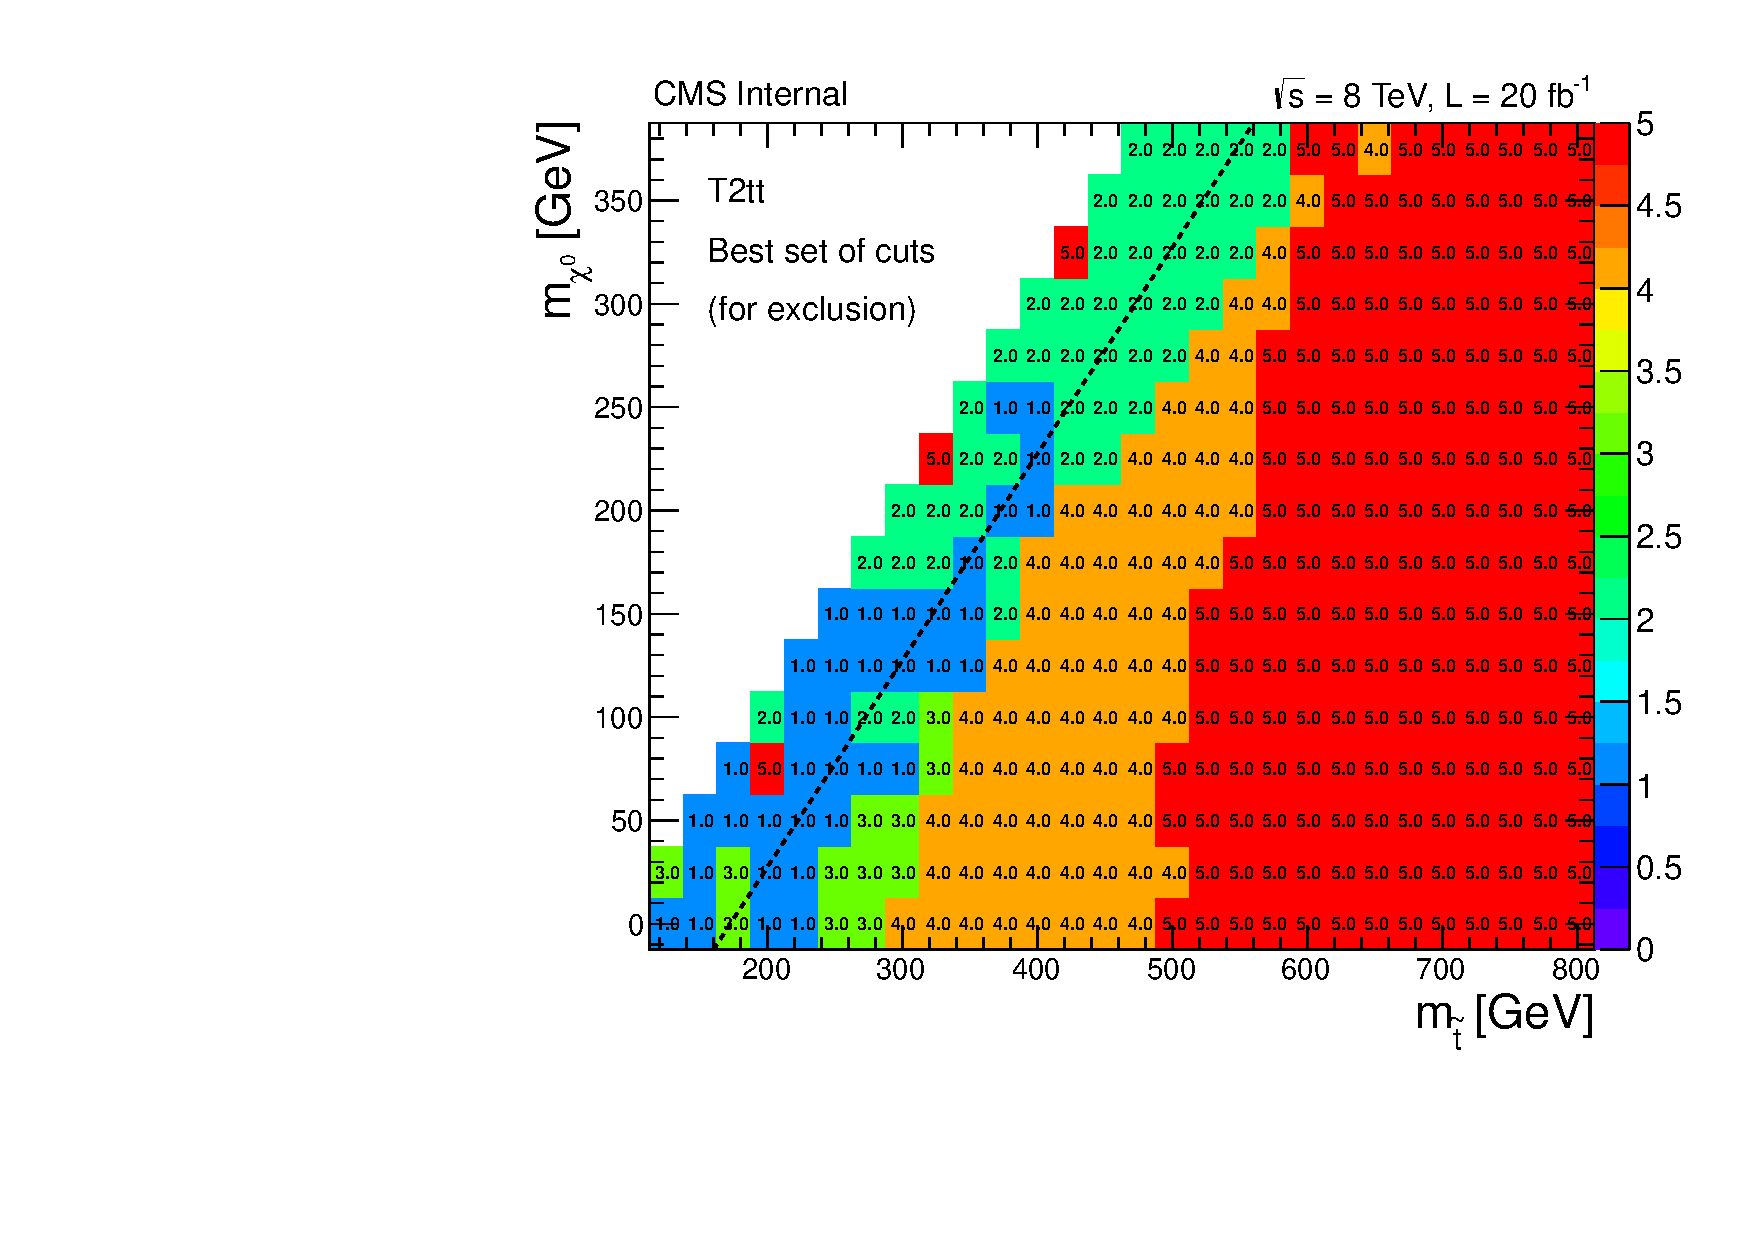
\includegraphics[width=0.37\textwidth]{cutAndCountPerformances/bestSet_T2tt}
                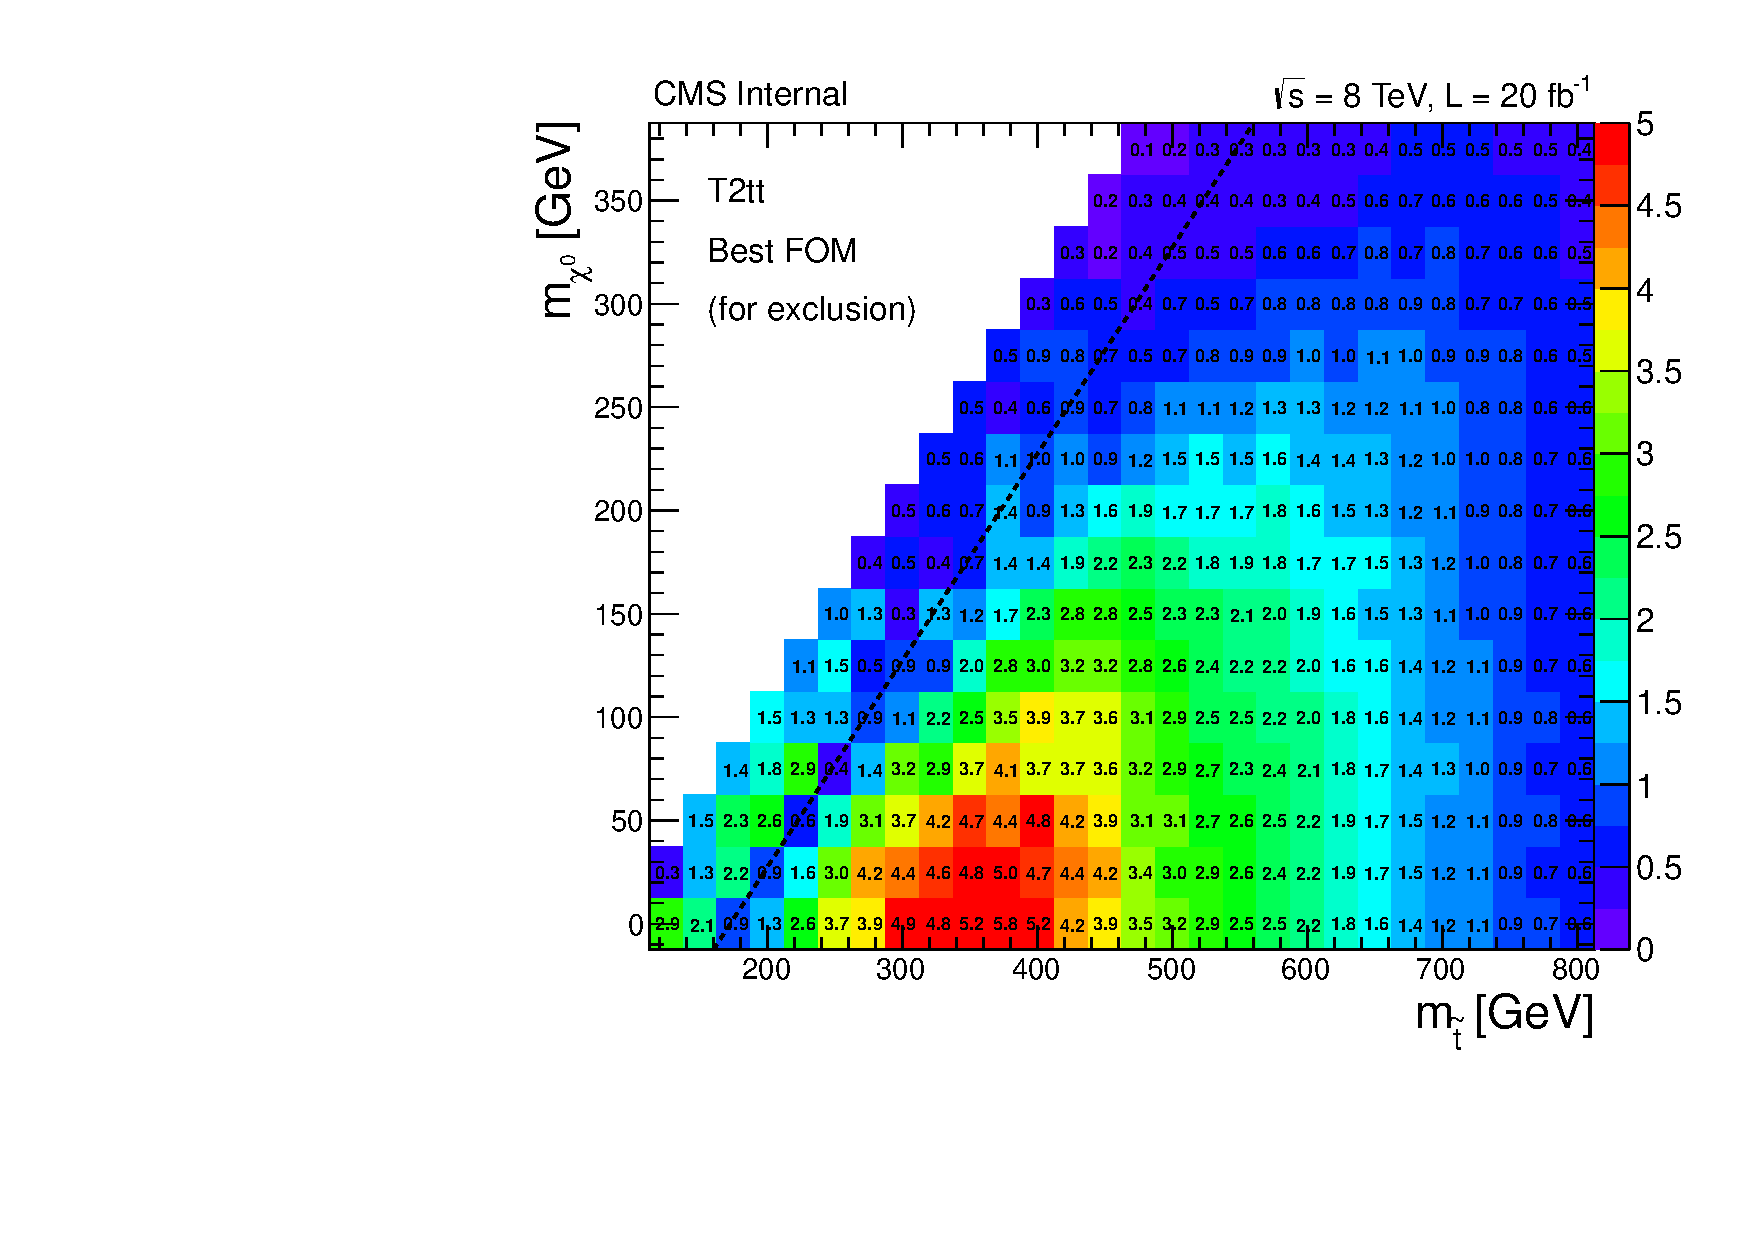
\includegraphics[width=0.37\textwidth]{cutAndCountPerformances/bestFOM_T2tt}\\
                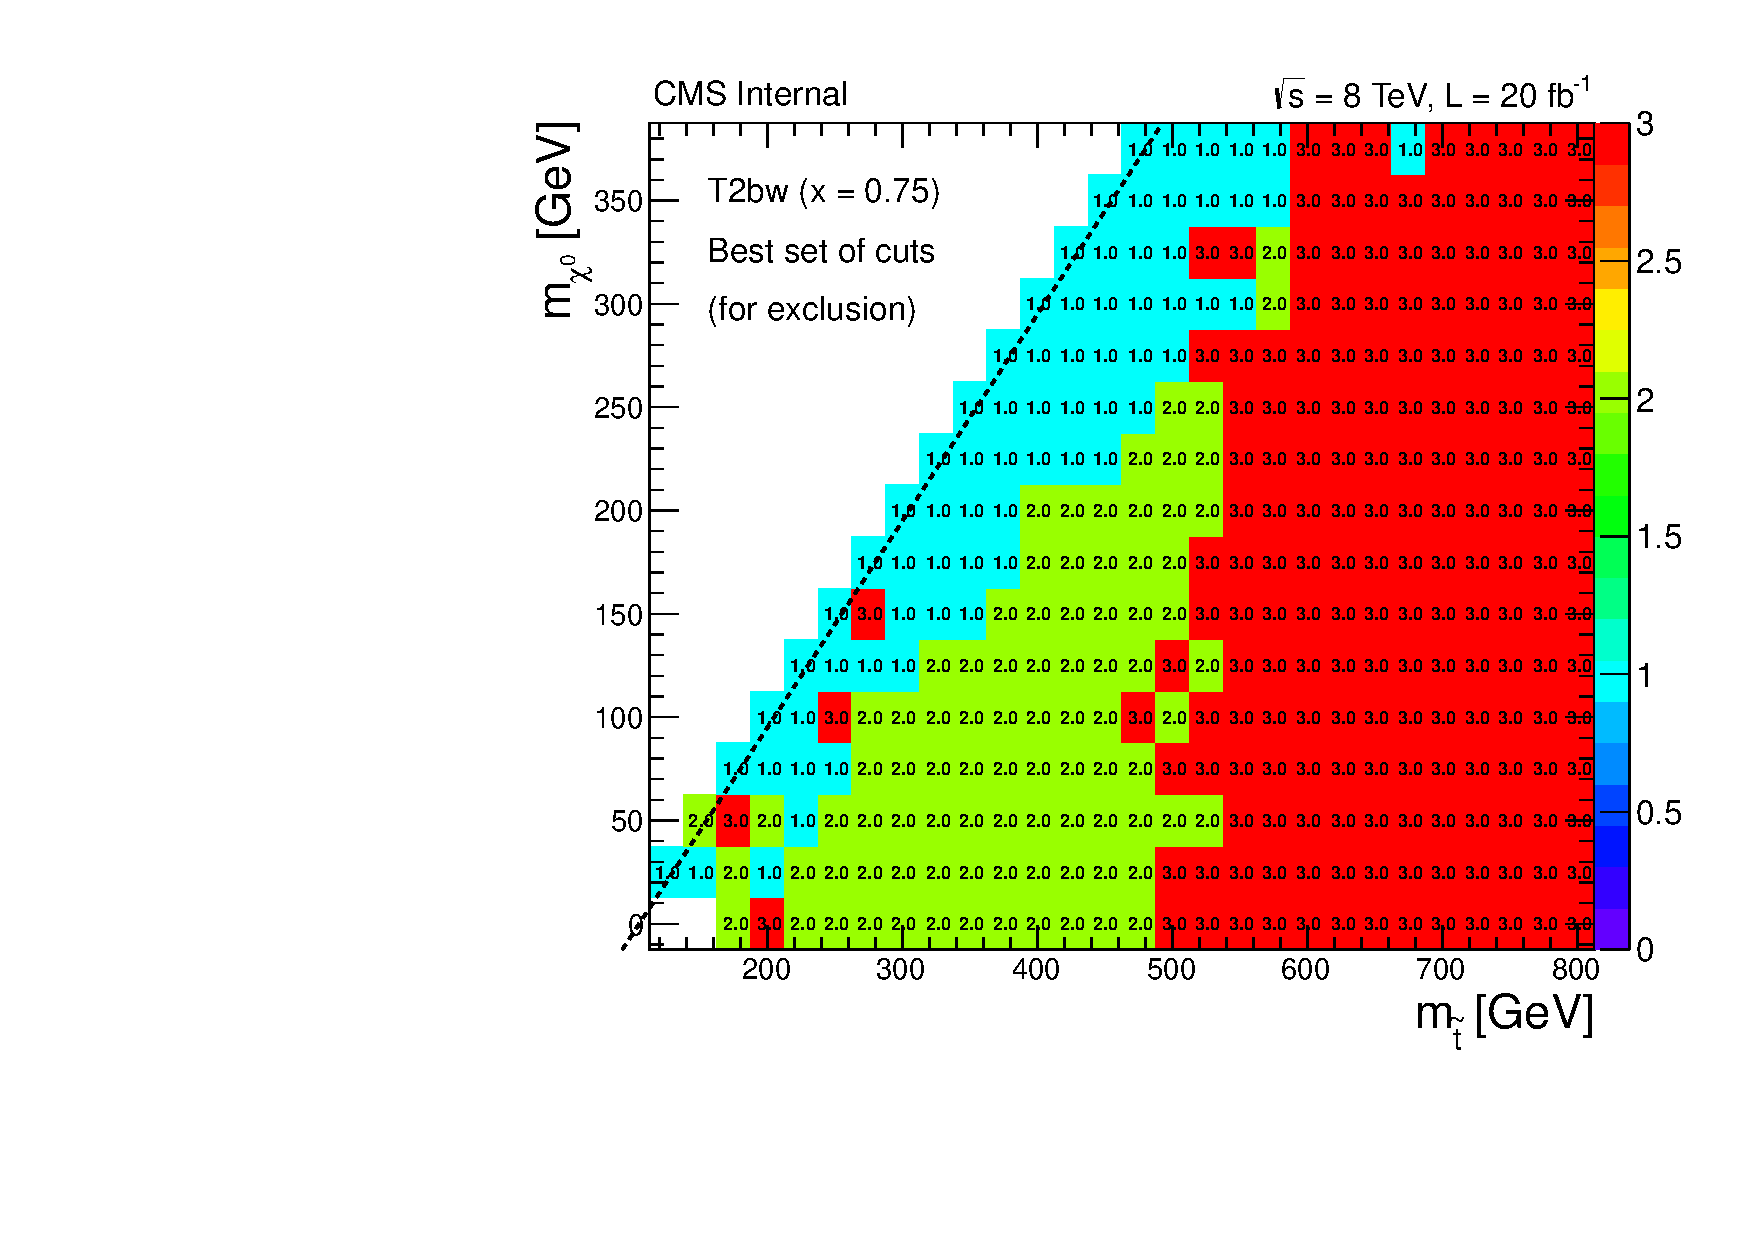
\includegraphics[width=0.37\textwidth]{cutAndCountPerformances/bestSet_T2bw075}
                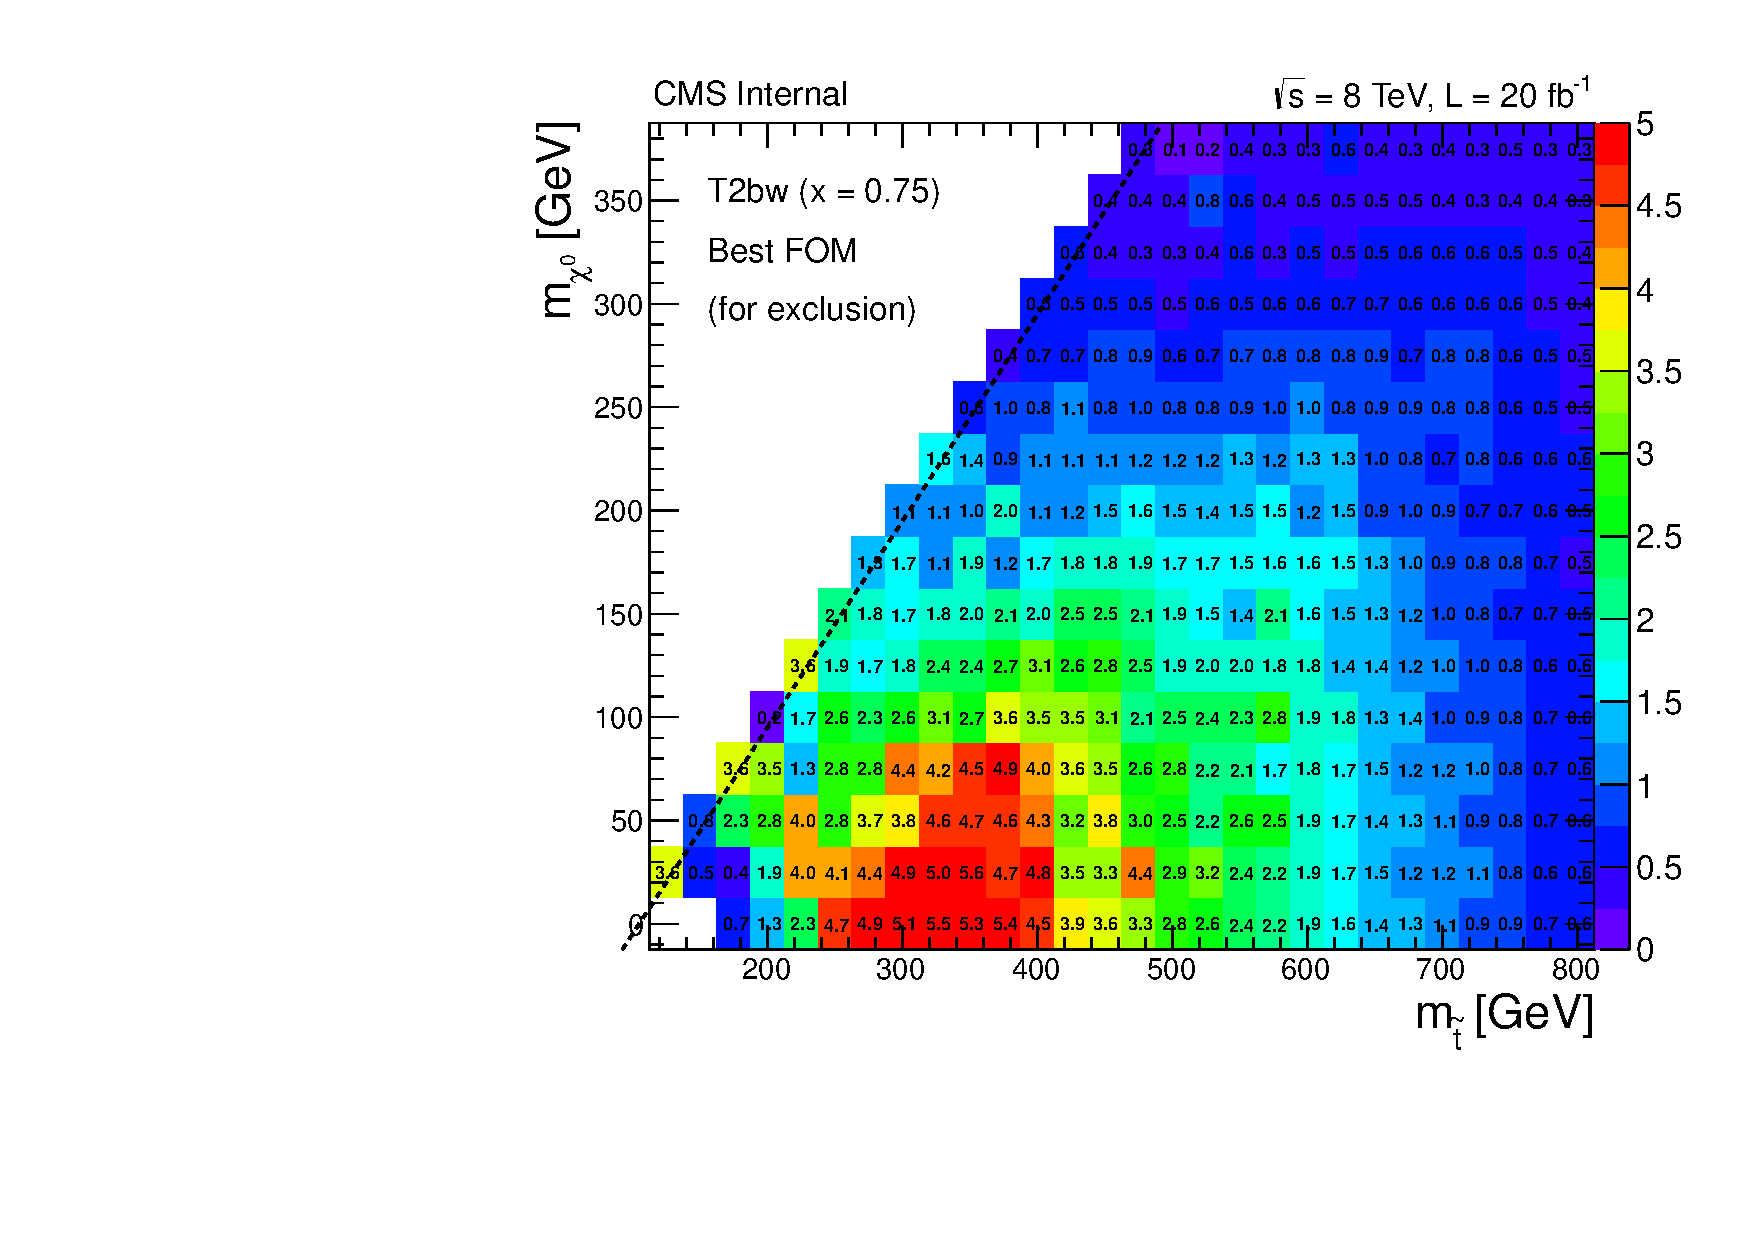
\includegraphics[width=0.37\textwidth]{cutAndCountPerformances/bestFOM_T2bw075}\\
                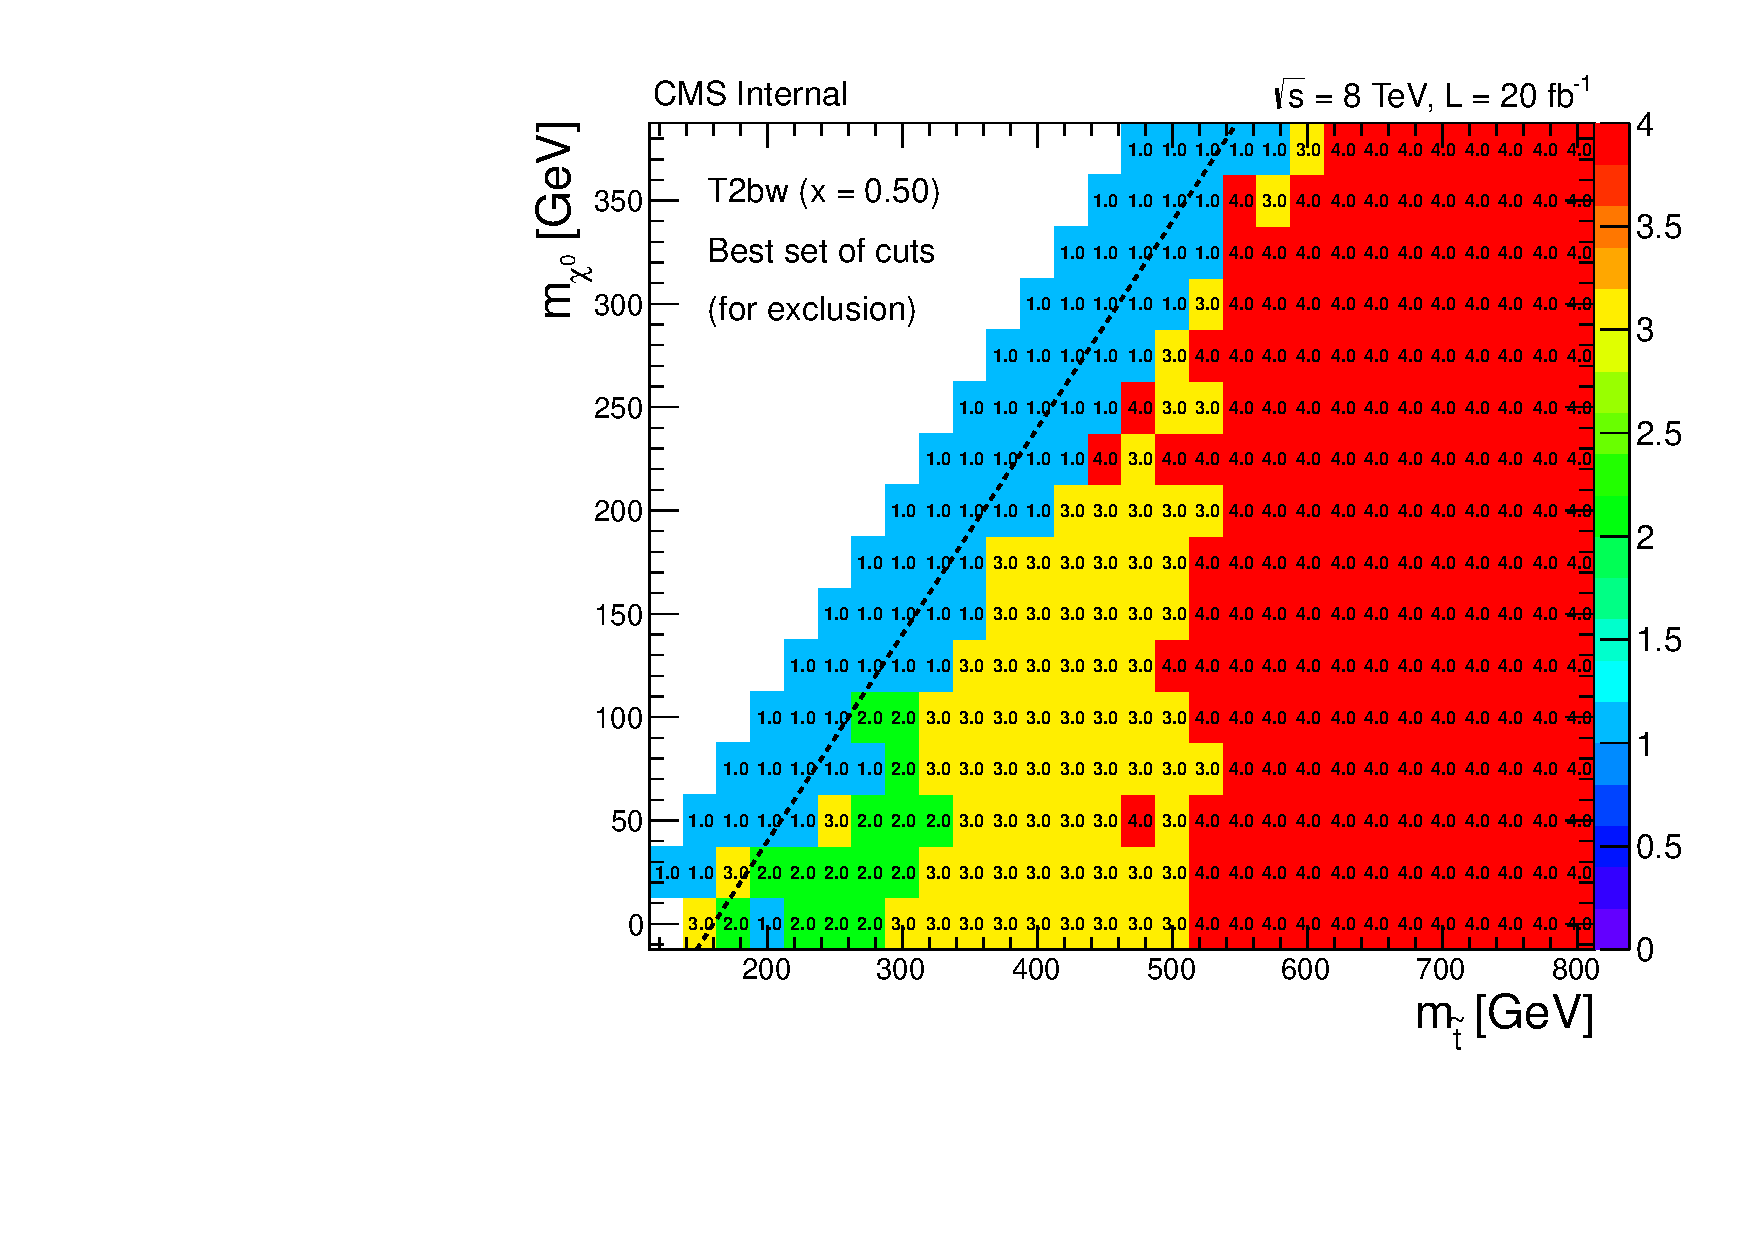
\includegraphics[width=0.37\textwidth]{cutAndCountPerformances/bestSet_T2bw050}
                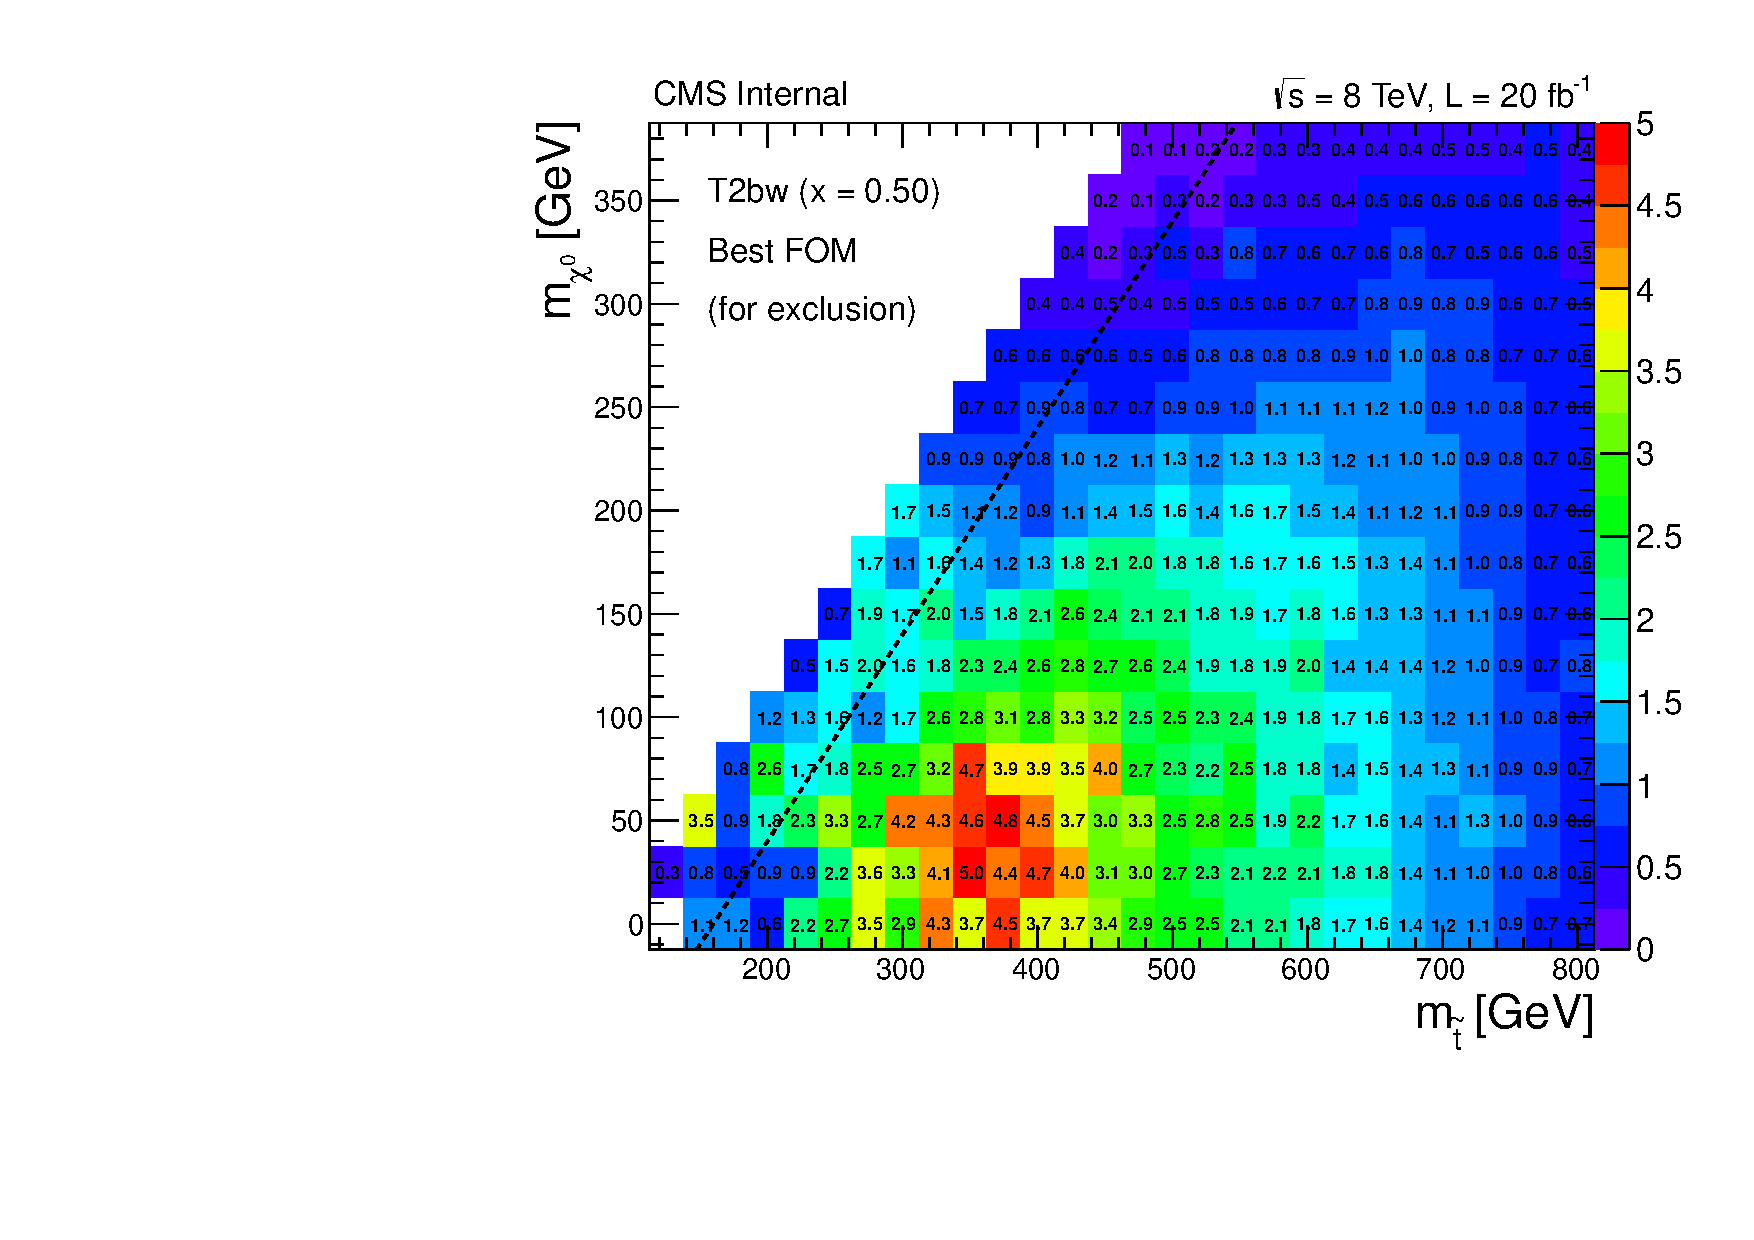
\includegraphics[width=0.37\textwidth]{cutAndCountPerformances/bestFOM_T2bw050}\\
                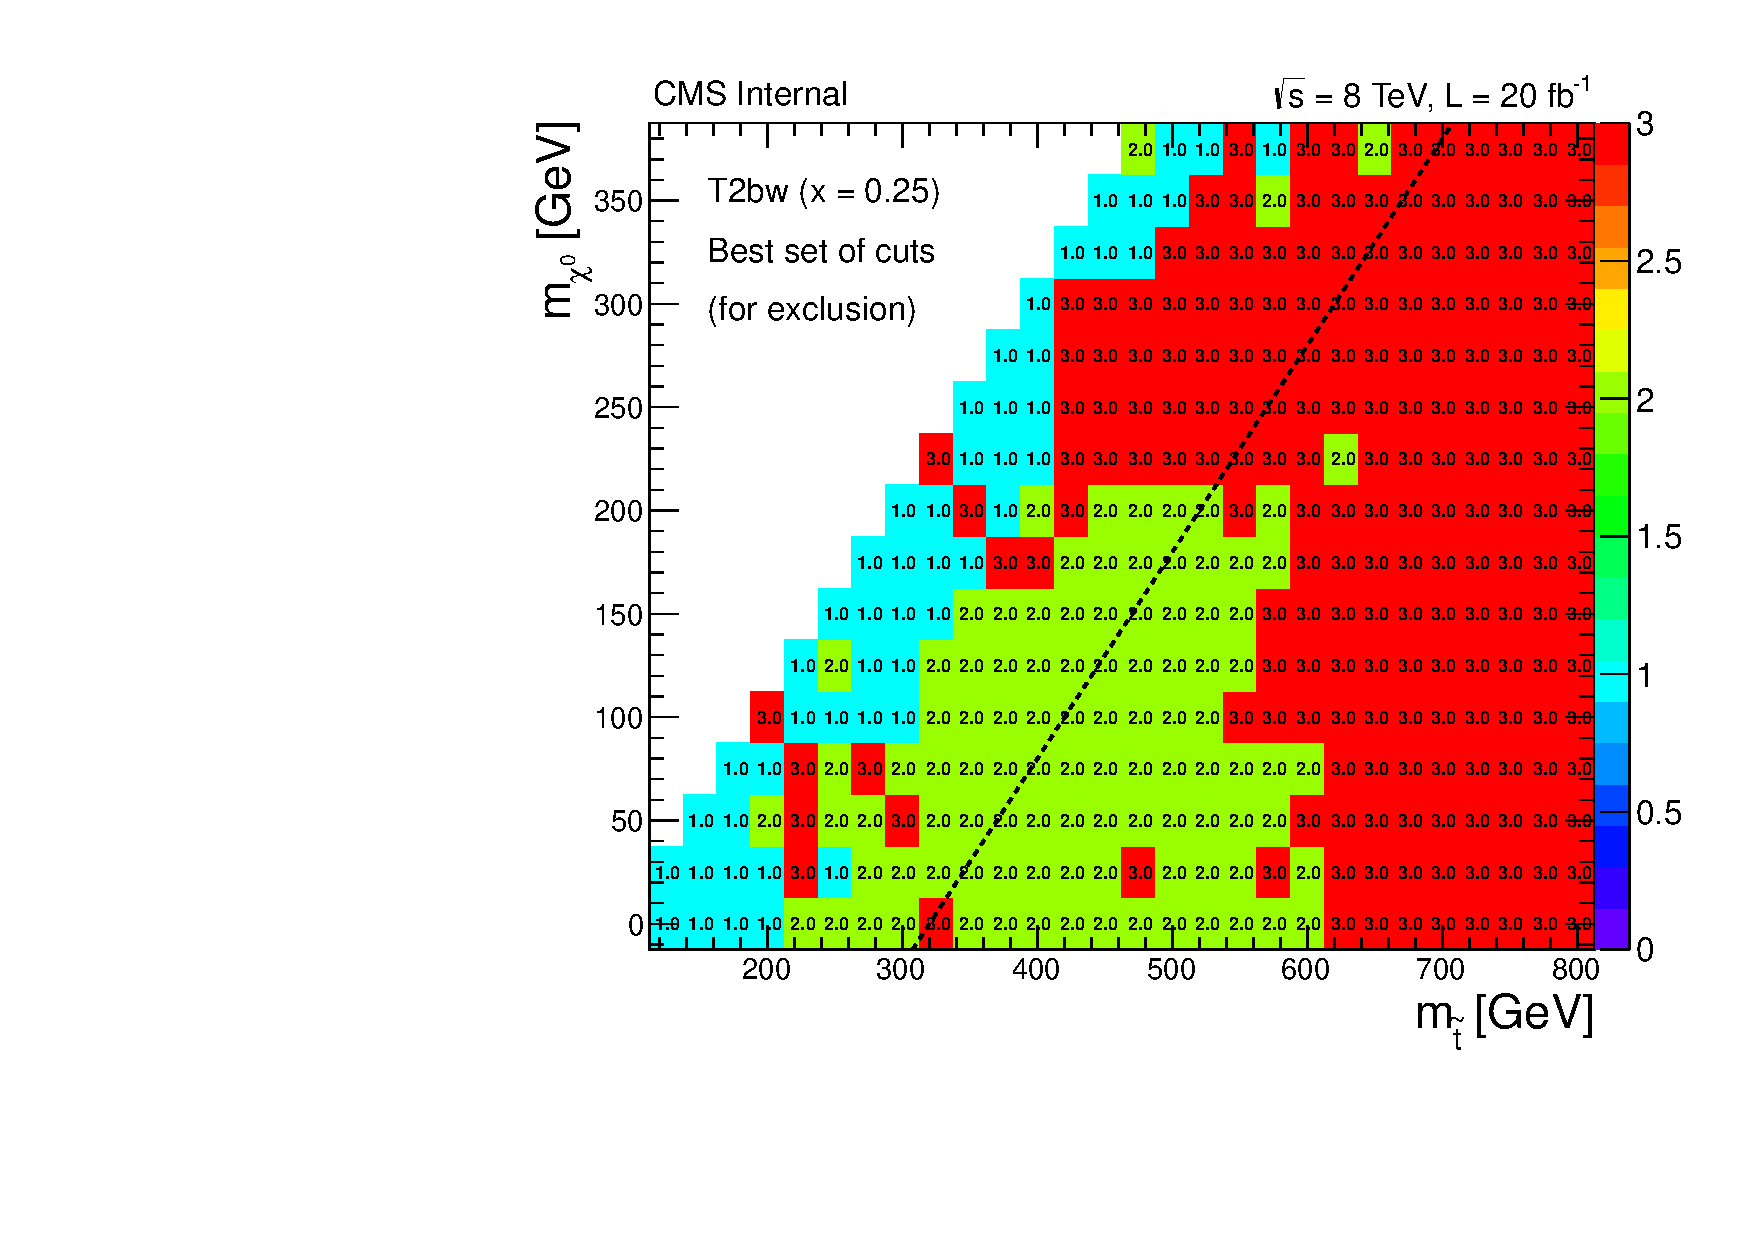
\includegraphics[width=0.37\textwidth]{cutAndCountPerformances/bestSet_T2bw025}
                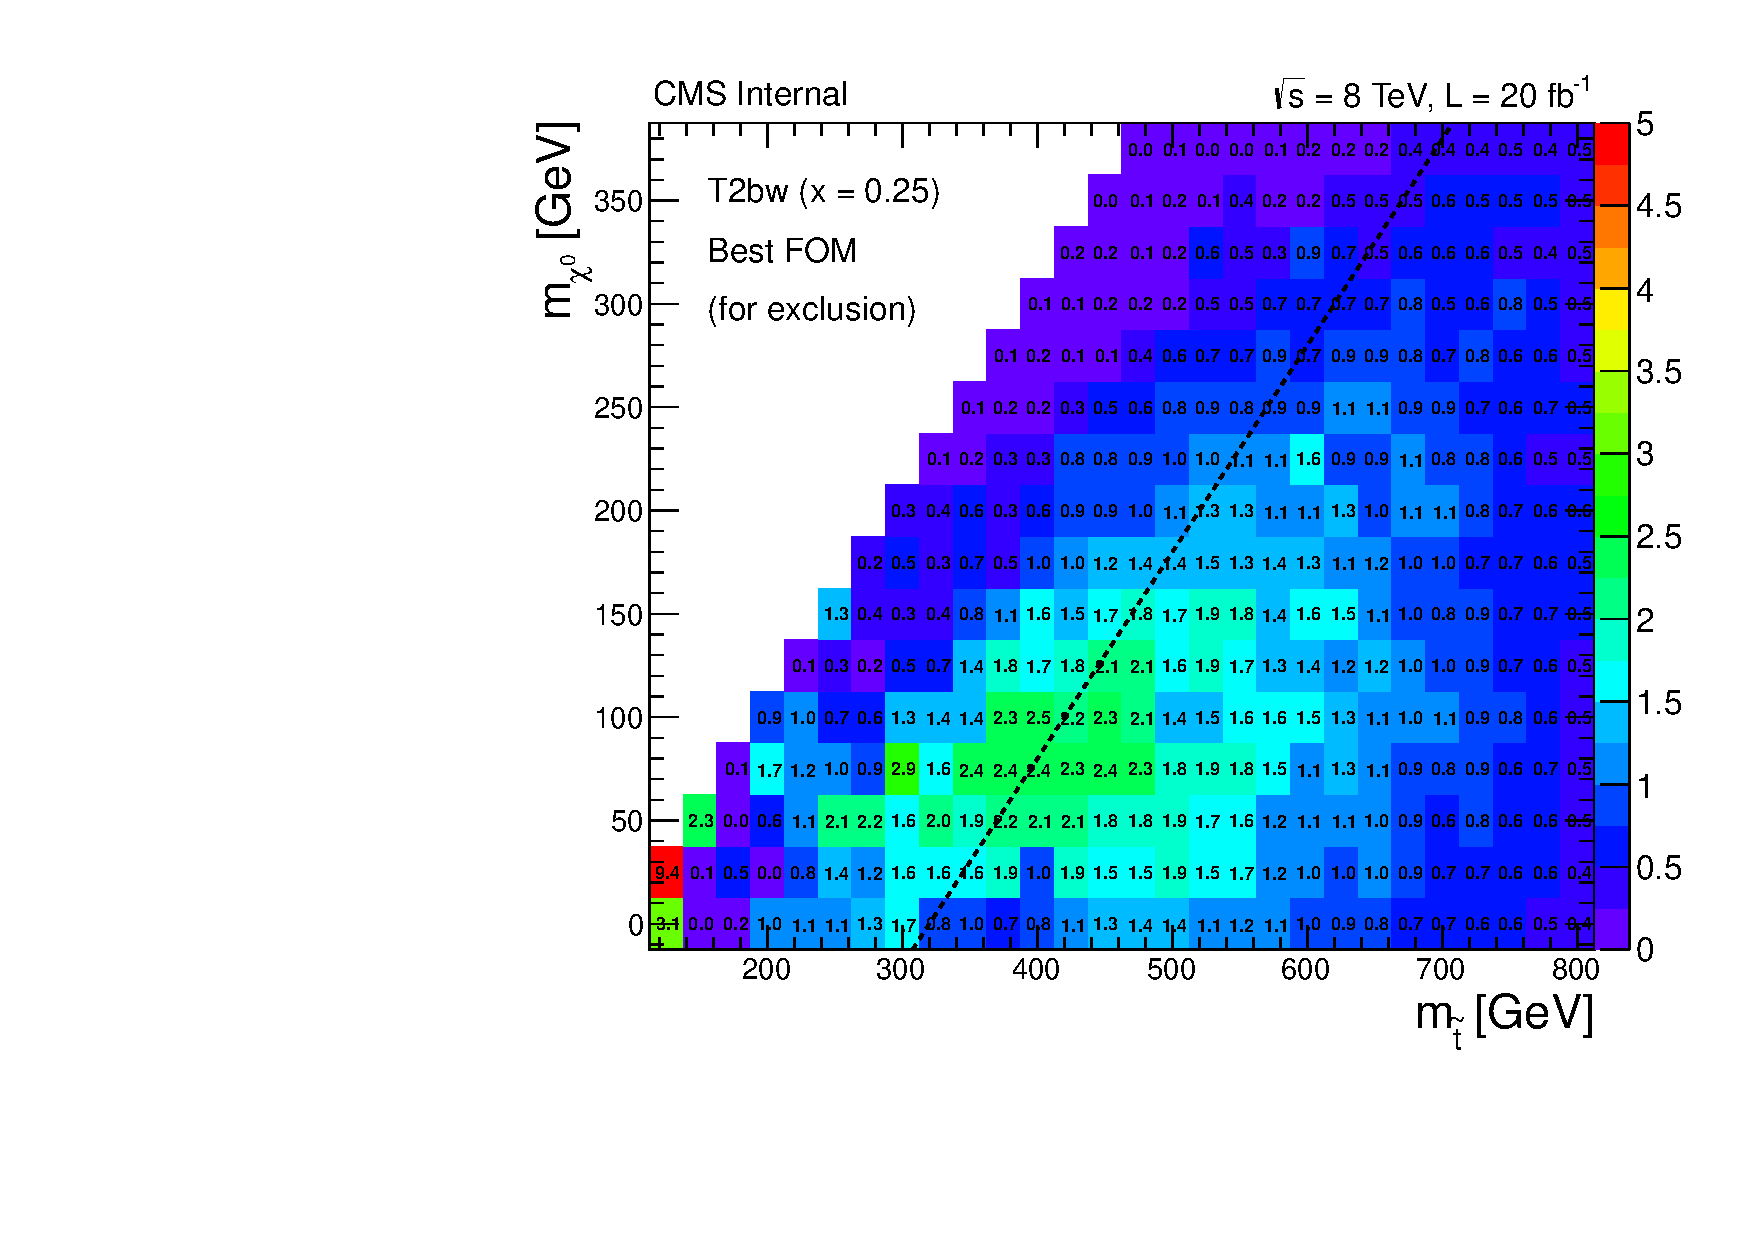
\includegraphics[width=0.37\textwidth]{cutAndCountPerformances/bestFOM_T2bw025}
                \caption{Best set of cuts (on the left) and performances in term of
                FoM$_\text{exclusion}$ (on the right) for the $\lstop \rightarrow t
                \lneutralino$ decay mode (first row) and $\lstop \rightarrow b \lchargino$
                decay mode with x = 0.75 (second row), 0.50 (third row) and 0.25 (last row).
                \todo{Maybe redo performance plot using the excluded signal strength formula+ contour at mu = 1, or if not show contour at FoM=2}}
                \label{fig:cutAndCountPerformances}
            \end{figure}

        \subsection{BDT-based signal regions}
        %==============================================================

        For the multivariate approach, several BDT are trained on slices of $\deltam$ in the $(\mass{\lstop},\mass{\lneutralino})$
        space against the $t\bar{t}$ background only. The choice of the variable is driven by an iterative method where variables
        are added to BDT and kept if the performances are overall significantly improved across different slices of $\deltam$. The
        performances of the BDTs are quantified by optimizing the cut on the BDT output with respect to a discovery-oriented
        FoM, considering all the backgrounds and assuming a relative systematic uncertainty of 15\%.

        The set of variables used are presented on Table \ref{tab:BDTVariableUsage} as function of the decay mode. The definition
        of the training region in the $(\mass{\lstop},\mass{\lneutralino})$ is then being looked at, noticing that some of the
        $\deltam$ slices can be merged together as the performances of the training are similar, essentially because the kinematic
        is not strongly different when moving from one slice to the other. The optimization of the cut on the BDT output is then
        performed by iteratively looking at the excluded cross-section after the full procedure explained in the following sections.
        The cuts are tuned manually to optimize the sensitivity accordingly. Here, because of the cross-section regimes leading to
        different amount of signal statistics, it is noticed that there is sometimes a significant gain in loosening or tightening
        the cut inside a same training region.

        The final definition of the training regions is presented on Figure \ref{fig:BDTTrainingRegions}. Each number represents a
        different BDT training. The dashed lines represent the cases when one training region leads to several cuts applied to define
        signal regions.

        \begin{table}[h!]
            \begin{center}
                \begin{tabular}{|c|cc|}

                    \hline
                    Variable                            & T2tt      & T2tt      \\
                                                        & off-shell & on-shell  \\
                    \hline
                    $\MET$                              & $\times$  & $\times$  \\
                    $H_{T}^\text{ratio}$                & $\times$  & $\times$  \\
                    $\pT(\text{lead. } \ell)$           & $\times$  & $\times$  \\
                    $\Delta\phi(j_{1,2},\vec{\MET})$    & $\times$  & $\times$  \\
                    $N_\text{jets}$                     & $\times$  & $\times$  \\
                    \hline
                    $\pT(\text{lead. jet})$             &           & $\times$  \\
                    $\Delta R( \ell, \text{lead. } b)$  &           & $\times$  \\
                    hadronic top $\chi^2$               &           & $\times$  \\
                    $M_{T2}^W$                          &           & $\times$  \\
                    $M_{\ell b}$                        & $\times$  &           \\
                    $\pT(\text{lead. } b)$              & $\times$  &           \\
                    \hline
                \end{tabular}
                \begin{tabular}{|c|ccc|}

                    \hline
                    Variable                            & T2bw      & T2bw      & T2bw      \\
                                                        & $x=0.25$  & $x=0.50$  & $x=0.75$  \\
                    \hline
                    $\MET$                              & $\times$  & $\times$  & $\times$  \\
                    $M_{T2}^W$                          & $\times$  & $\times$  & $\times$  \\
                    $M_{\ell b}$                        & $\times$  & $\times$  & $\times$  \\
                    $M_{3 b}$                           & $\times$  & $\times$  & $\times$  \\
                    $\pT(\text{lead. } \ell)$           & $\times$  & $\times$  & $\times$  \\
                    $\Delta\phi(j_{1,2},\vec{\MET})$    & $\times$  & $\times$  & $\times$  \\
                    $N_\text{jets}$                     & $\times$  & $\times$  & $\times$  \\
                    \hline
                    $\pT(\text{lead. } b)$              & $\times$  & $\times$  &           \\
                    $\Delta R( \ell, \text{lead. } b)$  &           & $\times$  &           \\
                    $H_{T}$                             &           &           & $\times$  \\
                    $\pT(\text{lead. jet})$             &           &           & $\times$  \\
                    \hline
                \end{tabular}
                \caption{List of variables considered for the training of the BDT
                as function of the decay mode. A $\times$ mark indicate that the variable
                is used in the final trainings.}
                \label{tab:BDTVariableUsage}
            \end{center}
        \end{table}

            \insertFourFigures{BDTTrainingRegions}
                              {BDT/training_T2tt}
                              {BDT/training_T2bw075}
                              {BDT/training_T2bw050}
                              {BDT/training_T2bw025}
                              {0.49}
                              {Slicing of the $(\mass{\lstop},\mass{\lneutralino})$ space
                              to define the training region of the BDTs. Some training
                              regions are subdivised into subregions where different cuts
                              are applied on the BDT output in order to adapt the sensitivity
                              to the local cross-section. \todo{Fix printability of plots}}

    \section{Background estimation \label{sec:analysis_backgroundEstimation}}
    %==============================================================

        \subsection{Overview}
        %==============================================================

    In this section, we focus on the estimation of the different background contributions.
    Four kinds of control regions are defined by inverting some of the requirements of the
    preselection and signal regions, as illustrated on Figure \ref{fig:backgroundEstimationOverview}.
    Each of these aim to provide signal-free sectors in which to check how good is the
    modeling of the backgrounds by the Monte-Carlo and perform data-driven estimations.

        \insertFigure{backgroundEstimationOverview}{0.7}
                     {Overview of the control regions used in the background estimation method. \todo{Fix printability of this sketch?}}

    The $\MT$-peak control region is defined by looking at events satisfying $50 < \MT <
    80\GeV$ instead of the signal region $\MT$ requirement. This control region is enriched
    in $\oneLeptonTop$ and is used as a well-controlled region in which to normalize the
    $\oneLeptonTop$, $\Wjets$ and $\diLeptonTop$ as documented in \ref{sec:MTpeakNormalization}.

    The $0\, b\text{-tag}$ control region is defined by requiring no $b$-tagged jet in the
    event. This region is enriched in $\Wjets$ and $\oneLeptonTop$ and is used to control
    and correct the tail of $\MT$ for these two components as described in \ref{sec:MTtailCorrection}.

    The $2\ell$ control region is defined by requiring exactly two selected leptons instead
    of one, at least one jet, and lowering the $\MET$ cut to $50 \GeV$. Additionnally, to limit the
    contribution from Drell-Yan, we veto events where the invariant mass of the dilepton
    system, $\mass{\ell\ell}$, is such that $\left|\mass{\ell\ell} - m_{Z}\right| < 15 \GeV$.
    Finally, the reversed veto control region is defined by requiring exactly one selected
    lepton and reversing the second lepton veto, effectively asking for an isolated track
    or $\tau$ as defined in \ref{sec:vetoLeptons}. This region  is intended to control
    the modeling of the second lepton veto. Both the $2\ell$ and reversed veto are being
    looked at on the whole $\MT$ range and are not used to derive scale factors but only
    systematic uncertainties on the background as detailed in \ref{sec:background_systematics}.

    Table \ref{tab:cutflowControlRegions} shows a breakdown of the background contributions
    in the different control regions at the preselection level.

\begin{table}[h!]
    \centering
\begin{tabular}{|c|cccc|}
    \hline
                     & $\MT$-peak       & $0\, b\text{-tag}$ ($M_T$ tail) & reversed veto    & 2 leptons             \\
    \hline
     $\oneLeptonTop$ & 18523 $\pm$ 55   &  1213 $\pm$ 14        &  7030 $\pm$ 34   &   41 $\pm$ 2.7  \\
     $\diLeptonTop$  &   656 $\pm$ 10   &   382 $\pm$ 8         &  7066 $\pm$ 34   & 9211 $\pm$ 39   \\
     $\Wjets$        &  1470 $\pm$ 24   &  2669 $\pm$ 33        &   331 $\pm$ 11   &  2.1 $\pm$ 0.9  \\
     rare            &  1209 $\pm$ 23   &   198 $\pm$ 7         &  1093 $\pm$ 20   &  626 $\pm$ 15   \\
    \hline
     total SM        & 21859 $\pm$ 66   &  4462 $\pm$ 38        & 15521 $\pm$ 53   & 9882 $\pm$ 42   \\
    \hline
\end{tabular}
    \caption{Breakdown of the yield of the different background categories in the four
    control regions without applying any signal region cuts. Uncertainties are statistical only.}
    \label{tab:cutflowControlRegions}
\end{table}

        \subsection{Background normalization in $\MT$-peak \label{sec:MTpeakNormalization}}
        %==============================================================

    The $\MT$-peak control region, defined as $50 < \MT < 80 \GeV$ is the first step of the
    background estimation method. It is used to normalize the $\oneLeptonTop$, $\Wjets$ and
    $\diLeptonTop$ components while the rare component is taken directly from Monte-Carlo.
    It is important to note that this normalization is done for each signal region individually,
    effectively allowing to absorb disagreements caused by cuts on not-so-well modeled
    variables and uncertainty on the jet energy scale, the trigger efficiency, the lepton
    identification efficiency and the luminosity.

    To separate the effect of the second lepton veto, the  normalization is done in two
    steps : first, a scale factor $\SFpre$ is computed before the application of the
    second lepton veto, substracting the rare component :

    \begin{equation}
        \SFpre \definedAs \left( \frac{N(\text{data}) - N(\text{rare})}{N(\oneLeptonTop) + N(\Wjets) + N(\diLeptonTop)} \right)
        \label{eq:SFpreDefinition}
    \end{equation}

    $\SFpre$ is used to normalize only the $\diLeptonTop$ component. Another scale factor,
    $\SFpost$ is used after application of the second lepton veto, substracting the rare
    and the corrected $\diLeptonTop$ component :

    \begin{equation}
        \SFpost \definedAs \left( \frac{N(\text{data}) - N(\text{rare}) - \SFpre \times N(\diLeptonTop)}{N(\oneLeptonTop) + N(\Wjets)} \right)
        \label{eq:SFpostDefinition}
    \end{equation}

     When applying no signal region cuts, $\SFpre$ and $\SFpost$ are equal to
     $(1.06 \pm 0.01)$ and $(1.05 \pm 0.01)$ respectively. This values, while not
     being compatible with 1, can be interpreted as a relatively small disagreement
     which is attributed to the misknowledge of the previously listed effects. Across the
     different cut-based signal regions, these scale factors range from $0.8$ to $1.4$,
     sometimes only compatible with unity at 3 standard deviations. The magnitude of this
     effect is attributed to bad modelization of the far tail of some variables in the
     Monte-Carlo.

        \subsection{$\MT$-tail correction in the $0\, b\text{-tag}$ region \label{sec:MTtailCorrection}}
        %==============================================================

    The $0\, b\text{-tag}$ control region allows to control the tail of $\MT$ for the $\Wjets$ and
    $\oneLeptonTop$ components. Before looking at the tail, however, we start by normalizing
    the background in the $\MT$ peak of this control region, in a similar fashion to what
    is done in \ref{sec:MTpeakNormalization}. This is done by introducing $\SFnobtag$,
    used to normalize the $\Wjets$ and $\oneLeptonTop$ contributions :

    \begin{equation}
        \SFnobtag \definedAs \left( \frac{N(\text{data}) - N(\text{rare}) - N(\diLeptonTop)}{N(\oneLeptonTop) + N(\Wjets)} \right)
        \label{eq:SF0btagDefinition}
    \end{equation}

    Without applying any signal cuts, $\SFnobtag$ is found to be $(0.99 \pm 0.01)$.
    After normalization to the peak, a clear disagreement in the tail of $\MT$ is observed
    for $\MT > 100 \GeV$ between the data and Monte-Carlo, as shown on Figure
    \ref{fig:templateFit/MT_notCorrected}. This is an important point of the analysis as
    it means that the Monte-Carlo needs to be corrected to have a reliable prediction of
    the $\oneLeptonTop$ and $\Wjets$ in the $\MT$ tail. \todo{Is it really a 'known'
    disagreement ... ? SMP-14-020, AN-2014/279 and AN-2014/114  see a disagreement
    for Wjets, but B2G-14-004 doesn't see anything for ttbar...}\todo{MTW sensitivity
    to MET also discussed in AN-15-013}.

    \insertFigure{templateFit/MT_notCorrected}{0.55}
                 {Data/MC comparison on the full $M_T$ distribution in the $0\, b\text{-tag}$ control
                 region at preselection level, after propagation of $\SFnobtag$. A clear
                 discrepancy is visible for $\MT > 100 \GeV$.}

    One can investigate the cause of the disagreement by first getting a better idea from
    the Monte-Carlo simulation of what is causing $\oneLeptonTop$ and $\Wjets$ events
    to each the tail of $\MT$. The resolution of $\MT$ is strongly related to both the
    resolution in $\pT$ of $\vec{\MET}$ and $\Delta\phi$ with the lepton. The relative
    resolution of $\MET$ and $\Delta \phi$ is investigated, defined as the ratio of the
    reconstructed quantity versus the generated quantity using only the generated
    neutrinos from the $W$ in the event. \todo{Maybe fix misleading 'resolution' name as here gen MET
    is only gen neutrino-MET...}. Figure \ref{fig:MTtailResolution} shows the distribution of the relative
    resolution of $\MET$ and $\Delta \phi$ as function of $\MT$ for the $\oneLeptonTop$
    background and its mean for each background.

    \insertFourFigures{MTtailResolution}
                      {MTtailResolution/MTvsMETReso}
                      {MTtailResolution/MTvsDeltaPhiReso}
                      {MTtailResolution/MTvsMeanMETReso}
                      {MTtailResolution/MTvsMeanDeltaPhiReso}
                      {0.45}
                      {$\MET$ and $\Delta \phi$ relative resolution as function of $\MT$,
                      using the generated $MET$ from neutrinos coming from a $W$, on top
                      showing the full 2 dimensional distribution and on bottom showing
                      the evolution of the mean resolution for each background. Error
                      bars corresponds to the uncertainties on the mean.}

    The results of this small investigation tends to point out that the $\MT$ tail for
    the $\oneLeptonTop$, $\Wjets$ and rare backgrounds originates more from the
    misreconstruction of the magnitude of the $\MET$ rather than it's direction. Small
    features are however observed in the $\Delta \phi$ spectra which can originate from
    other sources of $\MET$ in the event such as neutrinos inside $b$-jets.
    \todo{Complete this part later with results from Master students ?}

    %So far, the understanding of this disagreement comes from two source : first, the
    %off-shell contributions of $\Wjets$ is underestimated by the simulation, and second,
    %detector effects leads to a larger tail for the $\oneLeptonTop$ events.
    So far, the method used to correct the discrepancy is to compute ad-hoc scale factors
    using a template fit that estimate separately the contribution of $\oneLeptonTop$ and
    $\Wjets$ from the data. To do this, we use $\MlbPrime$ which was found to have a good
    discriminating power between the two process categories and being well discribed in
    the peak of $\MT$, as shown on Figure \ref{fig:MlbPrimeForTemplateFit}.

        \insertFourFigures{MlbPrimeForTemplateFit}
                          {templateFit/Mlb_0b_peak}
                          {templateFit/Mlb_0b_tail}
                          {templateFit/preselection_Mlb_noFit}
                          {templateFit/preselection_Mlb_withFit}
                          {0.45}
                          {Distribution of $\MlbPrime$ in the $0\, b\text{-tag}$ control region, data/MC comparison in the $M_T$ peak (top left), superimposed and normalized $\oneLeptonTop$ and $\Wjets$ components in the $M_T$ tail (top right), data/MC comparison in the $M_T$ tail before correction of the Monte-Carlo (bottom left) and after correction (bottom right). On the bottom right, the uncertainty of the scale factors are propagated in the ratio.}

    The method is implemented using the \textsc{RooFit} toolbox \refNeeded with the Minuit2
    implementation of the \textsc{Migrad} minimizer algorithm \refNeeded. The normalization
    of the $\oneLeptonTop$ and $\Wjets$ components are free parameters translated in term
    of scale factors, $SF_{\oneLeptonTop}$ and $SF_{\Wjets}$, while the normalization of
    the $\diLeptonTop$ and rare components are taken from the Monte-Carlo and constrained
    with a 20\% uncertainty during the fit process. To validate the method, a closure test
    is performed by generating toy data from the Monte-Carlo where arbitrary scale factors
    where injected. The estimated scale factors are then compared to the input scale factors.
    A very good linearity is found for scale factors varying from 0.10 to 3. The fit is
    performed both in the $\MT$ peak and tail regions and we extract $SFR = SF^{\text{tail}}
    / SF^{\text{peak}}$ for both processes, representing the discrepancy in the tail
    independently from the peak normalization. Different sources of systematic uncertainty
    are considered : the jet energy scale, the normalization of the rare background, the
    Monte-Carlo statistics, the choice of the minimizer algorithm, the choice of the
    initial fit conditions, the generator setup for $t\bar{t}$ (using \textsc{Powheg} or
    \textsc{MadGraph}, varying the matching parameters, RGE scale, top mass, applying or
    not the top $\pT$ reweighting). The most important sources are the Monte-Carlo statistics
    (leading to 11\% of relative uncertainty on SFR), the generator scale (9\%) and the jet
    energy scale. A conservative 20\% is used as relative systematic uncertainty.

    Without applying any signal region cuts, $\SFRoneLeptonTop$ and $\SFRWjets$ are found
    to be $(1.04 \pm 0.16 (\text{stat.}) \pm 0.21 (\text{syst.}))$ and $(1.33 \pm 0.10
    (\text{stat.}) \pm 0.27 (\text{syst.}) )$ respectively. The plot on Figure \ref{fig:MlbPrimeForTemplateFit}
    illustrate the impact on the $\MlbPrime$ data/MC comparison after propagating the scale
    factors. For the cut-based signal regions, we use the scale factors derived from a
    single $M_T$ cut associated to the signal region as shown on Figure \ref{fig:templateFit/CnC_MTcuts}.
    To cover possible correlation between the $SFR$ and $\MET$, the uncertainty from the
    single $\MET$ or $\MET/\sqrt{H_T}$ cut associated to the signal region is also
    quadratically added to the scale factor. These scale factors are shown on Figure \ref{fig:templateFitCnCResultsMET}.

    For the BDT signal regions, to be as close as possible to the kinematic of the BDT tails,
    we choose cuts on each BDT outputs such as at least 25\% of the background is still
    selected and apply the template fit method in that region. Two common scale factors
    to be applied to each BDT are then computed by averaging across all the trainings.
    The values found are $\SFRoneLeptonTop = (1.38 \pm 0.61)$ and $\SFRWjets = (1.21 \pm 0.36)$.

        \insertFigure{templateFit/CnC_MTcuts}
                     {0.6}
                     {Template fit results for individual cuts on $\MT$ after
                     preselection. The uncertainties shown are statistical only.}

        \insertTwoFigures{templateFitCnCResultsMET}
                         {templateFit/CnC_METcuts}
                         {templateFit/CnC_METoverSqrtHTcuts}
                         {0.45}
                         {Template fit results for invidiviual cuts on $\MET$ (left)
                         and $\MET/\sqrt{H_T}$ (right) after preselection + $\MT > 100\GeV$.
                         The uncertainties shown are statistical only.}

        \subsection{Control of $\diLeptonTop$ component and second lepton veto \label{sec:analysis_controlDileptonTop}}
        %==============================================================

        The 2-lepton and reversed veto control regions allow to check for the good modeling
        of the $\diLeptonTop$ background and the veto lepton definition. For the
        2 lepton control region, $\MT$ is defined using the leading lepton and ignoring
        the second one. The $\MT$-peak of the reversed veto control region is dominated by
        $\oneLeptonTop$ where a fake second lepton was reconstructed while the $\MT$-tail
        is dominated by $\diLeptonTop$ with a true second lepton. As for the $\MT$-peak
        normalization, we introduce scale factors to normalize the backgrounds in the peak
        of $\MT$ and quantify the agreement in the tail.

        In the reversed veto region, we define $\SFveto$ in a similar fashion as $\SFpost$,
        to control the fake-dominated region, and $\SFvetoTail$ to control the true second
        lepton dominated region after propagation of all the relevant scale factors including
        $\SFRoneLeptonTop$.

        Without applying any signal region cuts, we find $\SFveto = (1.18 \pm 0.03)$ and
        $\SFvetoTail = (1.07 \pm 0.02)$. The relatively large value of $\SFveto$ is
        interpreted as a mismodeling of the fake rate of the veto lepton by the Monte-Carlo
        and, despite being not compatible with unity, is not used to compute the prediction
        in the signal region because its effect is already included in $\SFpost$. The
        value of $\SFvetoTail$ also manifest a discrepancy in the veto lepton selection
        efficiency. Despite the fact that this scale factor is not propagated to the
        signal region, a systematic is later introduced to cover this effect.

        In the 2 leptons control region, we define $\SFtwoLep$ and $\SFtwoLepTail$ to
        control respectivelly the whole $\MT$ distribution and the tail of it.
        Without applying any signal region cuts, we find $\SFtwoLep = (0.96 \pm 0.01)$
        and $\SFtwoLepTail = (1.01 \pm 0.02)$ showing therefore a good modeling of $\MT$
        for this background.

        Another important check in the 2 leptons control region is the jet multiplicity
        modeling of $\diLeptonTop$ as the four jets requirements corresponds to two
        additional jets coming from radiations or pile-up for this background.
        Figure \ref{fig:} presents the distribution of the number of selected jets after
        application of $\MT>100$, which is found in good agreement.

        Figure \ref{fig:preselMT2leptonAndLepPlusVeto} presents the full $\MT$
        distributions for the reversed veto and two leptons control region.

        \begin{figure}[h!]
            \centering
            \includegraphics[width=0.45\textwidth]{controlPlots/reversedVeto_noMTCut/MT}
            \includegraphics[width=0.45\textwidth]{controlPlots/2leptons_noMTCut/MT}
            \caption{Full $\MT$ distributions for the reversed veto control region (on the left) and two leptons control region (on the right). On the left, $\SFpre$, $\SFveto$, $\SFRoneLeptonTop$ and $\SFRWjets$ are propagated. On the right, no scale factors is applied.}
                    \label{fig:preselMT2leptonAndLepPlusVeto}
        \end{figure}

        \insertFigure{controlPlots/2leptons/nJets}
                     {0.5}
                     {Distribution of the number of selected jets in the two leptons control region after applying $\MT > 100$.}

        \subsection{Control plots at preselection level}
        %==============================================================

        Figure \ref{fig:preselControlPlots} shows control plots for $\MT$, $\MET$ and $M_{T2}^W$ in the different control regions at the preselection level. \todo{Add comments here but I don't know what to say :/}

            \begin{figure}[h!]
                \centering
                \includegraphics[width=0.325\textwidth]{controlPlots/MTpeak/MT}
                \includegraphics[width=0.325\textwidth]{controlPlots/MTpeak/MET}
                \includegraphics[width=0.325\textwidth]{controlPlots/MTpeak/MT2W}\\
                \includegraphics[width=0.325\textwidth]{controlPlots/0btag/MT}
                \includegraphics[width=0.325\textwidth]{controlPlots/0btag/MET}
                \includegraphics[width=0.325\textwidth]{controlPlots/0btag/MT2W}\\
                \includegraphics[width=0.325\textwidth]{controlPlots/reversedVeto_noMTCut/MT}
                \includegraphics[width=0.325\textwidth]{controlPlots/reversedVeto_noMTCut/MET}
                \includegraphics[width=0.325\textwidth]{controlPlots/reversedVeto_noMTCut/MT2W}\\
                \includegraphics[width=0.325\textwidth]{controlPlots/2leptons_noMTCut/MT}
                \includegraphics[width=0.325\textwidth]{controlPlots/2leptons_noMTCut/MET}
                \includegraphics[width=0.325\textwidth]{controlPlots/2leptons_noMTCut/MT2W}\\
                \caption{A few control plots, showing the data/MC comparison for $\MT$ (left column),
                        $\MET$ (middle column) and $M_{T2}^W$ (right column) in the different control
                        regions : $\MT$-peak (first row), $0\, b\text{-tag}$ (second row), reversed veto (third
                        row) and 2 leptons (fourth row). The $\MT$-peak normalization and $\MT$-tail
                        correction scale factors are propagated where relevant.}
                        \label{fig:preselControlPlots}
            \end{figure}

        \subsection{Background prediction}
        %==============================================================

        The background prediction is obtained by taking the Monte-Carlo yield in the
        $\MT$-tail and propagating $\SFpre$ to the $\diLeptonTop$ component and $\SFpost$
        to the $\oneLeptonTop$ and $\Wjets$ component. The $\oneLeptonTop$ and $\Wjets$
        are also corrected with $\SFRoneLeptonTop$ and $\SFRWjets$ respectively. The
        prediction for the rare component is directly the Monte-Carlo yield in $\MT$-tail.
        The formula \ref{eq:prediction1ltop} to \ref{eq:predictionrare} below summarize
        the computation of the prediction. The procedure is repeated for each signal
        region as all the scale factors involved are signal-region dependent. As an
        illustration, Table \ref{tab:predictionPreselection} shows the comparison between
        the raw Monte-Carlo and the prediction obtained at preselection level.

        \begin{eqnarray}
            N^\text{pred}_\text{tail}(\oneLeptonTop) & = & N^\text{MC}_\text{tail}(\oneLeptonTop)  \times \SFpost \times \SFRoneLeptonTop \label{eq:prediction1ltop}  \\
            N^\text{pred}_\text{tail}(\Wjets)        & = & N^\text{MC}_\text{tail}(\Wjets)         \times \SFpost  \times \SFRWjets                             \\
            N^\text{pred}_\text{tail}(\diLeptonTop)  & = & N^\text{MC}_\text{tail}(\diLeptonTop)   \times \SFpre                                                \\
            N^\text{pred}_\text{tail}(\text{rare})   & = & N^\text{MC}_\text{tail}(\text{rare})                                           \label{eq:predictionrare}
        \end{eqnarray}

        \begin{table}[!h]
            \begin{center}
                \begin{tabular}{|l|c|c|}
                    \hline
                                             &  \textbf{Raw MC}    & \textbf{Prediction}       \\
                    \hline
                    \textbf{$\oneLeptonTop$} &  5970 $\pm$ 31      & 6526 $\pm$ 1632     \\
                    \textbf{$\diLeptonTop$}  &  2117 $\pm$ 18      & 2253 $\pm$  229     \\
                    \textbf{$\Wjets$}        &   477 $\pm$ 13      &  669 $\pm$  364     \\
                    \textbf{rare}            &   490 $\pm$ 13      &  490 $\pm$  245     \\
                    \hline
                    \textbf{Total SM}        &  9055 $\pm$ 41      & 9940 $\pm$ 1666     \\
                    \hline
                \end{tabular}
                \caption{ Background prediction at the preselection + $\MT > 100\GeV$ level.}
                \label{tab:predictionPreselection}
            \end{center}
        \end{table}

    \section{Systematic uncertainties \label{sec:analysis_systematics}}
    %==============================================================

        This section describes the sources of systematics uncertainties that are considered for the background and the signal.

        \subsection{Systematic uncertainties on the background \label{sec:background_systematics}}
        %==============================================================

            Several sources of systematic uncertainties are considered for the background,
            the most important ones being from the $\MT$-peak normalization, the $\MT$-tail
            correction and the $\diLeptonTop$ modeling of the $\MT$ tail.

            \subsubsection{Modeling of $\diLeptonTop$ in $\MT$ tail}

            As discussed in section \ref{sec:analysis_controlDileptonTop}, the modeling by
            the Monte-Carlo of the $\MT$ tail of the $\diLeptonTop$ background is found
            to be good in the 2 leptons and reversed veto control regions. As it is a
            major background of the analysis, a systematic uncertainty is nevertheless
            asserted to quantify the trust in the Monte-Carlo on a per-signal-region basis.

            To do this, one wants to probe the 2 leptons and reversed veto control regions
            as close as possible of the signal region. However, as the signal region cuts
            are sometimes quite tight, the remaining statistics in these control region is
            too low and doesn't allow a reasonnable check of the distributions. To work
            around this problem while still probing the tail of $\MT$ near the signal
            region, we define loosened cuts to check these scale factors with more
            statistics. These cuts are designed by requiring to have at least 30 events
            remaining in the tail of $\MT$ for the 2 lepton control region.

            For each of the relaxed control region, we compute the value of $\SFtwoLepTail$
            and $\SFvetoTail$ to quantify the agreement between data and the simulation in
            the tail of $\MT$. An enveloppe is then computed computed for each signal
            region to account for the spread of the scale factors for each of the
            associated control regions. For the cut-based signal regions, this lead to a
            relative uncertainty on the total yield varying from 1.5 to 35\%. For the
            BDT signal regions, this relative uncertainty is between 7 and 40\%.

            \subsubsection{Second lepton veto efficiency}
            %============================================

            The uncertainty on the efficiency of the second lepton veto is propagated to the
            fraction of $\diLeptonTop$ events that have a second lepton in the acceptance. For
            the isolated track veto lepton, this is defined as having a second generated
            $e/\mu$ or a one prong $\tau \rightarrow h$ with $\pT > 5 \text{ or } 10 \GeV$,
            respectively, with $\abseta < 2.4$. This fraction is between 50-70\% for all
            signal regions. The uncertainty for these events is 6\% and is obtained from
            tag-and-probe studies \refNeeded. Regarding the $\tau$ veto leptons, the
            events considered are those with a hadronic $\tau$ in the acceptance, with
            true visible transverse energy $> 20\GeV$ in $\abseta < 2.4$. This fraction is
            about $10 \sim 20 \%$ of the total. The uncertainty on the efficiency of the
            $\tau$-ID algorithm is 7\%, taken from $\tau$ group studies \refNeeded.

            \subsubsection{Uncertainty on $\SFRoneLeptonTop$ and $\SFRWjets$}
            %================================================================

            As described in section \label{sec:MTtailCorrection}, the $\MT$-tail correction
            scale factors for $\oneLeptonTop$ and $\Wjets$ are computed with an uncertainty
            coming from statistics in the $0\, b\text{-tag}$ control region and systematic effects
            from the template fit method itself, as well as . This uncertainty is propagated
            to the total background yield uncertainty and is one of the major contribution
            for the signal region with a large remaining fraction of $\oneLeptonTop$.
            For the cut-based signal regions, this corresponds to a relative uncertainty
            on the total background ranging from 0 to 15\% and up to 17\% for the BDT
            signal regions.

            \subsubsection{Statistic uncertainty in $\MT$ peak}
            %==============================================================

            The $\MT$-peak normalization scale factors are an important part of the background
            estimation procedure, but is nevertheless limited by the statistics available
            in the peak region. Therefore, the $\SFpre$ and $\SFpost$ scale factors come
            associated to an uncertainty, dominated by the event count of data. This
            uncertainty is propagated to the prediction in the tail. This lead to a
            relative uncertainty on the total background ranging from 2 to 15\% for the cut-based
            signal regions and between 3 and 40\% for the BDT signal regions.

            \subsubsection{Other sources of systematic uncertainties}
            %========================================================

            Other sources of uncertainties are taken into account though being small compared
            to the ones described in the previous subsections :
            \begin{itemize}
                \item To cover the modeling of of ISR and FSR jets, the $N_\text{jets}$
                      distribution is studied in the 2 leptons control region. An
                      uncertainty of 2\% is asserted on the $\diLeptonTop$ background
                      from this check.
                \item To account for possible mismodeling of the relative proportions of
                      the backgrounds, the $\oneLeptonTop$ component cross-section
                      is varied by 10\% while the $\Wjets$ cross-section is varied by 50\%
                      during the background estimation procedure.
                \item As the rare category is quite difficult to estimate because composed
                      of a large number of background, its contribution is taken directly
                      from MC. We however put a conservative 50\% uncertainty in the
                      rate of this category.
                \item The Monte-Carlo statistics available in the $\MT$ tail being limited,
                      it also contributes to the systematic uncertainty on the final prediction.
            \end{itemize}

            \subsubsection{Summary of background uncertainties at preselection}
            %==============================================================

            Table \ref{tab:systematicSummary} shows a breakdown of the different systematics
            uncertainties that are considered, at preselection level and the range of them
            for the two kinds of signal regions. The relative importance of the individual
            systematics varies depending of the signal regions as the composition of the
            background itself varies : at preselection level, the importance of the
            $\SFRoneLeptonTop$ uncertainty is high as the $\oneLeptonTop$ component is still large.
            However for some signal regions, the $\diLeptonTop$ is the dominant contributions and
            uncertainty from the $\MT$-tail modeling is the leading systematic source.

            % Add range of uncertainties in the signal regions

            \begin{table}[!ht]
                \begin{center}
                    \begin{tabular}{|l|c|cc|}
                        \hline
                                                                       & Preselection    & Cut-based      & BDT             \\
                                                                       & + $\MT>100\GeV$ & signal regions & signal regions  \\
                        \hline
                        \textbf{$\diLeptonTop$ ($\MT$-tail modeling)}  & 1.6                      & 2-35         & 7-40    \\
                        \textbf{$\diLeptonTop$ (jets modeling)}        & 1.1                      & 1-4          & 0.5-4   \\
                        \textbf{$\diLeptonTop$ (2nd lepton veto)}      & 1.2                      & 0-4          & 1-4     \\
                        \textbf{$\SFRWjets$ uncertainty}               & 1.4                      & 0-6          & 0-5     \\
                        \textbf{$\SFRoneLeptonTop$ uncertainty}        & 16.4                     & 0-15         & 0-17    \\
                        \textbf{$\MT$-peak SF uncertainties}           & 0.7                      & 2-15         & 3-40    \\
                        \textbf{Cross-sections and MC stat}            & 1.9                      & 7-48         & 7-47    \\
                        \hline
                        \textbf{total}                                 & 16.8                     & 12-50        & 25-60   \\
                        \hline
                    \end{tabular}
                    \caption{Summary of the relative uncertainties at preselection+$\MT>100\GeV$
                    and range of relative uncertainties with respect to the total predicted
                    background yield for cut-based signal regions and BDT signal regions.
                    \label{tab:systematicsSummary}}
                \end{center}
            \end{table}

        \subsection{Systematic uncertainties on the signal}
            %==============================================================

        While the background prediction is dominated by data-driven systematic
        uncertainties, the signal uncertainty sources are more related to the
        confidence in the different element of the construction of the Monte-Carlo
        samples and algorithm used.

        The limited available statistics of the signal sample leads to a 2\% maximal
        2\% uncertainty. The integrated luminosity is known with a precision of 2.2\%
        and is propagated to the uncertainty of the yield. The trigger efficiency
        used in the very first steps of the selection is known with a precision of 3\%.
        The lepton identification and isolation efficiency are observed to be consistent
        between data and Monte-Carlo within an envelope of 5\%.

        The jet energy scale uncertainty is studied by varying the jet energy corrections
        within their $\pm$1 sigma uncertainty before the jet selection. The variation is
        properly propagated into the $\MET$ value. During the process, we also assume a
        10\% uncertainty on the unclustered energy defined as $(\vec{\MET} + \sum_\text{jets}
        \vec{p} + \sum_\text{leptons} \vec{p})$ where jets and leptons are selected with looser
        $\pT$ and $\abseta$ requirements. This effect leads to a maximum 10\% uncertainty on
        the signal yields.

        The uncertainty on the reshaping of the $b$-tagging discriminator is also considered
        by varying the technique within $\pm$1 sigma uncertainy before the application of
        $b$-tagging requirements. This leads to a 3\% uncertainty on the signal yields.

        The uncertainty on the ISR jets reweighting applied on signal is taken from data/MC
        scale factors derived from the analysis of events with high $\diLeptonTop$ purity. The
        scale factors, function of the $\pT$ recoil of the system, are varied within their
        uncertainties and lead to a maximum variation of 8 and 10\% on the signal yield, depending
        of the decay mode.

        Finally, the uncertainty on PDF are calculated, following the PDF4LHC prescription,
        using the CT10, NNPDF 2.1, and MSTW2009 PDF sets. \refNeeded The impact on the
        signal efficiency range from 10 to 30\% depending of the signal mass point.

    \section{Signal contamination handling}
    %==============================================================

        Signal contamination occurs when a significant fraction of signal events is present in
        the control regons. While it doesn't affect the predicted yield for the background-only hypothesis
        ($H_0$), a significant contamination can bias the data-driven aspects of the background
        estimation when predicting the expected yield under the signal hypothesis ($H_1$). As a
        consequence, it leads to an overestimation of the expected background under the signal hypothesis
        therefore increasing the probability to incorrectly reject the signal hypothesis (type II error).

        The signal contamination level is studied across the $(\mass{\lstop},\mass{\lneutralino})$
        plane by computing the $C \definedAs S/B$ in the $\MT$-peak control region and 0 $b$-tag
        control region and comparing it to the signal purity, $P \definedAs S/B$, in the signal region :

        \begin{equation}
            R \definedAs \frac{C}{P} = \frac{(S/B)_\text{control region}}{(S/B)_\text{signal region}}
            \label{eq:contaminationRatio}
        \end{equation}

        This ratio $R$ is found to be sometimes higher than an arbitrary treshold value of 15$\sim$20\%.
        This is especially true when considering the the low $\deltam$ region of the $(\mass{\lstop},
        \mass{\lneutralino})$ plane, as the signal is likely to get smaller values of $\MT$ and the $b$-jets
        are less likely to be selected or correctly $b$-tagged as their momentum decrease. This is illustrated
        on Figure \ref{fig:signalContaminationIllustration} which shows the differences in shape of $\MT$ and
        $b$-tagged jet multiplicity for two benchmarks of the $\lstop \rightarrow t \lneutralino$ decay mode.

        \insertTwoFigures{signalContaminationIllustration}
                         {signalContamination/MT}{signalContamination/nBtag}{0.4}
                         {Illustration of the signal contamination evolution using two signal example :
                         T2tt (250/100) has 30\% of events with 0$b$-tag jets and a large fraction of events at low $\MT$.}

        It is concluded that the signal contamination can not be neglected. One needs to correct the modeling
        of the $H_1$ hypothesis by peforming a different background estimation $\tilde{B}$ compared to the
        $H_0$ hypothesis.

        The data-driven aspects are corrected by including the signal when computing the scale factors for the
        $\MT$-peak normalization and $\MT$-tail correction. In the case of $\SFpre$ and $\SFpost$, the scale factors
        are corrected by substracting both the rare and signal component to normalize the $\oneLeptonTop$, $\Wjets$
        and $\diLeptonTop$ components :

        \begin{equation}
            \SFpreTilde \definedAs \left( \frac{N(\text{data}) - N(\text{rare} - N(\text{signal}))}{N(\oneLeptonTop) + N(\Wjets) + N(\diLeptonTop)} \right)
        \end{equation}
        \begin{equation}
            \SFpostTilde \definedAs \left( \frac{N(\text{data}) - N(\text{rare}) - N(\text{signal}) - \SFpreTilde \times N(\diLeptonTop)}{N(\oneLeptonTop) + N(\Wjets)} \right)
        \end{equation}

        In the case of the $\MT$-tail correction scale factors, they are corrected by including the signal contribution
        to the rare category before fitting the $\oneLeptonTop$ and $\Wjets$ components to the data using the template
        fit method. We however constrain a posteriori to the fit $\SFRoneLeptonTopTilde$ to be $\geq 1$.

        The corrected background $\tilde{B}$ is computed the same way as described in equations \ref{eq:prediction1ltop} to \ref{eq:predictionrare}
        using the corrected scale factors. As the correction depends of the signal, it is shall be performed on a per-benchmark
        basis. However, as it is a CPU intensive task, it is done only with a setp of $50 \GeV$ instead of the $25 \GeV$
        of the signal samples. The background prediction for other benchmarks is corrected using an interpolation of
        the ration $\tilde{B}/B$ across the $(\mass{\lstop},\mass{\lneutralino})$ plane. Figure \ref{fig:signalContaminationSFmap} shows
        the obtained ratio $\tilde{B}/B$ for each signal type, showing an effect up to 25\% at low masses.

        \insertFourFigures{signalContaminationSFmap}
                          {signalContamination/globalSFmap_T2tt}
                          {signalContamination/globalSFmap_T2bw-075}
                          {signalContamination/globalSFmap_T2bw-050}
                          {signalContamination/globalSFmap_T2bw-025}
                          {0.4}
                          {Map of the ratio $\tilde{B}/B$, i.e. signal-contamination corrected background prediction versus uncorrected prediction, using the BDT signal regions and for the $\lstop \rightarrow t \lneutralino$ decay mode (top left) and $\lstop \rightarrow b \lchargino$ decay mode with $x=0.75$ (top right), $x=0.50$ (bottom left) and $x=0.25$ (bottom right).}

    \section{Results and interpretation \label{sec:analysis_results}}
    %==============================================================

    On the left of figures \ref{fig:resultsCnC} and \ref{fig:resultsBDT}, comparisons
    of the yield between data and background prediction under the null hypothesis
    for each signal regions of the cut-based approach and BDT approach are presented.
    A good compatibility is observed with the background-only expectation. The results
    are therefore interpreted in terms of upper limit on $\sigma{\lstop\lstop} \times BR$
    with a 95\% confidence level.  Comparing the upper limit with the theoretical
    expectation for a branching ratio of 1, one can derive limits in terms of excluded
    region of the $(\mass{\lstop}, \mass{\lneutralino})$ space, as reported on the right
    of figures \ref{fig:resultsCnC} and \ref{fig:resultsBDT}. During the interpretation,
    the signal hypothesis modeling is corrected to account for signal contamination.

    \begin{figure}[h!]
        \centering
        \includegraphics[width=0.33\textwidth]{results/CnC_T2tt/signalRegion_MTtail_yield}
        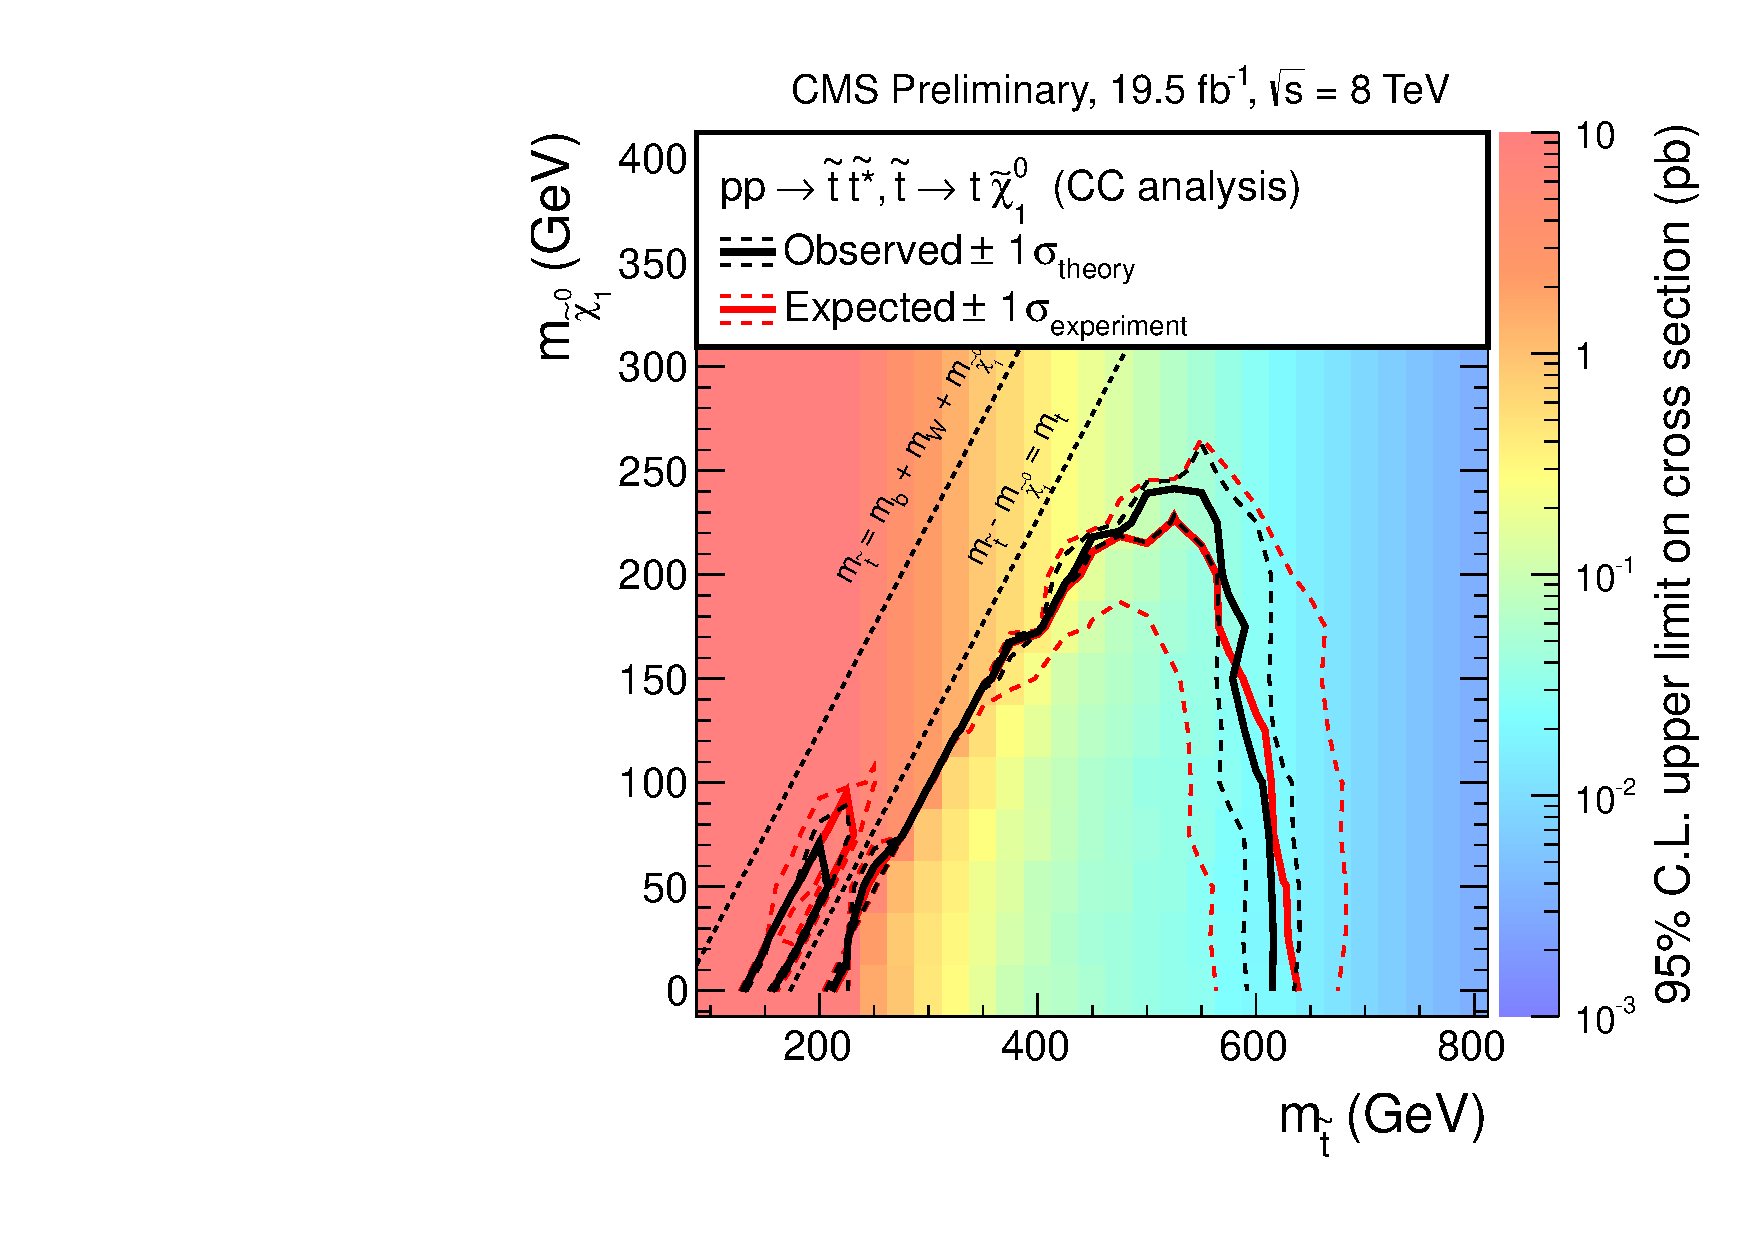
\includegraphics[width=0.31\textwidth]{limits/T2tt_CC}\\
        \includegraphics[width=0.33\textwidth]{results/CnC_T2bw075/signalRegion_MTtail_yield}
        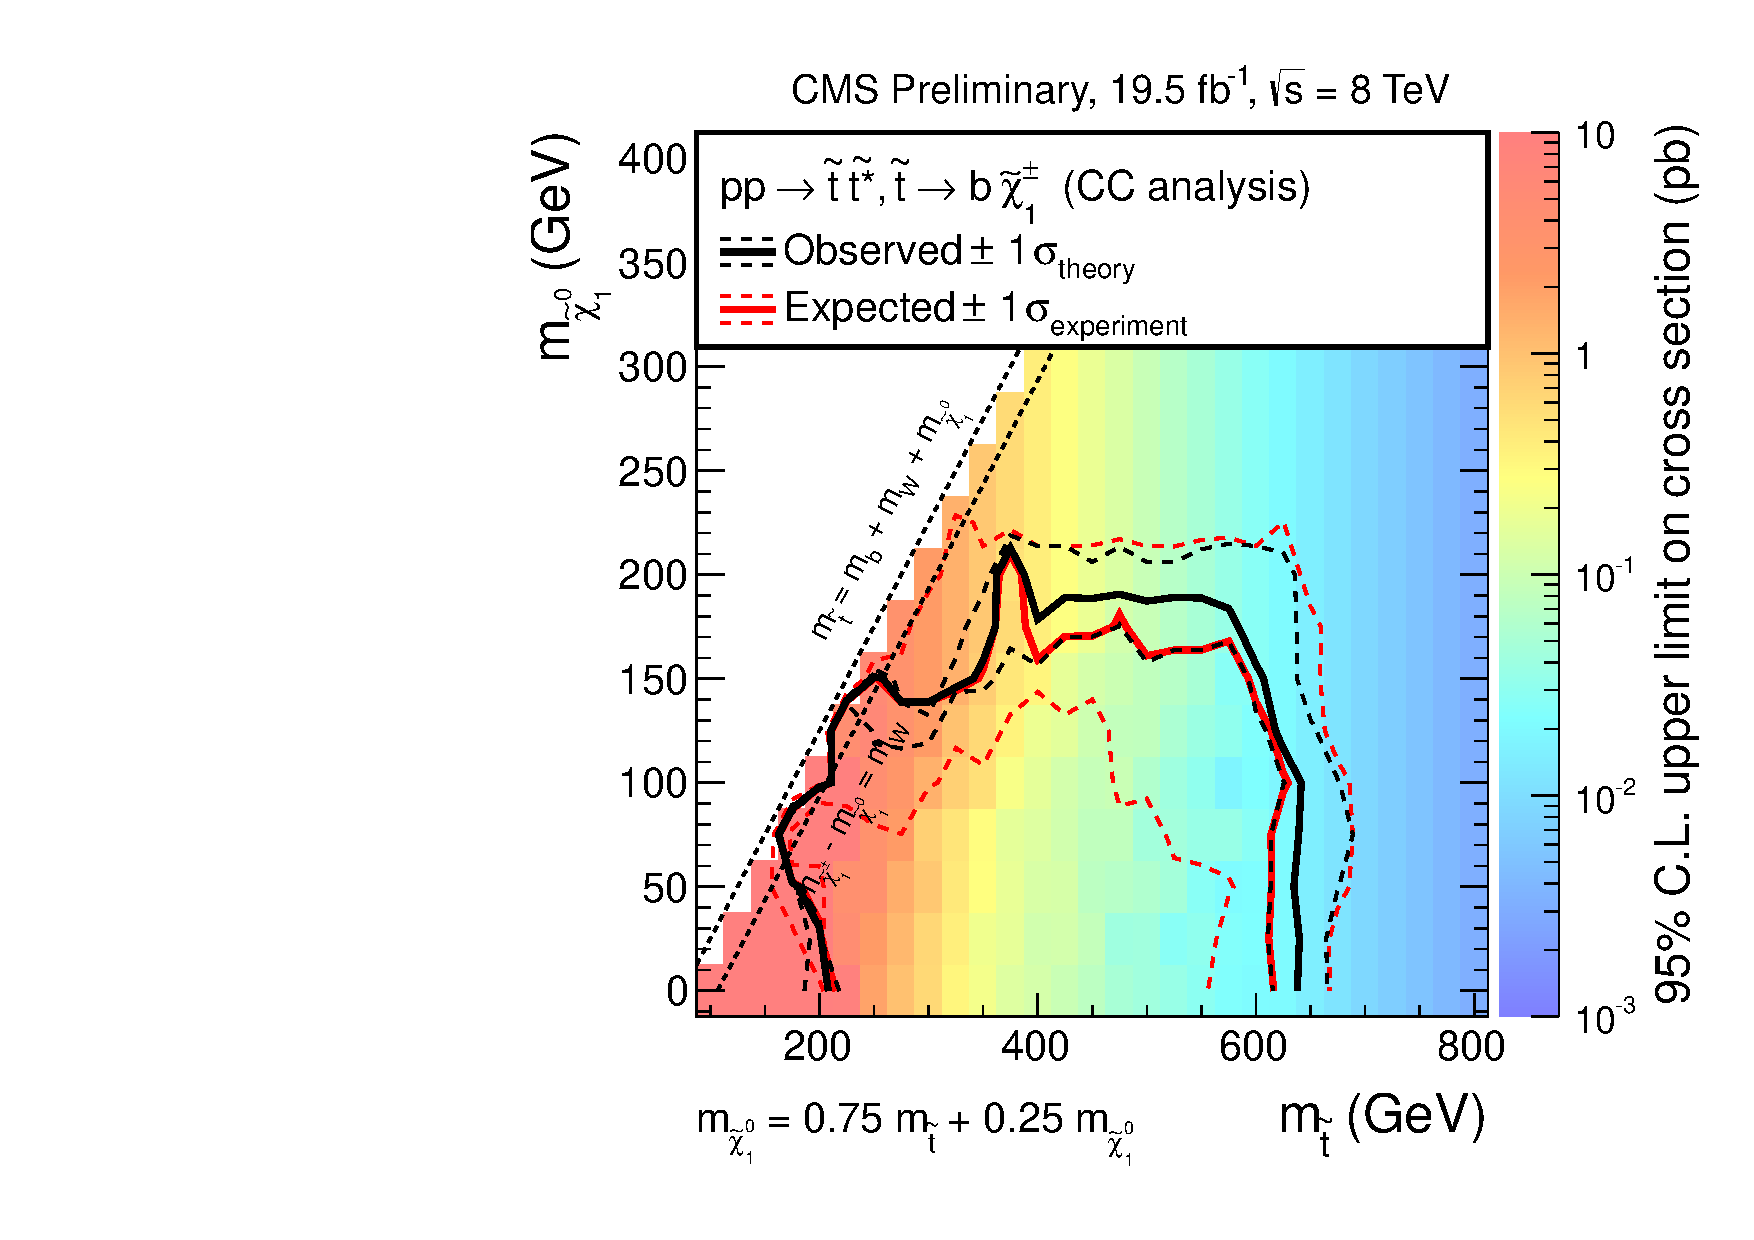
\includegraphics[width=0.31\textwidth]{limits/T2bw075_CC}\\
        \includegraphics[width=0.33\textwidth]{results/CnC_T2bw050/signalRegion_MTtail_yield}
        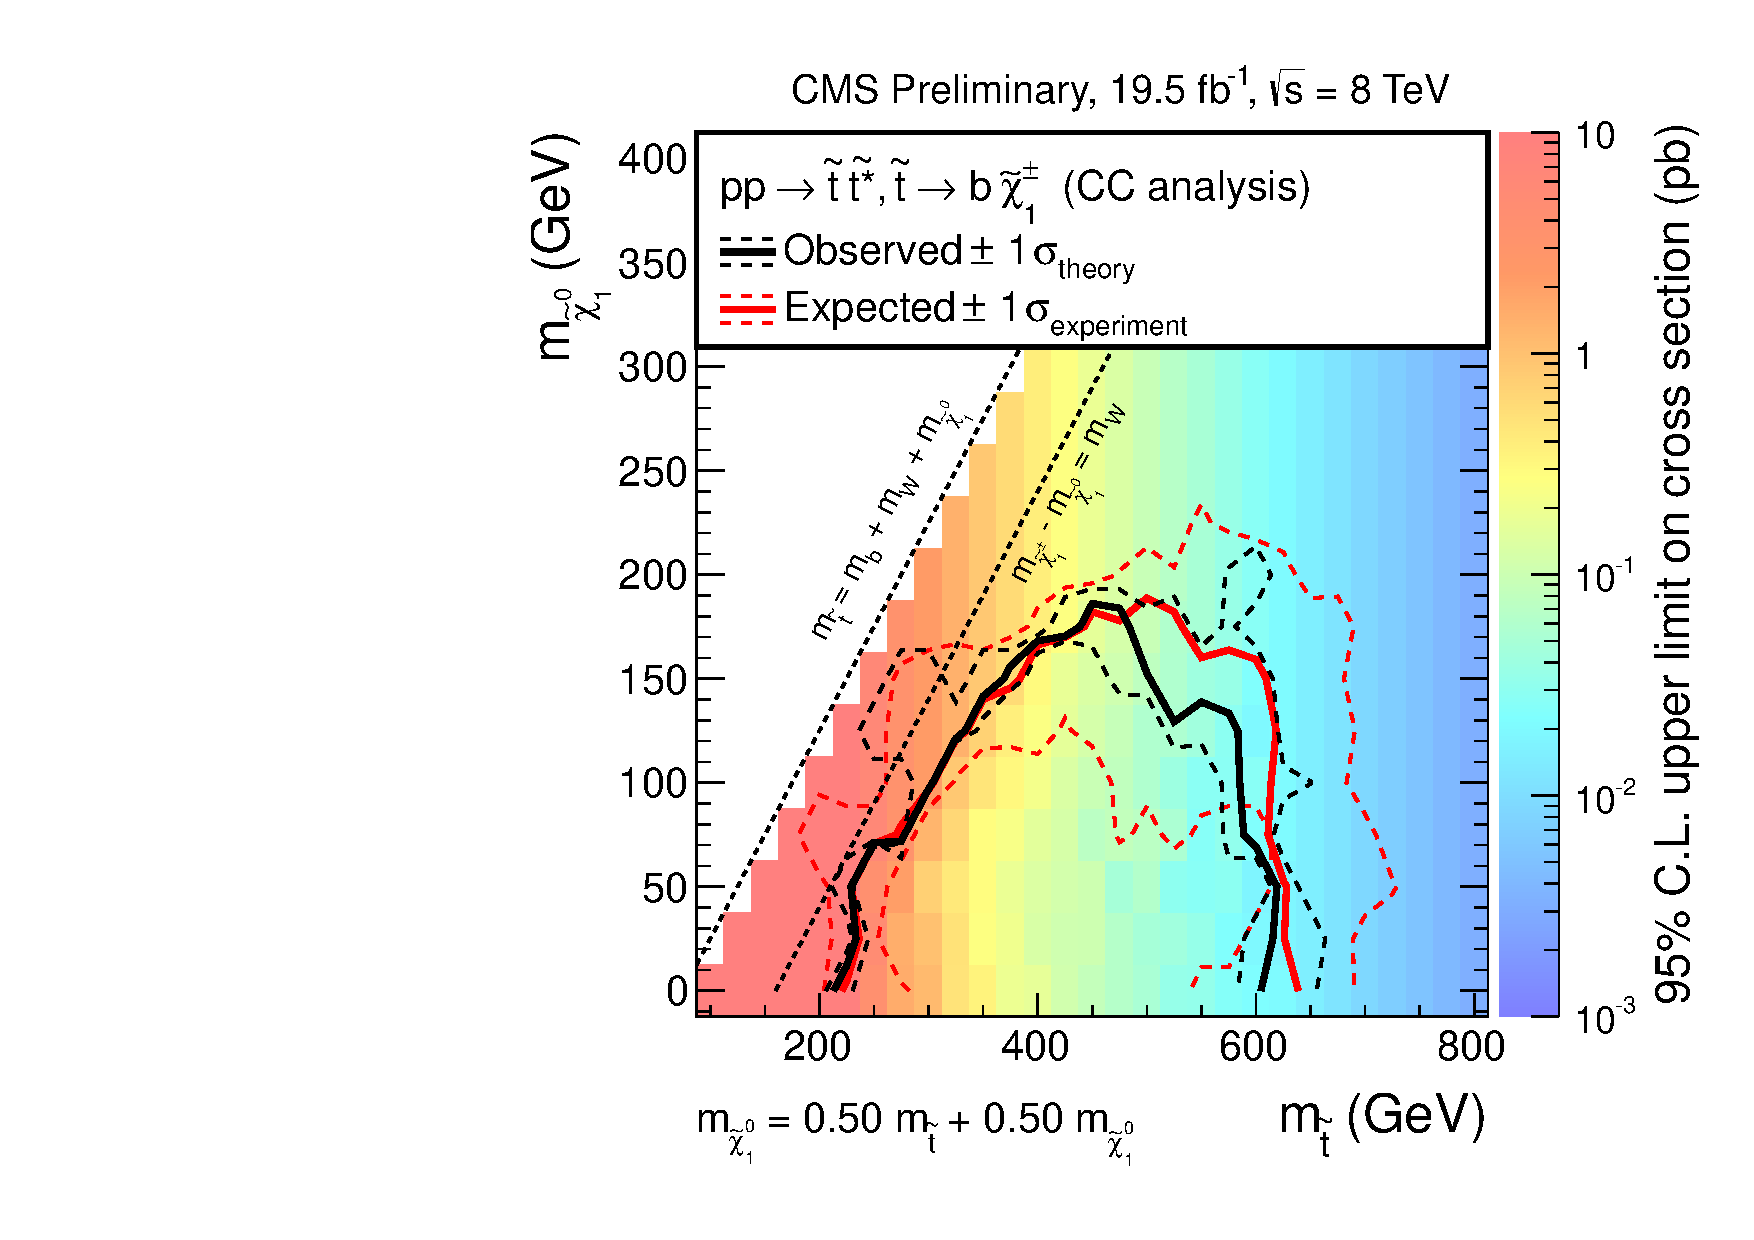
\includegraphics[width=0.31\textwidth]{limits/T2bw050_CC}\\
        \includegraphics[width=0.33\textwidth]{results/CnC_T2bw025/signalRegion_MTtail_yield}
        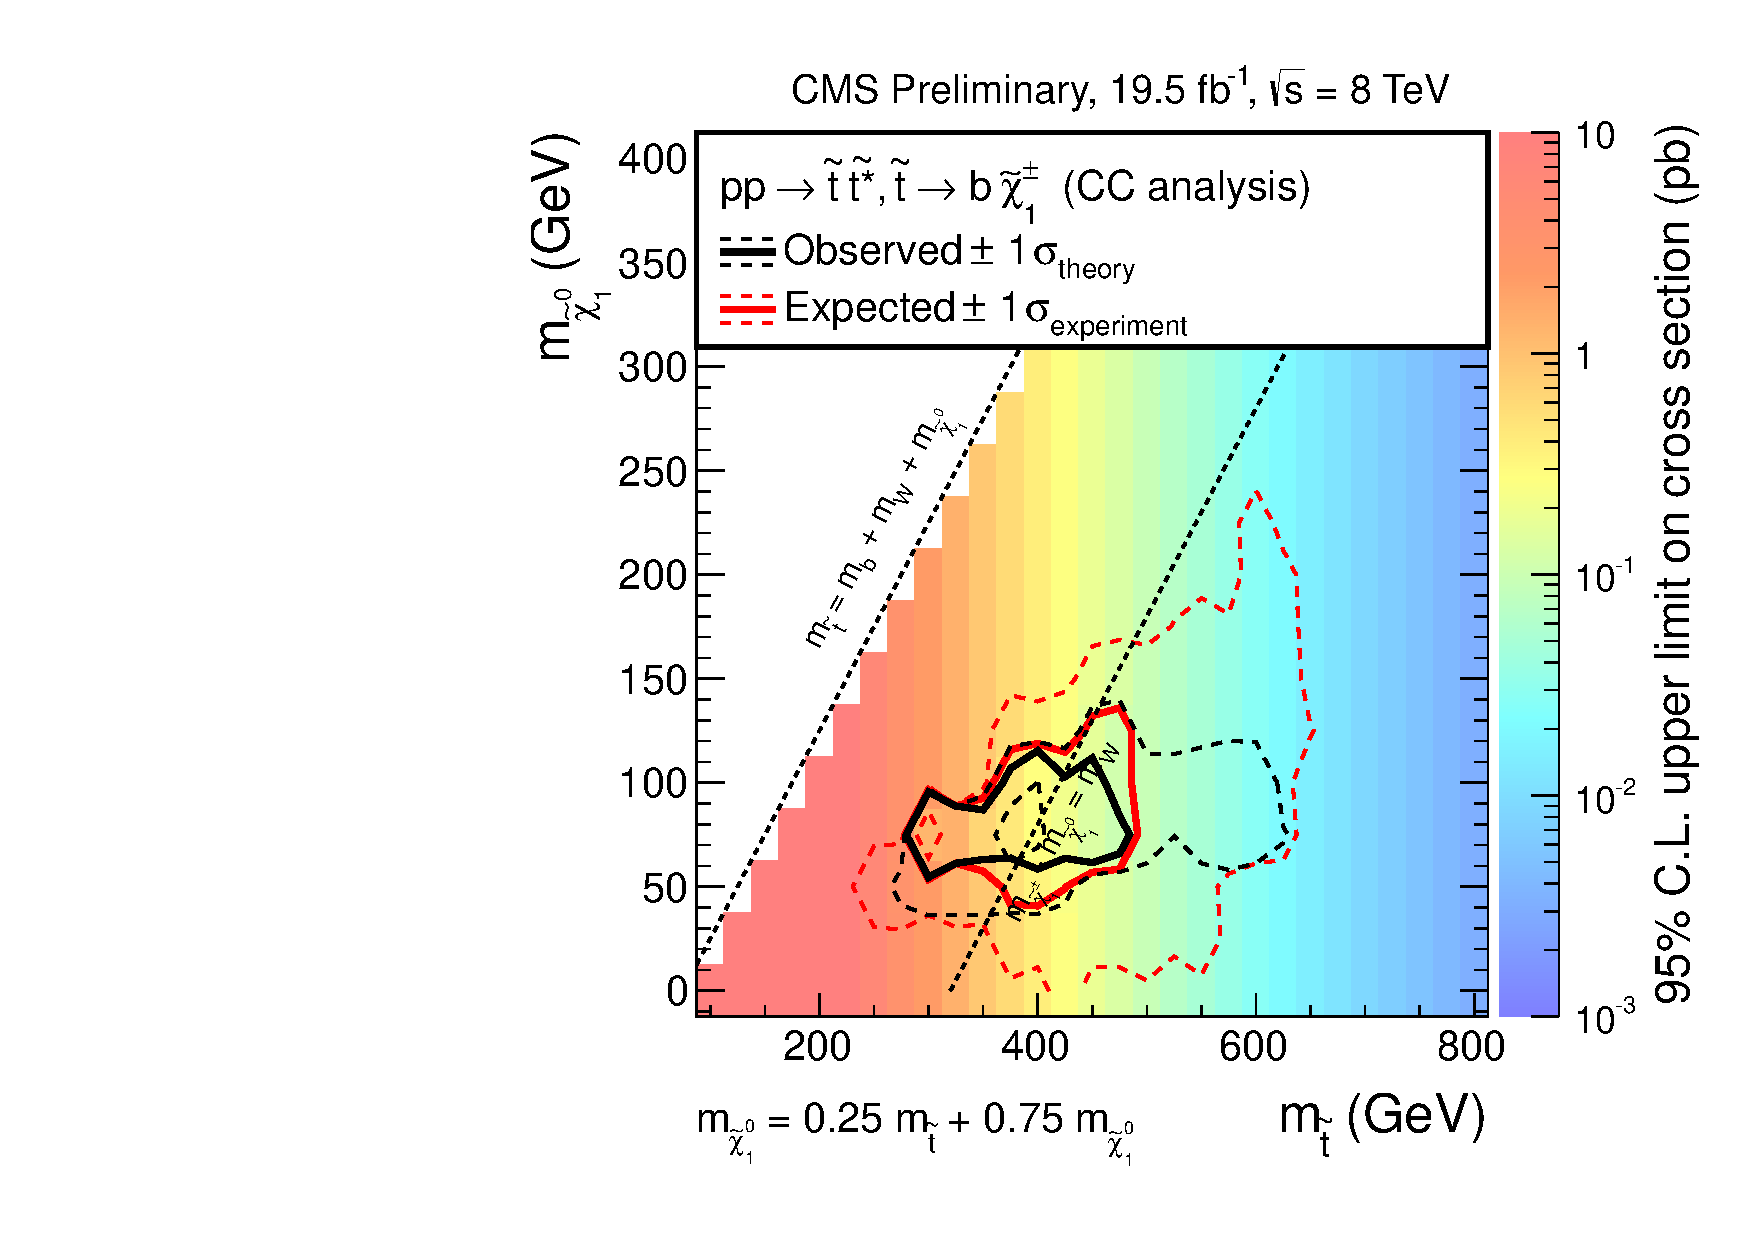
\includegraphics[width=0.31\textwidth]{limits/T2bw025_CC}\\
        \caption{On the left : comparison of the yield of the different cut-based signal
        regions between data and the background prediction under the null hypothesis. The
        grey hatching represents the systematic uncertainty, propagated on the ratio plot.
        On the right : upper limit at 95\% confidence level and exclusion in terms of
        $(\mass{\lstop},\mass{\lneutralino})$ after comparison to the theory, assuming
        $BR = 1$. On the first row, for $\lstop \rightarrow t \lneutralino$ decay mode on
        the second, third and last row for $\lstop \rightarrow b \lchargino$ decay mode
        with $x=0.75$, $0.50$ and $0.25$ respectively.}
        \label{fig:resultsCnC}
    \end{figure}

    \begin{figure}[h!]
        \centering
        \includegraphics[width=0.33\textwidth]{results/BDT_T2tt/signalRegion_MTtail_yield}
        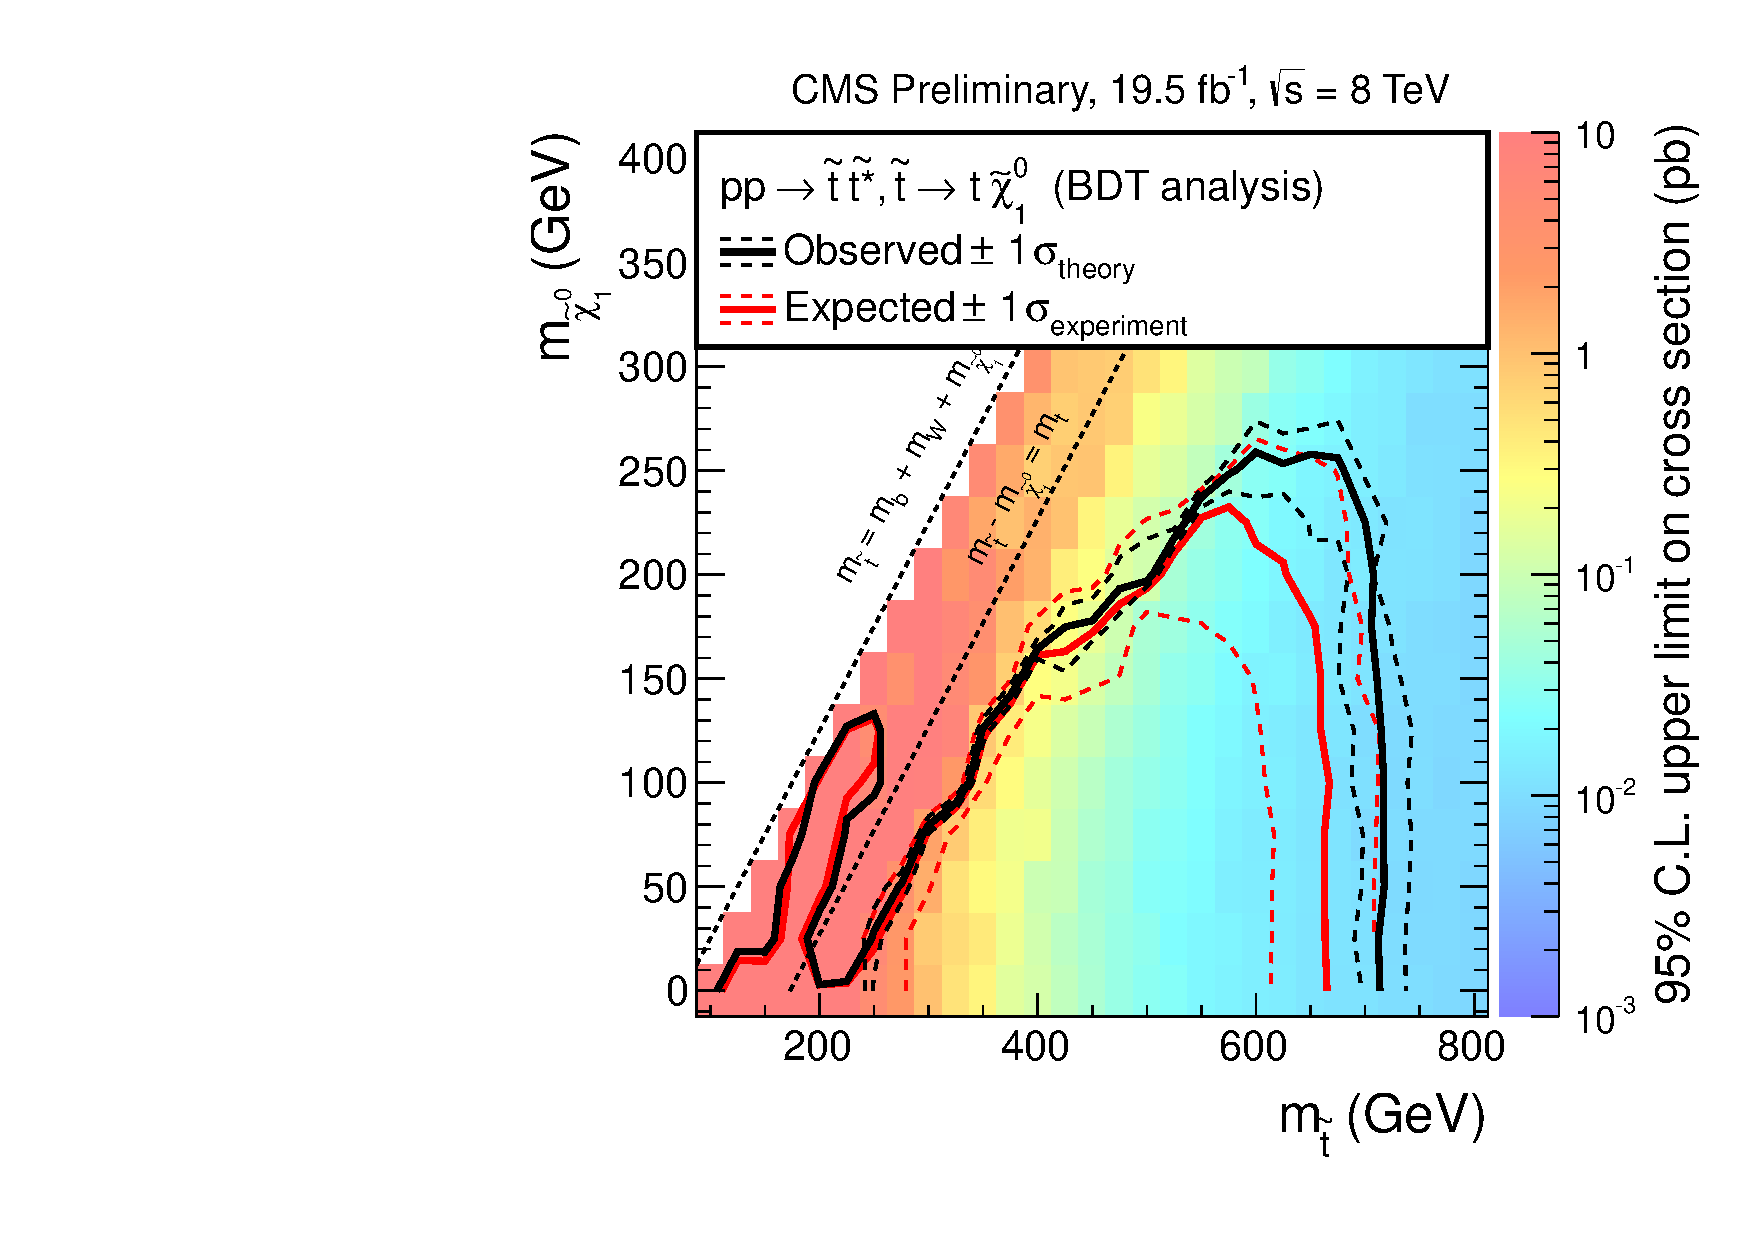
\includegraphics[width=0.31\textwidth]{limits/T2tt_BDT}\\
        \includegraphics[width=0.33\textwidth]{results/BDT_T2bw075/signalRegion_MTtail_yield}
        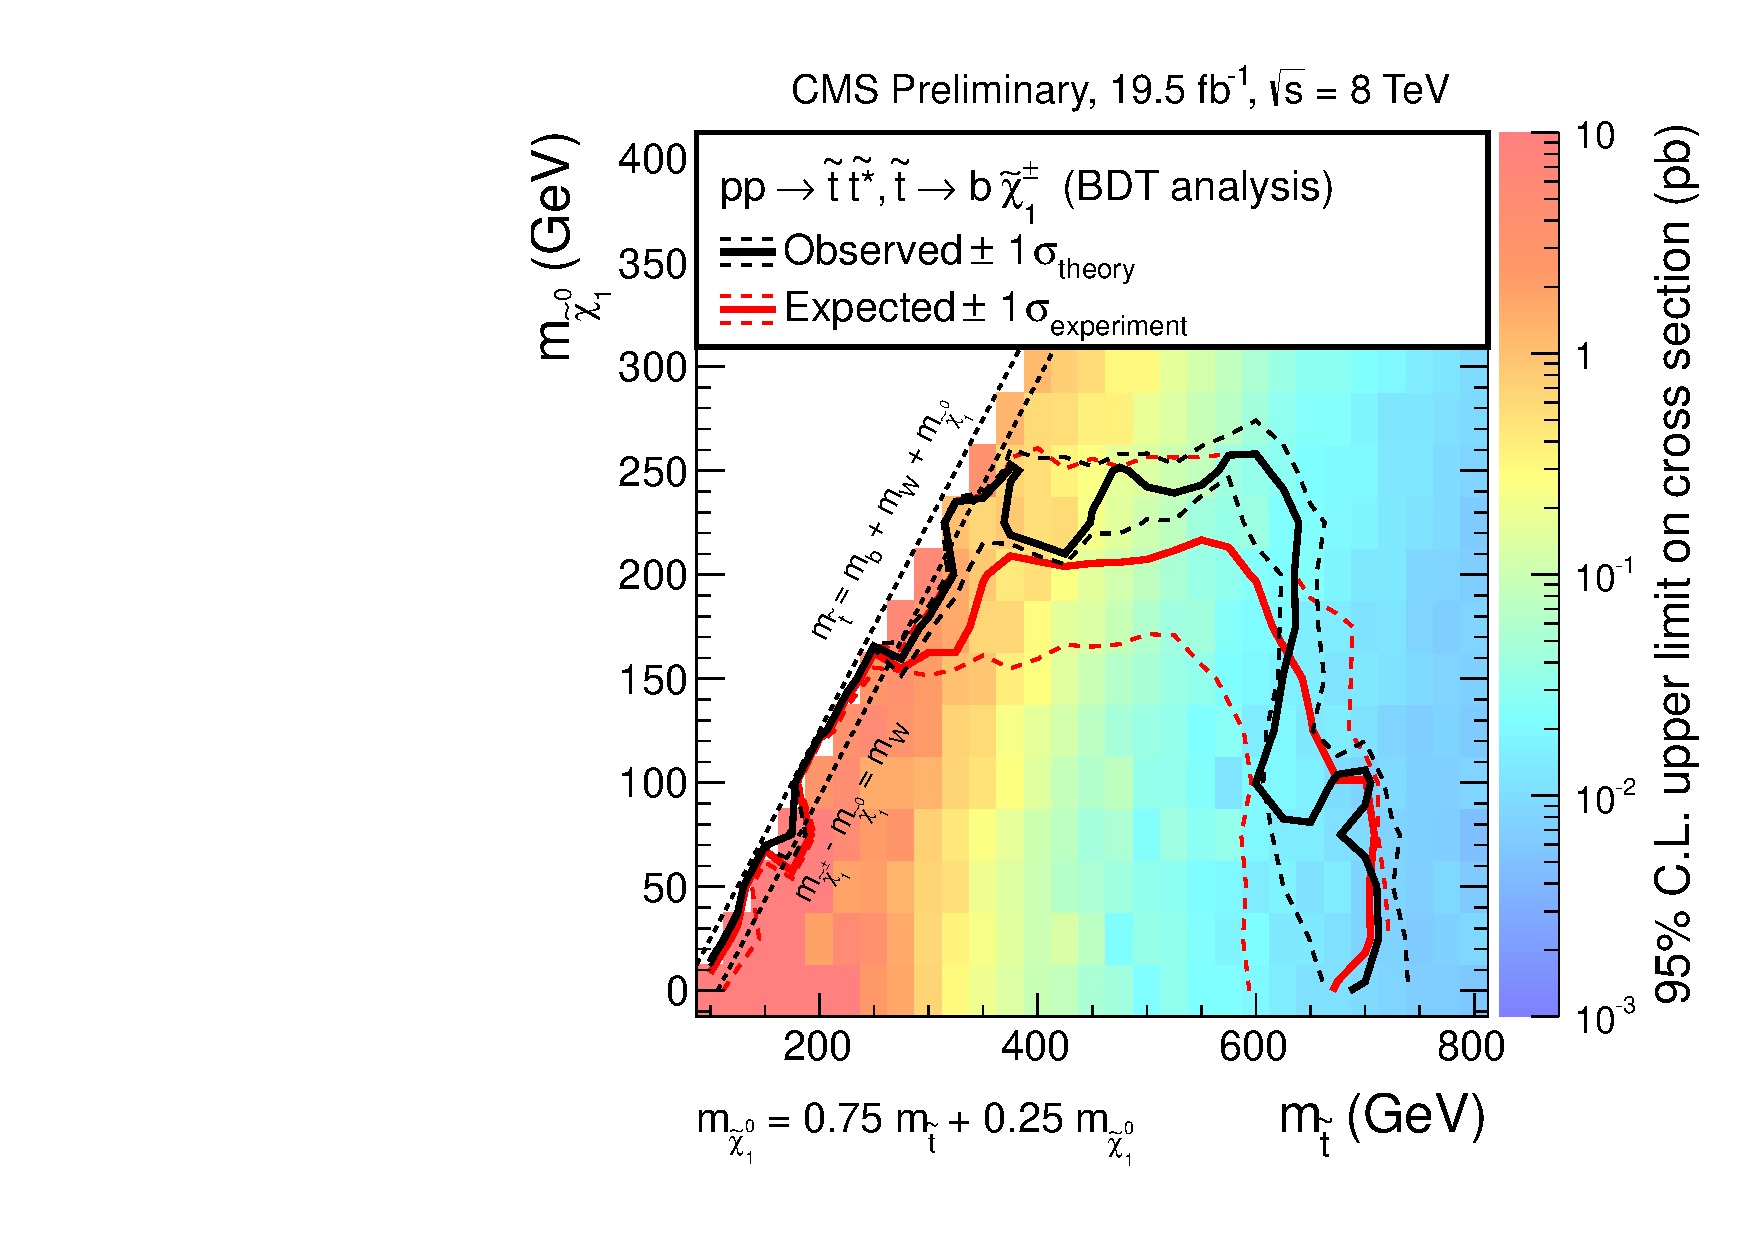
\includegraphics[width=0.31\textwidth]{limits/T2bw075_BDT}\\
        \includegraphics[width=0.33\textwidth]{results/BDT_T2bw050/signalRegion_MTtail_yield}
        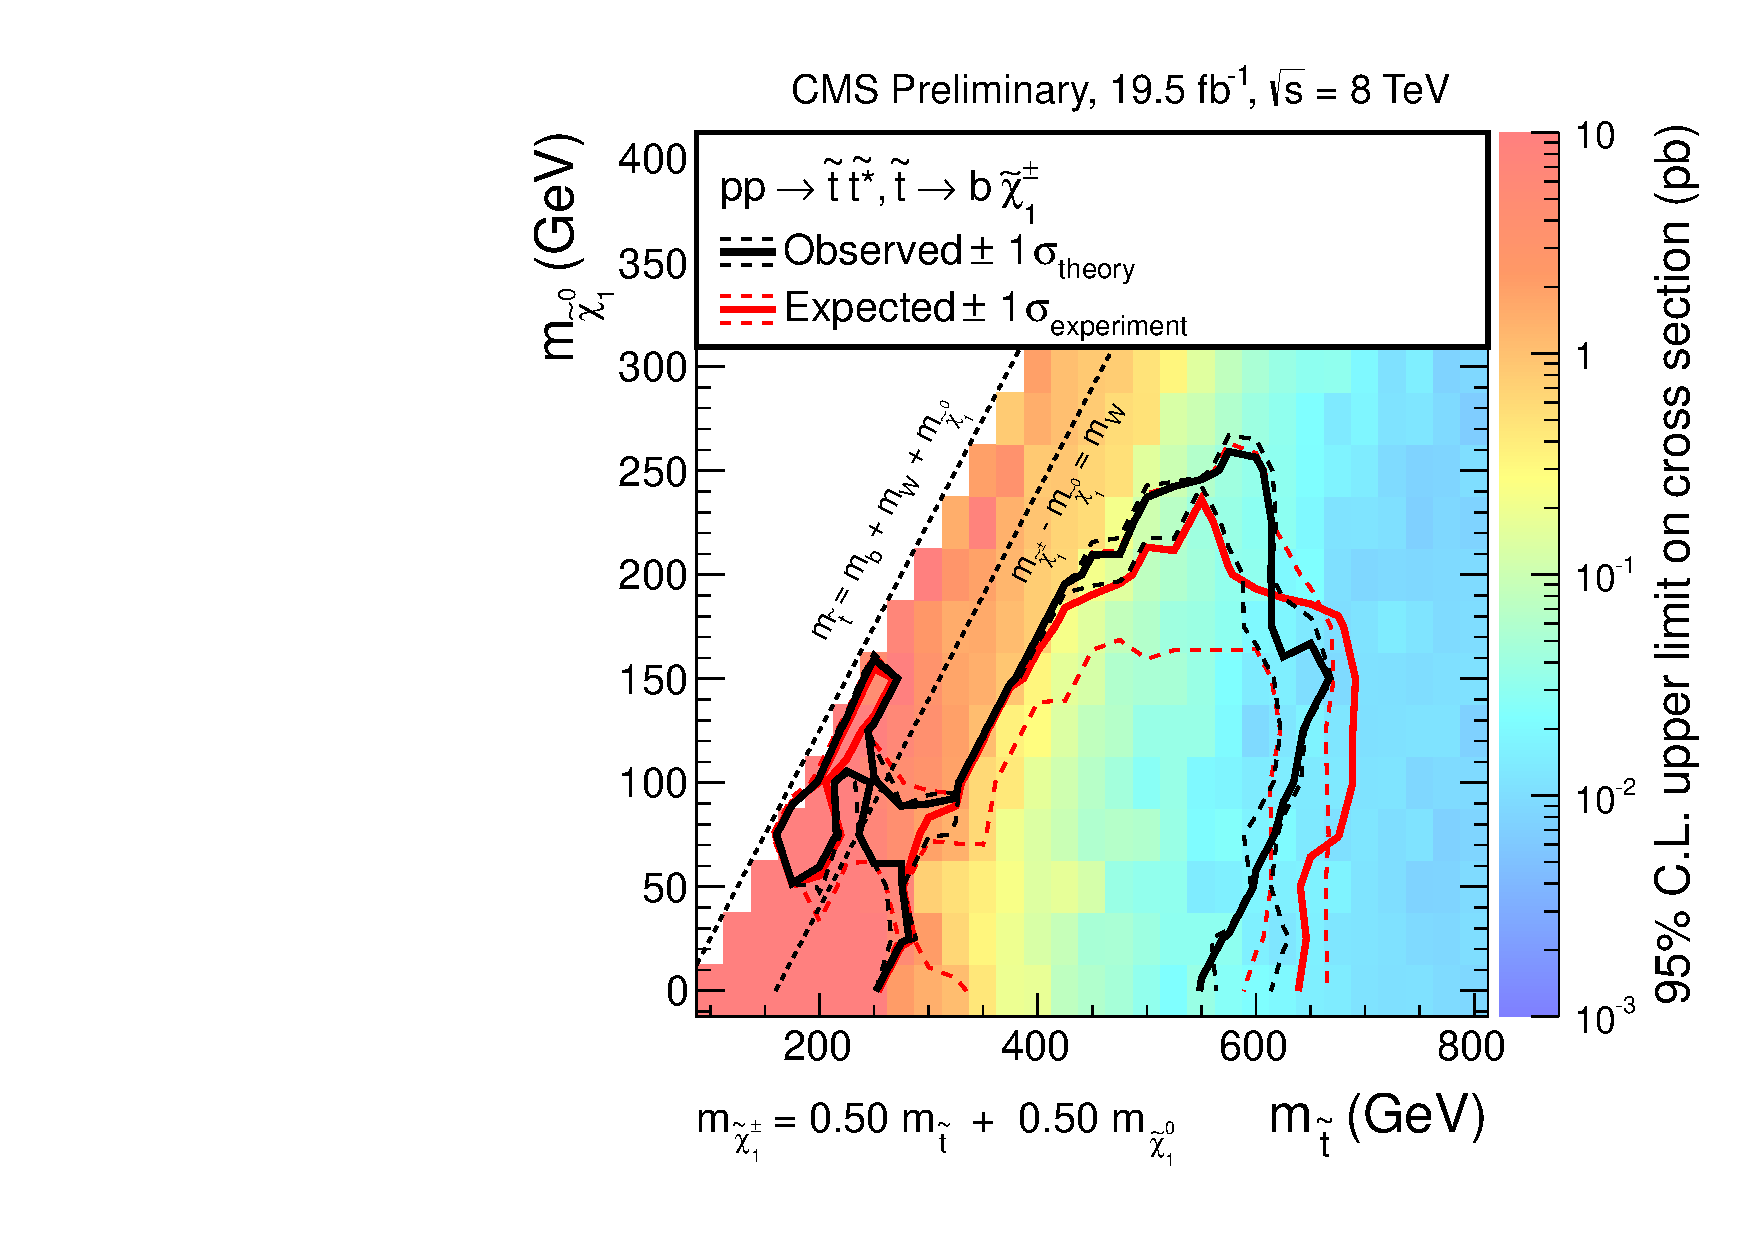
\includegraphics[width=0.31\textwidth]{limits/T2bw050_BDT}\\
        \includegraphics[width=0.33\textwidth]{results/BDT_T2bw025/signalRegion_MTtail_yield}
        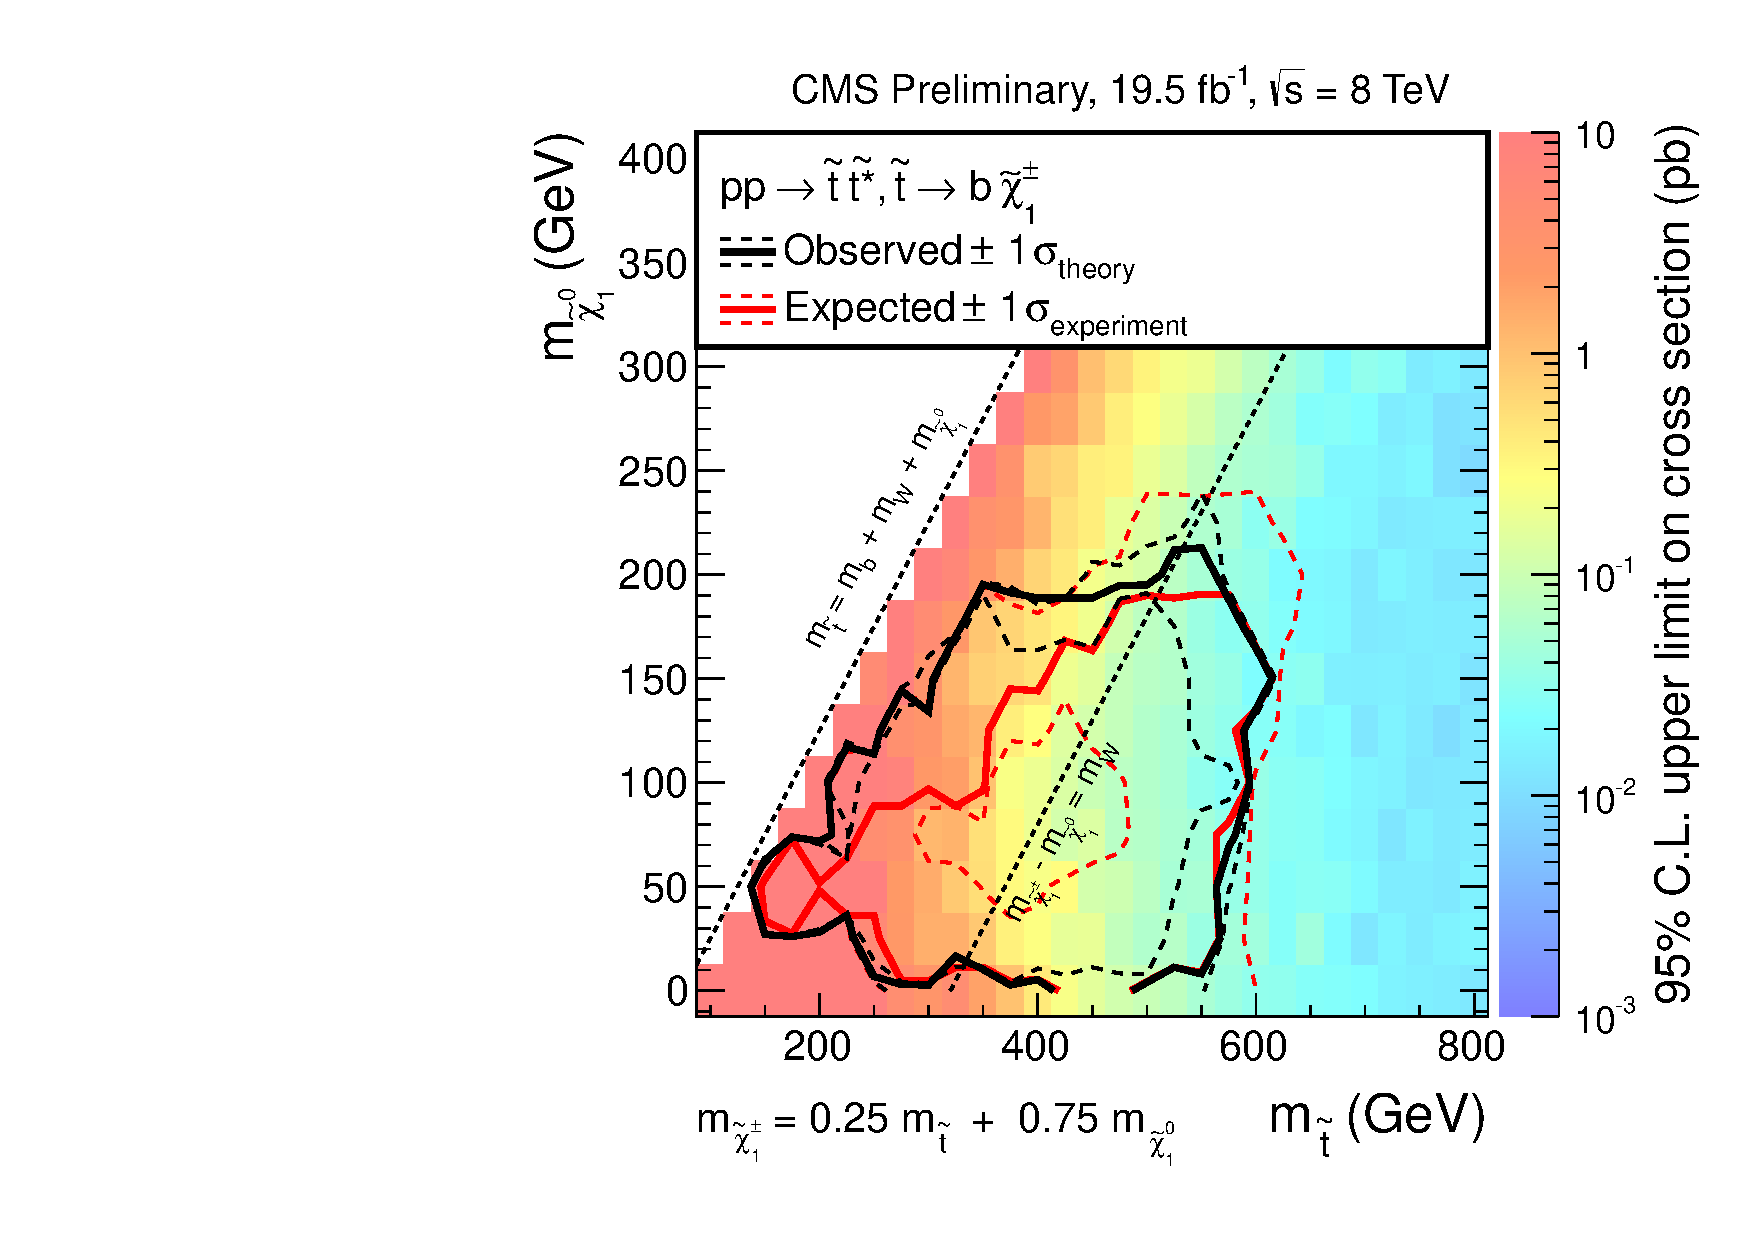
\includegraphics[width=0.31\textwidth]{limits/T2bw025_BDT}\\
        \caption{On the left : comparison of the yield of the different BDT-based signal
        regions between data and the background prediction under the null hypothesis. The
        grey hatching represents the systematic uncertainty, propagated on the ratio plot.
        On the right : upper limit at 95\% confidence level and exclusion in terms of
        $(\mass{\lstop},\mass{\lneutralino})$ after comparison to the theory, assuming
        $BR = 1$. On the first row, for $\lstop \rightarrow t \lneutralino$ decay mode on
        the second, third and last row for $\lstop \rightarrow b \lchargino$ decay mode
        with $x=0.75$, $0.50$ and $0.25$ respectively.}
        \label{fig:resultsBDT}
    \end{figure}

    The BDT approach leads to limits which are usually about $50 \GeV$ futher compared to
    the cut-based approach. For the $\lstop \rightarrow t \lneutralino$ decay mode, the
    observed exclusion using the BDT approach goes up to $\mass{\lstop} \sim 700 \GeV$
    and $\mass{\lneutralino} \sim 250 \GeV$ in the on-shell region and up to
    $\mass{\lneutralino} \sim 125 \GeV$ in the off-shell region. It is however difficult
    to exclude the region $\deltam \sim \mass{t}$ as the kinematic here is very close to
    standard model $t\bar{t}$.

    \todo{To be added when available (for the CnC especially) : polarized limits, branching
    ratio variation, maybe replace BDT results by a comparison BDT <-> CnC. \\Combination
    with 2$\ell$}

    Alternative exclusion in terms of $(\mass{\lstop}, \mass{\lneutralino})$ are proposed
    for different branching ratio assumptions, as represented on Figure \ref{fig}.
    Different polarization assumptions are also being looked at on \ref{fig:} for both
    decay types and can have a significant impact

    Figure \ref{fig:event62838873} shows one of the most signal-like event in the
    high-$\deltam$ signal region of the cut-based approach for $\lstop \rightarrow t \lneutralino$.

    \insertFigure{event62838873}{0.9}
    {One of the most signal-like event for the $\lstop \lstop^{*} \rightarrow t t \lneutralino \lneutralino$ decay-mode in the high-$\deltam$ cut-based approach. The event has one muon with $\pT = 114\GeV$, 4 jets among which 2 $b$-tag, $\MET = 392\GeV$ and $\MT = 300 \GeV$. Only tracks coming from the primary vertex are shown.}

    \newpage

    \section{Perspectives \label{sec:analysis_perspective}}
    %==============================================================

    \subsection{$W$-tagging in the high $\Delta m$ regime}

            \subsubsection{Motivation}

             As one considers higher $\Delta m$ values for the signal, the mean momentum of
             decay products increases. In particular, if we consider the hadronically
             decaying $W$, an increase of the $\pT$ translates into more colimated objects,
             in that case the pair of quarks that will hadronize. This is illustrated on
             the Figure \ref{fig:wTagging/ptW_vs_genDeltaRqq_fromttbar} showing the
             distribution of the $\Delta R$ between the
             quarks coming from the decay of a $W$ boson against the $\pT$ of the generated
             $W$. In the situation were the $\Delta R$ between the quarks approaches the
             size parameter used by the standard clustering algorithm (i.e. $\Delta R
             \sim 0.5$), only one big jet gets reconstructed instead of two smaller ones.
             This topology is refered to as boosted hadronic $W$.

             \insertFigure{wTagging/ptW_vs_genDeltaRqq_fromttbar}{0.5}{Distribution of
             the $\Delta R$ between the quarks coming from the decay of an hadronic $W$,
             as function of the generated $\pT$ of the $W$. The mean $\Delta R$ approaches
             0.5, the standard size parameter used at 8 TeV, at $\pT \sim 200\GeV$,
             meaning that jets coming from the quark will be merged by the clustering
             algorithm.}

             Driven by the fact that some new physics signatures are expected to contain
             such boosted hadronic $W$ \refNeeded, techniques have been developped to
             address this topology by providing variables to tag jets originating from
             boosted $W$ decays. The strategy consists in using a wider radius parameter
             when clustering the jets, clean and correct the jets from pile-up contamination,
             and analyze the substructure of the jets to derive variables that discriminate
             between boosted $W$ decays and fakes.

             Figure \ref{fig:} illustrate the interest that these technique might have to
             select the signal : the mean $\pT$ of the generated
             $W$ bosons for the signal accross the $(\mass{\lstop}, \mass{\lneutralino})$
             space grows as function of $\deltam$. For $\deltam > 650\GeV$, the
             mean $\pT$ is about $200\GeV$ and we can expect a large fraction of boosted $W$.
             Figure \ref{fig:} compares the distribution of the $\pT$ of the hadronic $W$ for one
             particular signal benchmark at high-$\deltam$ against the different backgrounds
             and shows that the presence a boosted $W$ tends to be discriminating.

             \insertTwoFigures{genWPtForSignal}
                              {wTagging/T2tt_meanGenWPt}{wTagging/genWPt_backgroundVsSignal}{0.4}
                              {On the left : mean $\pT$ of the generated $W$ for the
                              signal across the $(\mass{\lstop}, \mass{\lneutralino})$ space.
                              On the right : comparison of the $\pT$ spectra of the generated
                              hadronic $W$ for the $\oneLeptonTop$ and rare backgrounds and
                              the signal benchmark $(\mass{\lstop}, \mass{\lneutralino}) = (700,25) \GeV$.
                              The $\diLeptonTop$ and $\Wjets$ background are not represented
                              as they do not contain a generated hadronic $W$ by definition.}

            \subsubsection{Selection and performances}

            As an alternative to the standard anti-$k_T$ clustering algorithm with a
            size parameter $R = 0.5$ (AK5), an other jet collection is built using the
            Cambridge-Aachen clustering algorithm with a size parameter $R = 0.8$ (CA8).
            \todo{Add a reference to the detector chapter where AK, CA and kt are
            presented/compared ?}\todo{Comparison between CA and AK performances for jet
            substructure done in http://arxiv.org/pdf/0903.5081v4.pdf justifies the
            choice of CA8}

            To clean the jet from pile-up contributions and improve rejection of
            quark/gluon jets, a grooming technique called pruning is applied. It
            consists in reclustering the jet and applying
            conditions on the protojets during the algorithm, that vetos combinations of
            soft protojets with harder ones, or large angular combinations.
            \todo{Ref needed : JME-13-006, arXiv:0903.5081v4, + add sketch of grooming techniques}

            The substructure of the jet is analyzed via the $N$-subjetiness variables,
            which are designed to quantify how likely a jet is to be composed of $N$
            sub-jets. \todo{Ref to arXiv:1011.2268v3} These variables are denoted $\tau_1$,
            $\tau_2$, ... $\tau_N$. A value close to 0 for $\tau_N$ tends to indicate
            a good compatibility with the $N$-subjets hypothesis. In the context of
            $W$-tagging, it is common to focus on the use of the ratio $\tau_2/\tau_1$
            which provides good discrinability between real $W$ and quark/gluons jets.

            To define selection criteria, we study the distribution of a few variables
            on a $t\bar{t}$ Monte-Carlo sample after applying the preselection defined in
            \ref{sec:analysis_objectAndEventSelection}. We however allow events with at
            least 3 jets instead of 4. $W$ candidates are matched to generated
            hadronically-decaying $W$ : if the candidate is within $\Delta R < 0.4$, it
            is considered as matched, whereas candidates which are in $\Delta R > 2$ are
            considered to be fakes originating from quark or gluons. We studied the
            prunned mass of the jet, the $N$-subjetiness ratio $\tau_2 / \tau_1$ and the
            distance to the selected lepton $\Delta R (\ell,\text{jet})$.

            Figure \ref{fig:wTaggingVariables} shows the distribution of the prunned mass of
            the jet and the $N$-subjetiness ratio $\tau_2 / \tau_1$ for candidates with
            $\pT > 150\GeV$ and with $\Delta R(\ell,\text{jet}) > 1.5$. A good working point
            is found to be $\text{mass}(\text{jet} > 70\GeV)$ and $\tau_2 / \tau_1 < 0.5$.
            The resulting tagging efficiency is estimated as function of the $\pT$ of the
            candidate as presented on \ref{fig:wTagging/taggingEfficiency_fromttbar}.
            The efficiency for candidates matched
            to true $W$ is about 30\% at $200\GeV$ and plateau to 70\% at $270\GeV$. It
            however starts decreasing around $350\GeV$ as it gets more difficult to resolve
            the two subjets. The fake rate is about 5\% for candidates of $200\GeV$ and
            grows linearly with the $\pT$ as momentum tends to create unphysical large
            mass for the jets.

            \insertTwoFigures{wTaggingVariables}
                             {wTagging/prunnedMassAfterBasicSelection_fromttbar}
                             {wTagging/tau2OverTau1AfterBasicSelection_fromttbar}
                             {0.4}
                             {Distribution of the prunned mass (on the left) and $\tau_2
                             / \tau_1$ for CA8 jets with $\pT > 150\GeV$ and
                             $\Delta R(\ell,\text{jet}) > 1.5$ in $t\bar{t}$ events
                             with preselection applied.}

            \insertFigure{wTagging/taggingEfficiency_fromttbar}{0.5}
                         {Tagging efficiency for the true $W$ jets and fakes from quark/gluon
                         jets, as function of the $p_T$ of the jet.}

            \subsubsection{Impact on the analysis sensitivity}

            \todo{... Take one high deltamM benchmark for example, split in two channels
            0Wtag, 1Wtag. Apply standard/current selection on 0Wtag. Tune cuts for
            1Wtag. Measure sensitivity of each box+combine(need to fin how). Compare to
            current analysis with no Wtag at all. Conclude wether or not it is providing
            an increase of sensitivity. Plot as function of mStop at constant mNeutralino.}

        \subsection{Sensitivity and perspectives for the Run II}
        % =====================================================

        \loremipsum

            \subsubsection{Extrapolation of the sensitivity from Run I analysis}
        % =====================================================

        One can get a basic estimation of the integrated luminosity $\mathcal{L}$ required
        at 13 TeV to obtain equivalent sensitivity compared to 8 TeV, starting from the
        following equation :

        $$ \left( \frac{S}{\sqrt{B}} \right)_{8\TeV} = \left( \frac{S}{\sqrt{B}} \right)_{13\TeV}  $$

        Using $N = \mathcal{L} \times \sigma \times \epsilon$ and assuming that the selection
        efficiencies $\epsilon$ remain the same between $8$ and $13\TeV$, one finds that

        $$ \mathcal{L}^\text{equiv.}_{13\TeV} = \mathcal{L}_{8\TeV} \times \frac{\kappa_B}{\kappa^2_S} $$

        where $\kappa \definedAs \sigma_{13\TeV} / \sigma_{8\TeV}$. For $\mass{\lstop} \sim 800\GeV$,
        $\kappa_S \sim 10$. From the experience at $8\TeV$ using the high-$\deltam$ selection,
        the dominant backgrounds are $t\bar{t}$ and $t\bar{t}+Z$. For these processes, one
        gets $\kappa_B \sim 3.3$. One ends up with

        $$ \mathcal{L}^\text{equiv.}_{13\TeV} \sim 0.7\invfb$$

        The sensitivity has been further studied on two Monte-Carlo benchmarks for the
        $\lstop \rightarrow t \lneutralino$ signal type with $(\mass{\lstop},
        \mass{\lneutralino}) = (650,325)$ and $(850,100) \GeV$. An object selection
        strongly inspired from \ref{sec:analysis_objectAndEventSelection}, though simplified
        for this study, was used. A similar preselection is applied, requiring one electron
        or muon with $p_T > 30\GeV$, at least four jets among which one $b$-tagged, at least
        50 \GeV for $\MET$ and vetoing on a second lepton with $p_T > 5\GeV$. Table \ref{tab:phys14Preselection}
        shows the Monte-Carlo yields for $\mathcal{L} = 1\invfb$ obtained at preselection
        and after cutting on $\MT > 120\GeV$.

        \begin{table}
            \centering
                \begin{tabular}{|l|cc|}
        \hline
        &
        \textbf{preselection}   &
        \textbf{ + $M_{T}$ > 120 GeV}                                 \\
        \hline
        \textbf{$\oneLeptonTop$} & 9868  $\pm$ 18    & 614 $\pm$ 4     \\
        \textbf{$\diLeptonTop$}  & 2073  $\pm$ 8     & 1039 $\pm$ 5    \\
        \textbf{$W$+jets}        & 908   $\pm$ 74    & 55 $\pm$ 18     \\
        \textbf{rare}            & 148   $\pm$ 10    & 36 $\pm$ 3      \\
        \hline
        \textbf{total SM}        & 12998 $\pm$ 77    & 1745 $\pm$ 20   \\
        \hline
        \textbf{\textsc{T2tt} (850/100)}  & 2.57  $\pm$ 0.02  & 2.18 $\pm$ 0.02 \\
        \textbf{\textsc{T2tt} (650/325)}  & 12.11 $\pm$ 0.11  & 8.89 $\pm$ 0.09 \\
        \hline
    \end{tabular}

            \caption{\todo{To be updated with higher stat} \label{tab:phys14Preselection}}
        \end{table}

        We define three signal regions SR 1, 2 and 3 inspired from the high-$\deltam$
        selection at $8\TeV$ using only increasing cuts on $\MET$ and $\MTTwoW$ as defined
        on Table \ref{tab:phys14Cuts}. Table \ref{tab:phys14SignalREgions} shows the yield
        obtained from Monte-Carlo assuming $\mathcal{L} = 1\invfb$.

        \begin{table}
            \centering
            \begin{tabular}{c|cc}
                \textbf{Signal Region} & $E_T^\text{miss}$ & $M_{T2}^W$ \\
                \hline
                \textbf{SR1}           & >250 & >180 \\
                \textbf{SR2}           & >300 & >190 \\
                \textbf{SR3}           & >350 & >200 \\
            \end{tabular}
            \caption{\todo{Write caption} \label{tab:phys14Cuts}}
        \end{table}

        \begin{table}
            \centering
            \begin{tabular}{|l|ccc|}
\hline
&
\textbf{SR1}     &
\textbf{SR2}     &
\textbf{SR3}     \\
\hline
\textbf{$t\bar{t}$}      & 16.33 $\pm$ 7.30    & 0.00 $\pm$ 0.00    & 0.00 $\pm$ 0.00      \\
\textbf{$W$+jets}        & 0.00 $\pm$ 0.00     & 0.00 $\pm$ 0.00    & 0.00 $\pm$ 0.00      \\
\textbf{$t\bar{t}V$}     & 1.81 $\pm$ 0.09     & 1.06 $\pm$ 0.07    & 0.63 $\pm$ 0.06      \\
\hline
\textbf{total SM}        & 18.13 $\pm$ 7.30    & 1.06 $\pm$ 0.07    & 0.63 $\pm$ 0.06      \\
\hline 
\textbf{T2tt (850/100)}  & 1.41 $\pm$ 0.02     & 1.25 $\pm$ 0.02    & 1.08 $\pm$ 0.01      \\
\textbf{T2tt (650/325)}  & 2.90 $\pm$ 0.05     & 2.01 $\pm$ 0.05    & 1.27 $\pm$ 0.04      \\
\hline
\end{tabular}

            \caption{\todo{To be updated with higher stat} \label{tab:phys14SignalRegions}}
        \end{table}

       Finally, the sensitivity is estimated from the results in the SR2 region, as function
       of the integrated luminosity using $S / \sqrt{B + f^2 B^2}$ with a relative systematic
       uncertainty of $f = 50\%$ on the background. The results are presented on Figure
       \ref{fig:} and suggest that a signal with $(\mass{\lstop}, \mass{\lneutralino}) = (850,100)$
       could be excluded with $\mathcal{L} = 4\sim5\invfb$ or put in evidence with
       $\mathcal{L} = 10\sim15\invfb$.

            \insertFigure{phys14/sensitivityAsFunctionOfLumi}
                         {0.9}
                         {\todo{To be updated with higher stat (and maybe put discoverable/excluded signal strength instead ?)}}

         \subsection{Expected benefits from new object reconstruction and selection techniques}
         % =====================================================

            Techniques :
            \begin{itemize}
                \item PUPPI jets, PUPPI MET ?
                \item new isolation, ..?
                \item statistical interpretation using multiple bin to simultaneously fit S and B ? (ie simplify signal contamination treatment)
            \end{itemize}

            Variables :
            \begin{itemize}
                \item MT deconstruction, allowing to have more control to the regime looking at ? e.g. lower lepton pT  at low deltaM, more reliance on deltaPhi ?
                \item ISR tagging improvement
                \item Topness ?
                \item reduce lepton threshold ? how to probe high neutralino regime, low deltaM ?
                \item Build a 'MT significance' ?
            \end{itemize}

    \section{Overview of related searches for top partner in CMS \label{sec:analysis_overviewStopSearches}}
    %==============================================================

        \begin{itemize}
            \item Direct stop 0l (SUS-13-023)
            \item Direct stop 2l (?)
            \item Compressed spectra, monojet (SUS-13-009)

                % SUS-13-009, based on ISR, main background is Z->vv+jets and W+jets, most sensitive in low deltaM region (monojet-like events)
% the first problem is with triggering these events : the jets and leptons originating from the stop decays are too soft to be used during the online selection. The only possibility is to consider these processes with ISR with a consequent reduction in the effective cross section.

            \item Compressed spectra, soft leptons (SUS-14-021)
            \item Razor searches, gluino-mediated production ?
            \item Combinaison SUS-13-011 + Razor 0l ?? (SUS-13-011)
            \item Search for t2 -> H t1 -> ... ?
            \item Indirect searches for stealth region, using cross section measurement / spin correlation
        \end{itemize}


%==============================================================
\chapter{???}
%==============================================================
        \loremipsum


%==============================================================
\chapternonum{Conclusion}
%==============================================================
        \loremipsum





\begin{thebibliography}{2}

\addcontentsline{toc}{chapter}{Bibliography}

\singlespace

\addReference{EllisDarkMatter}
             {J. Ellis, K. A. Olive}
             {Supersymmetric Dark Matter Candidates}
             {arXiv:1001.3651}

%====================================
%Naturalness, stop motivation related
%====================================

\addReference{LEPparadox}
             {R. Barbieri, A. Strumia}
             {The `LEP paradox'}
             {arXiv:hep-ph/0007265v2}

\addReference{LectureStandardModelHiggsBoson}
             {I. van Vulpen, A. Castelli}
             {Lecture on Particle Physics II, 2011-2012, The Standard Model Higgs Boson}
             {http://master.particles.nl/LectureNotes/2011-PPII-Higgs.pdf}

%\addReference{Naturalness}
%             {S. Dimopoulos, G.F. Giudice}
%             {Naturalness Constraints in Supersymmetric Theories with Non-Universal Soft Terms.}
%             {arXiv:hep-ph/9507282}

%\addReference{}
%Baryogenesis (to read)
%http://www.slac.stanford.edu/econf/C0508141/proc/pres/ALCPG0333_TALK.PDF
%https://kicp-workshops.uchicago.edu/DM-LHC2013/depot/talk-carena-marcela.pdf
%arXiv: 1009.3969, arXiv:1110.4378,
%http://arxiv.org/pdf/1207.6330v2.pdf
%http://arxiv.org/pdf/hep-ph/0404184v1.pdf

%=================
%Simplified models
%=================

\addReference{LiemSMS}
             {S. Liem}
             {Constraining Supersymmetry using Simplified Models}
             {urn:nbn:se:su:diva-91365}

\addReference{SmodelS}
             {S. Kraml et al.}
             {SModelS: a tool for interpreting simplified-model results from the LHC and its application to supersymmetry}
             {arXiv:1312.4175v3}

%=======================
% Generator, setup
%=======================

\addReference{Powheg}
             {S. Frixione, P. Nason, C. Oleari}
             {Matching NLO QCD computations with Parton Shower simulations: the POWHEG method}
             {arXiv:0709.2092}

\addReference{Madgraph}
             {J. Alwall et al.}
             {MadGraph 5 : Going Beyond}
             {arXiv:1106.0522}

\addReference{Pythia}
             {T. Sjostrand, S. Mrenna, P. Skands}
             {Pythia 6.4 Physics and Manual}
             {arXiv:hep-ph/0603175}

%===================
% POG and PAG stuff
%===================

\addReference{METperf}
             {The CMS Collaboration}
             {Missing transverse energy performance of the CMS detector}
             {arXiv:1106.5048}

%=============
%Polarization
%=============

\addReference{polarization1}
             {M. Perelstein, A. Weiler}
             {Polarized Tops from Stop Decays at the LHC}
             {arXiv:0811.1024v2}

\addReference{polarization2}
             {Ian Low}
             {Polarized Charginos (and Tops) in Stop Decays}
             {arXiv:1304.0491v2}

%=======================
%FOM-related, statistics
%=======================

\addReference{Punzi}
             {G. Punzi}
             {Sensitivity of searches for new signals and its optimization}
             {arXiv:physics/0308063v2}

\addReference{TMVA}
             {A. Hoecker et al.}
             {TMVA - Toolkit for Multivariate Data Analysis}
             {arXiv:physics/0703039}

%========
%Analysis
%========

\addReference{SUS-12-023-PAS}
             {The CMS Collaboration}
             {Search for direct top squark pair production in events with a single isolated lepton, jets and missing transverse energy at sqrt(s) = 8 TeV}
             {CMS Physics Analysis Summary SUS-12-023}

\addReference{SUS-13-011-PUB}
             {The CMS Collaboration}
             {Search for top-squark pair production in the single-lepton final state in pp collisions at sqrt(s) = 8 TeV}
             {Eur. Phys. J. C 73 (2013) 2677. arXiv:1308.1586}

\addReference{SUS-14-015-PAS}
             {The CMS Collaboration}
             {Search for direct stop pair production in the single lepton channel at sqrt(s)=8 TeV}
             {CMS Physics Analysis Summary SUS-14-015}

%==========
%MET/sqrt(HT), MET significance
%==========

\addReference{METsignificanceMirman}
             {N. Mirman, Y. Wang, J. Alexander}
             {Missing transverse energy significance at CMS}
             {arXiv:1409.3028v1}

%========
%ISR-related
%========

\addReference{ISRtagging}
             {D. Krohn, L. Randall, L. Wang}
             {On the Feasibility and Utility of ISR Tagging}
             {arXiv:1101.0810}

\addReference{ISRGluinoTevatron}
             {J. Alwall et al.}
             {Searching for Directly Decaying Gluinos at the Tevatron}
             {arXiv:0803.0019}

\addReference{ISRmodelingDominick}
             {The CMS Collaboration}
             {Hadronic Recoil Studies of Heavy Boosted Systems}
             {CMS Analysis Note 2013/059}

%===========
%Misc / tmp
%===========

\addReference{ClosingStopGap}
             {Michal Czakon et al.}
             {Closing the stop gap}
             {arXiv:1407.1043}

\end{thebibliography}




